\documentclass[twoside]{article}

\usepackage{aistats2025}
% If your paper is accepted, change the options for the package
% aistats2025 as follows:
%
%\usepackage[accepted]{aistats2025}
%
% This option will print headings for the title of your paper and
% headings for the authors names, plus a copyright note at the end of
% the first column of the first page.

% If you set papersize explicitly, activate the following three lines:
%\special{papersize = 8.5in, 11in}
%\setlength{\pdfpageheight}{11in}
%\setlength{\pdfpagewidth}{8.5in}

% If you use natbib package, activate the following three lines:
\usepackage[round]{natbib}
\renewcommand{\bibname}{References}
\renewcommand{\bibsection}{\subsubsection*{\bibname}}

% If you use BibTeX in apalike style, activate the following line:
%\bibliographystyle{apalike}

% custom packages
\usepackage[utf8]{inputenc} % allow utf-8 input
\usepackage[T1]{fontenc}    % use 8-bit T1 fonts
\usepackage{hyperref}       % hyperlinks
\usepackage{url}            % simple URL typesetting
\usepackage{booktabs}       % professional-quality tables
\usepackage{nicefrac}       % compact symbols for 1/2, etc.
\usepackage{microtype}      % microtypography
\usepackage{graphicx}
\usepackage{pgffor}
\usepackage{doi}
\usepackage{xfrac}
\usepackage{xcolor}
\usepackage{amsfonts}
\usepackage{amsmath}
\usepackage{bm}
\usepackage{bbold}
\usepackage{bbm}
\usepackage{subcaption}
\usepackage{array}
\usepackage{algorithm}
\usepackage{algpseudocode}
\usepackage{tikz}
\usepackage{mwe}
% \usepackage{xr}
% \usepackage[nokeyprefix]{refstyle}
% \externaldocument{supplement}

\hypersetup{
    colorlinks=true,
    linkcolor=blue,
    filecolor=magenta,      
    urlcolor=blue,
    citecolor=blue,
    }
% \usepackage{multirow}

% custom commands
\newcommand{\mub}{\boldsymbol{\alpha}}
\newcommand{\thb}{\boldsymbol{\theta}}
\newcommand{\ub}{\mathbf{u}}
\newcommand{\yb}{\mathbf{y}}
\newcommand{\vb}{\mathbf{v}}
\newcommand{\jac}{\mathbf{J}}
\newcommand{\data}{\mathbf{y}^o}
\newcommand{\accregioni}{C_{\epsilon}^i}
\newcommand{\danger}{\fontencoding{U}\fontfamily{futs}\selectfont\char 66\relax}
\newcommand{\TODO}[1]{\textcolor{red}{(to-do): #1}\marginpar{\textcolor{red}{\Large \danger}}}
\newcommand{\E}{\mathbb{E}}
\newcommand{\code}[1]{\mathtt{#1}}
\newcommand{\rromc}{R2OMC}
\newcommand{\corerromc}{\texttt{CoreR2OMC}}
\newcommand{\romc}{ROMC}
\newcommand{\nromc}{NAIVE-ROMC}
\newcommand{\REJ}{REJ-ABC}
\newcommand{\SMC}{SMC-ABC}
\newcommand{\NPE}{NPE}
\newcommand{\NLE}{NLE}
\newcommand{\NRE}{NRE}
\newcommand{\SNPE}{SNPE}
\newcommand{\SNLE}{SNLE}
\newcommand{\SNRE}{SNRE}
\newcommand{\CtwoST}{\texttt{C2ST}}
\newcommand{\Dparam}{D} % dimension of the parameter space
\newcommand{\mask}{\mathbf{m}_\tau}
\newcommand{\LinkToCode}{\textit{anonymized link}}
\newcommand{\approptoinn}[2]{\mathrel{\vcenter{
  \offinterlineskip\halign{\hfil$##$\cr
    #1\propto\cr\noalign{\kern2pt}#1\sim\cr\noalign{\kern-2pt}}}}}

\newcommand{\appropto}{\mathpalette\approptoinn\relax}

% for use in image printing
\newcommand{\imagerow}[3]{% #1 = prefix, #2 = label
  \raisebox{-.5\height}{\includegraphics[width=.08\textwidth]{./figures/#1/fig_0_#2.png}} &
  \raisebox{-.5\height}{\includegraphics[width=.08\textwidth]{./figures/#1/fig_1_#2.png}} &
  \raisebox{-.5\height}{\includegraphics[width=.08\textwidth]{./figures/#1/fig_2_#2.png}} &
  \raisebox{-.5\height}{\includegraphics[width=.08\textwidth]{./figures/#1/fig_3_#2.png}} &
  \raisebox{-.5\height}{\includegraphics[width=.08\textwidth]{./figures/#1/fig_4_#2.png}} &
  \raisebox{-.5\height}{\includegraphics[width=.08\textwidth]{./figures/#1/fig_5_#2.png}} &
  \raisebox{-.5\height}{\includegraphics[width=.08\textwidth]{./figures/#1/fig_6_#2.png}} &
  \raisebox{-.5\height}{\includegraphics[width=.08\textwidth]{./figures/#1/fig_7_#2.png}} &
  \raisebox{-.5\height}{\includegraphics[width=.08\textwidth]{./figures/#1/fig_8_#2.png}} &
  \raisebox{-.5\height}{\includegraphics[width=.08\textwidth]{./figures/#1/fig_9_#2.png}} &
  \textbf{#3} \\
}

% Define a command to create centered text images
\newcommand{\textimage}[1]{%
  \begin{tikzpicture}[baseline=(current bounding box.center)]
    \node[text centered, inner sep=2pt] {#1};
  \end{tikzpicture}%
}

\newcommand{\emptyfig}{%
  \fbox{\parbox[c][5cm][c]{\textwidth}{\centering Placeholder for your-figure.png}}%
}


\begin{document}

% If your paper is accepted and the title of your paper is very long,
% the style will print as headings an error message. Use the following
% command to supply a shorter title of your paper so that it can be
% used as headings.
%
%\runningtitle{I use this title instead because the last one was very long}

% If your paper is accepted and the number of authors is large, the
% style will print as headings an error message. Use the following
% command to supply a shorter version of the authors names so that
% they can be used as headings (for example, use only the surnames)
%
%\runningauthor{Surname 1, Surname 2, Surname 3, ...., Surname n}

\twocolumn[

\aistatstitle{Scalable Simulation-Based Inference With Optimization Monte Carlo}

\aistatsauthor{ Author 1 \And Author 2 \And  Author 3 }

\aistatsaddress{ Institution 1 \And  Institution 2 \And Institution 3 } ]

\begin{abstract}
Computer simulators are widely used to understand and predict the behavior of complex stochastic systems. Inferring the parameters of such simulators from data is difficult due to the intractability of their likelihood function. 
%
A range of simulation-based methods have been introduced to extend Bayesian inference to simulators,
%
but they tend to struggle when the parameter space is high-dimensional, when the data consists of multiple iid observations, and when only a small part of the simulator output relates to the parameters of interest.
%
Here, we propose a gradient-based method, building on the framework of robust optimization Monte Carlo, to navigate the high-dimensional parameter space and find parameter configurations that can plausibly explain multiple iid observations. The use of gradients in our approach further enables us to perform sensitivity tests and filter out dimensions that are not informative of the parameters. 
%
We offer an efficient \texttt{JAX}-based implementation that parallelizes key parts of the method.
%
Extensive experiments show that our approach efficiently generates accurate posterior samples, even in challenging scenarios with high-dimensional parameters, multiple observations, and uninformative outputs, where most existing methods fall short.

\end{abstract}


\section{Introduction}

% General intro with statement of the broad problem
Parametric stochastic simulators are widely used to model complex processes in biology, physics, the health and climate sciences, and many more disciplines. As these simulators become more accurate, they become more predictive. However, this improvement often comes at the cost of 
greater model complexity---introducing more variables, a large number of free parameters, and a higher-dimensional output space. This increased complexity poses significant challenges for parameter inference.

% Existing solutions
A range of methods have been developed to infer parameters of simulators. They are known as Likelihood-Free (LFI) or Simulation-Based (SBI) Inference methods \citep{lintusaari2017fundamentals, sisson2018handbook, cranmer2020frontier} and involve sampling-based approaches as in Approximate Bayesian Computation \citep[ABC,][]{Marin2012}, the construction of summary statistics \citep{Chen2021a, Chen2023}, their parametric modeling \citep{wood2010statistical, price2018bayesian}, ratio estimation \citep{thomas2022likelihood, durkan2020contrastive}, as well as neural surrogate models for the likelihood \citep[NLE,][]{papamakarios2019sequential} or the posterior \citep[NPE,][]{greenberg2019automatic, papamakarios2016fast}.

% Challenge
Parameter inference becomes more challenging when the parameter and data space are high-dimensional. SBI methods tend to be particularly affected because they rely on populating the parameter and data space with samples \citep{lintusaari2017fundamentals, sisson2018handbook, cranmer2020frontier}, so that the curse of dimensionality becomes notable. For complex simulators, where many parameters and variables interact in intricate ways, some variables may only depend weakly, or not at all, on a subset of parameters \citep{Saltelli2008, MonsalveBravo2022}. This can lead to situations where some observable variables are not informative of the parameters of interest and become ``distractors'' during parameter inference \citep{lueckmann2021benchmarking}. Multiple iid observations can exacerbate issues in SBI since the methods need to find parameter configurations that not only explain one observation, which is already difficult, but multiple ones at the same time. Figure \ref{fig:concept_example} illustrates the difficulty of existing SBI methods with high-dimensional parameter spaces, the presence of distractors, multiple iid observations, or all of them combined.


% \begin{figure*}
%   \centering
%   \setlength{\tabcolsep}{1pt}
%   \renewcommand{\arraystretch}{2}
%   \begin{tabular}{*{8}{c} >{\centering\arraybackslash}m{0.1\textwidth}}
%     \raisebox{-.5\height}{
\includegraphics[width=.125\textwidth]{./figures/concept_figure/reference.png}} &
%     \raisebox{-.5\height}{
\includegraphics[width=.125\textwidth]{./figures/concept_figure/posterior_r2omc_100.png}} &
%     \raisebox{-.5\height}{
\includegraphics[width=.125\textwidth]{./figures/concept_figure/posterior_npec_1000.png}} &
%     \raisebox{-.5\height}{
\includegraphics[width=.125\textwidth]{./figures/concept_figure/posterior_npec_10000.png}} &
%     \raisebox{-.5\height}{
\includegraphics[width=.08\textwidth]{./figures/concept_figure/posterior_npec_1000.png}} &
%     \raisebox{-.5\height}{
\includegraphics[width=.08\textwidth]{./figures/concept_figure/posterior_npec_10000.png}} &
%     \raisebox{-.5\height}{
\includegraphics[width=.08\textwidth]{./figures/concept_figure/posterior_npec_1000.png}} &
%     \raisebox{-.5\height}{
\includegraphics[width=.08\textwidth]{./figures/concept_figure/posterior_npec_10000.png}} &
%   \end{tabular}
%   \caption{Your figure caption here.}
%   \label{fig:pixelwise}
% \end{figure*}

\begin{figure*}
  \centering
  \setlength{\tabcolsep}{0.1pt} % Adjust column spacing
  \renewcommand{\arraystretch}{.6} % Adjust row spacing
  \begin{tabular}{c *{8}{c}} % First column for row titles
    % Column titles (empty first cell for row labels)
    & Reference & \scriptsize{R2OMC $\#$1K} & \scriptsize{NPE $\#$1K} & \scriptsize{NPE $\#$10K} & \scriptsize{BayesFlow $\#$1K} & \scriptsize{BayesFlow $\#$10K} & \scriptsize{FMPE $\#$1K} & \scriptsize{FMPE $\#$10K} \\

    % First row
    \rotatebox{90}{\scriptsize{\quad Simple}} &
    
\includegraphics[width=.12\textwidth]{figures/concept_figure/simple/posterior_gt} &
    
\includegraphics[width=.12\textwidth]{figures/concept_figure/simple/posterior_r2omc_100} &
    
\includegraphics[width=.12\textwidth]{figures/concept_figure/simple/posterior_npec_1000} &
    
\includegraphics[width=.12\textwidth]{figures/concept_figure/simple/posterior_npec_30000} &
    
\includegraphics[width=.12\textwidth]{figures/concept_figure/simple/posterior_bayes_flow_1000} &
    
\includegraphics[width=.12\textwidth]{figures/concept_figure/simple/posterior_bayes_flow_30000} &
    
\includegraphics[width=.12\textwidth]{figures/concept_figure/simple/posterior_flow_matching_1000} &
    
\includegraphics[width=.12\textwidth]{figures/concept_figure/simple/posterior_flow_matching_30000} \\
    % Second row example
    \rotatebox{90}{\scriptsize{Distractors}} &
    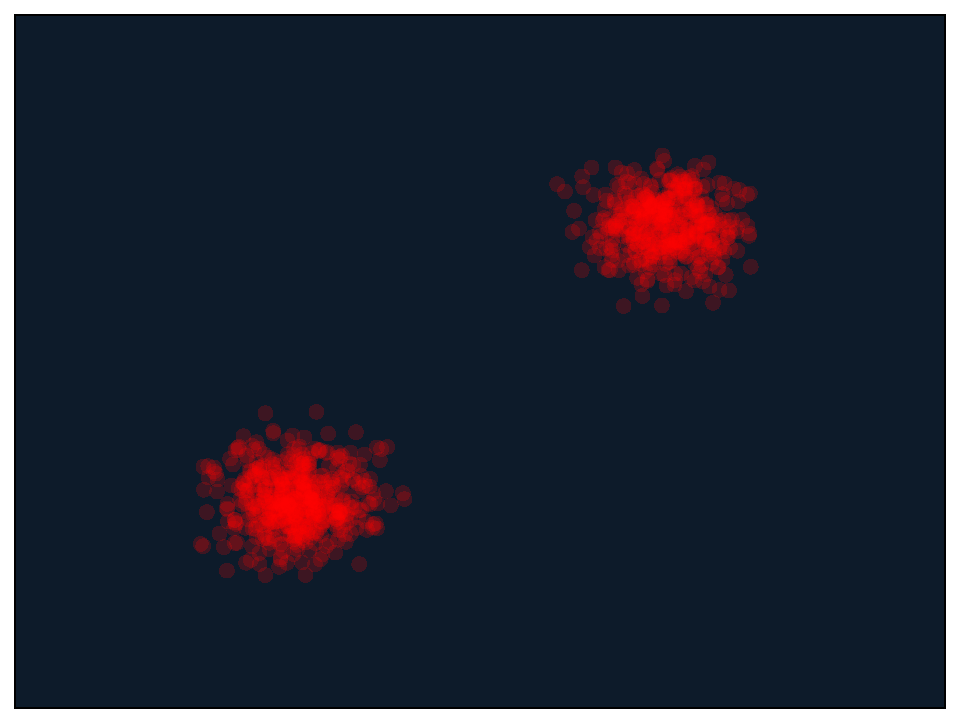
\includegraphics[width=.12\textwidth]{figures/concept_figure/distractors/posterior_gt} &
    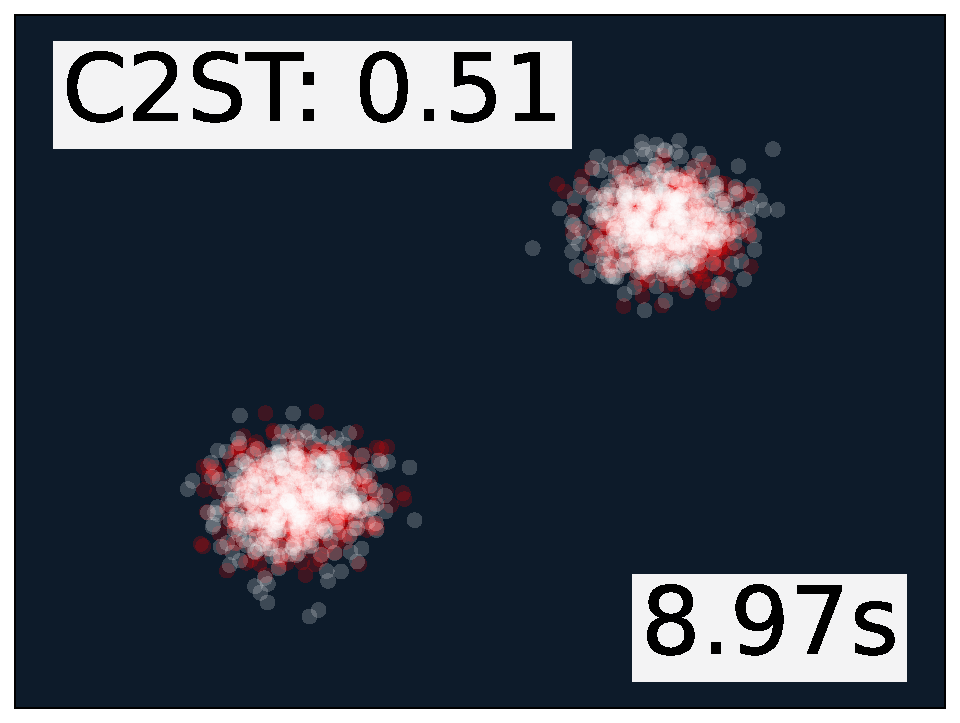
\includegraphics[width=.12\textwidth]{figures/concept_figure/distractors/posterior_r2omc_100} &
    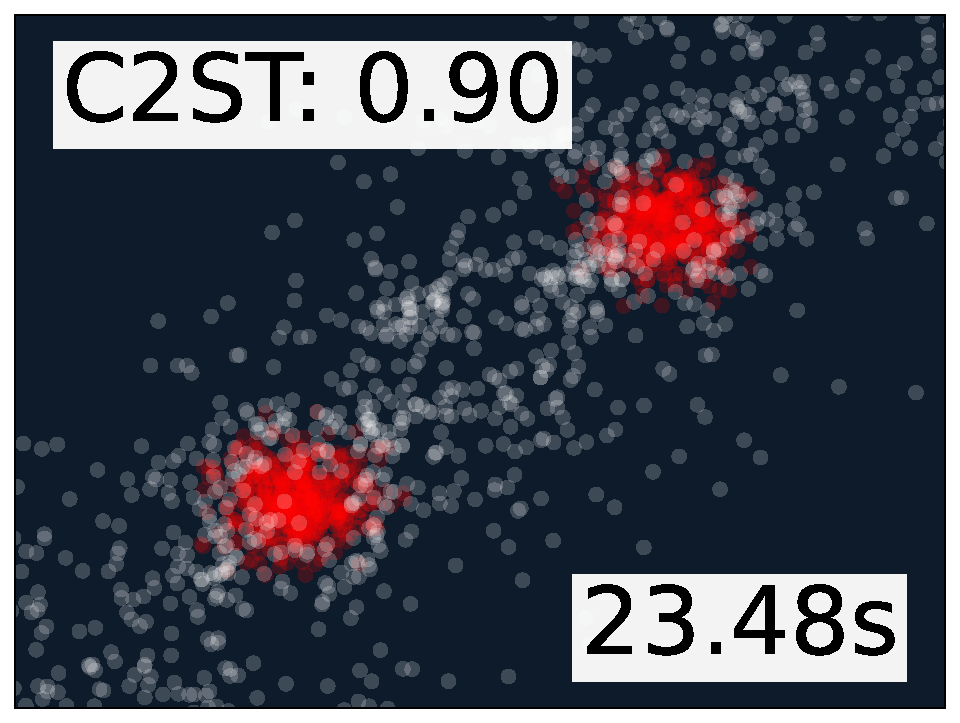
\includegraphics[width=.12\textwidth]{figures/concept_figure/distractors/posterior_npec_1000} &
    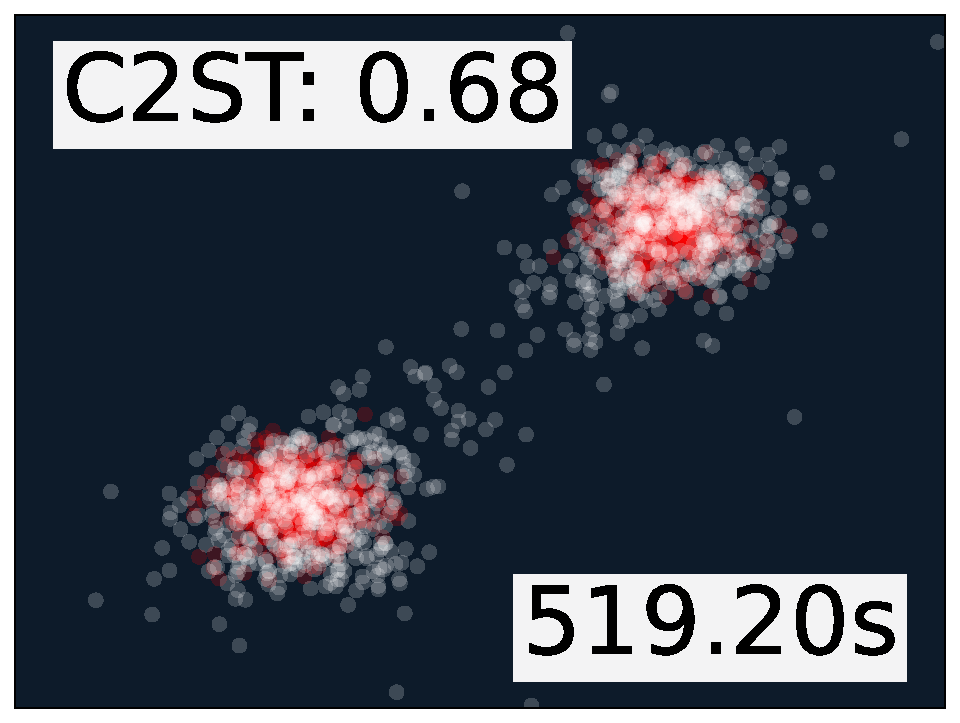
\includegraphics[width=.12\textwidth]{figures/concept_figure/distractors/posterior_npec_30000} &
    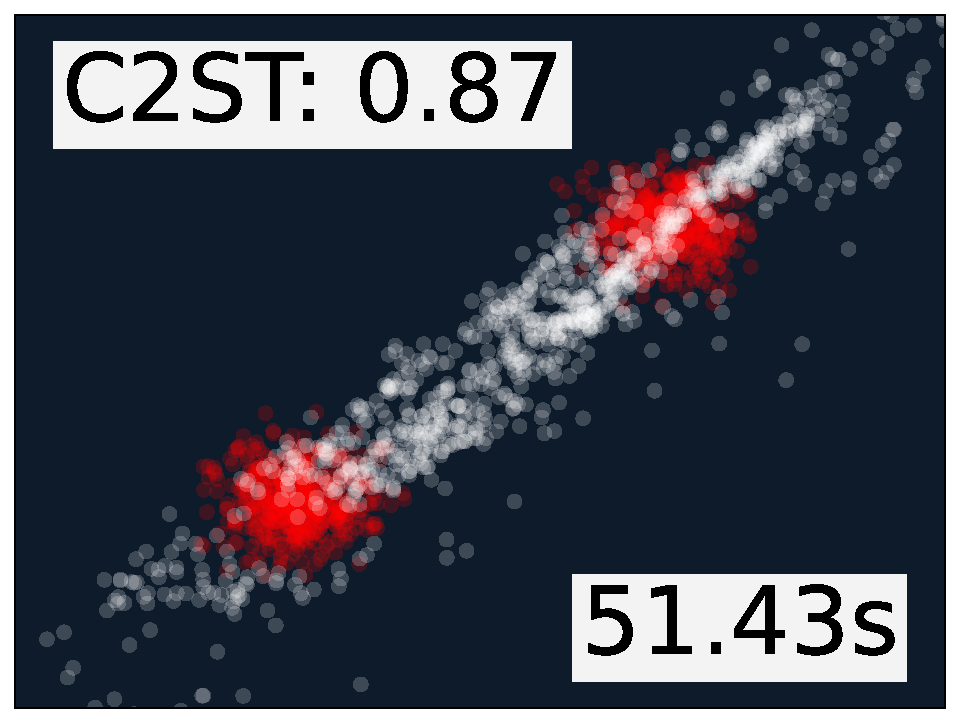
\includegraphics[width=.12\textwidth]{figures/concept_figure/distractors/posterior_bayes_flow_1000} &
    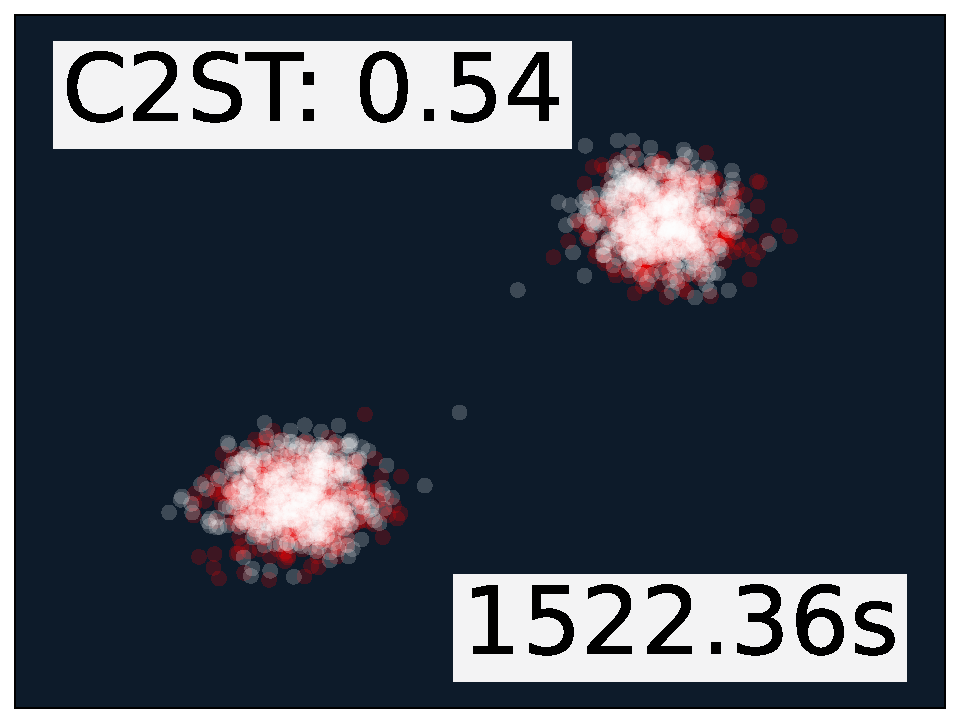
\includegraphics[width=.12\textwidth]{figures/concept_figure/distractors/posterior_bayes_flow_30000} &
    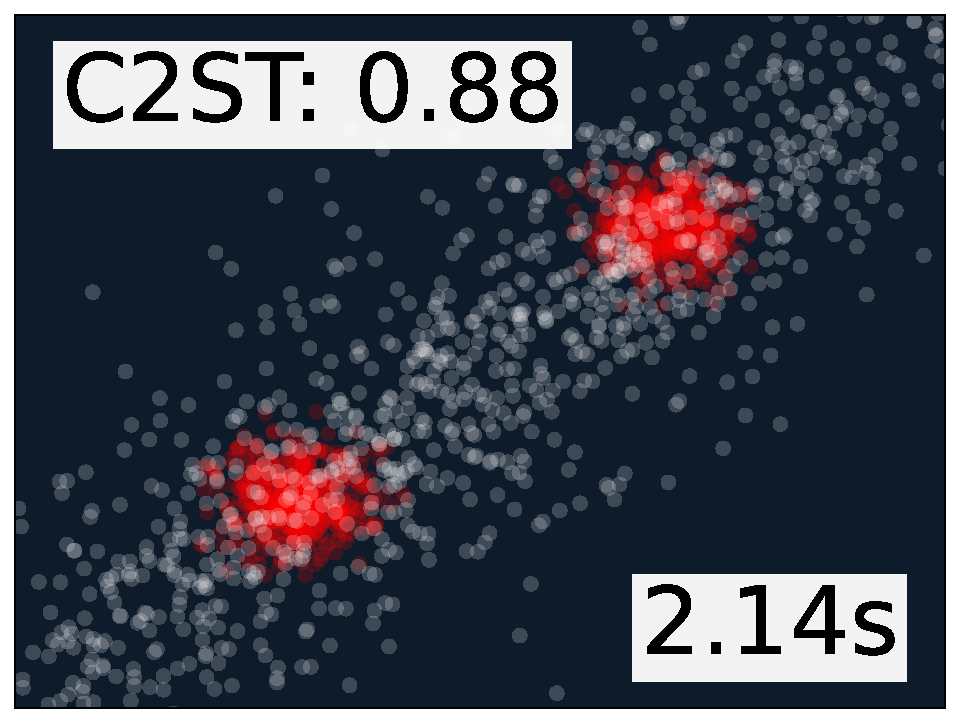
\includegraphics[width=.12\textwidth]{figures/concept_figure/distractors/posterior_flow_matching_1000} &
    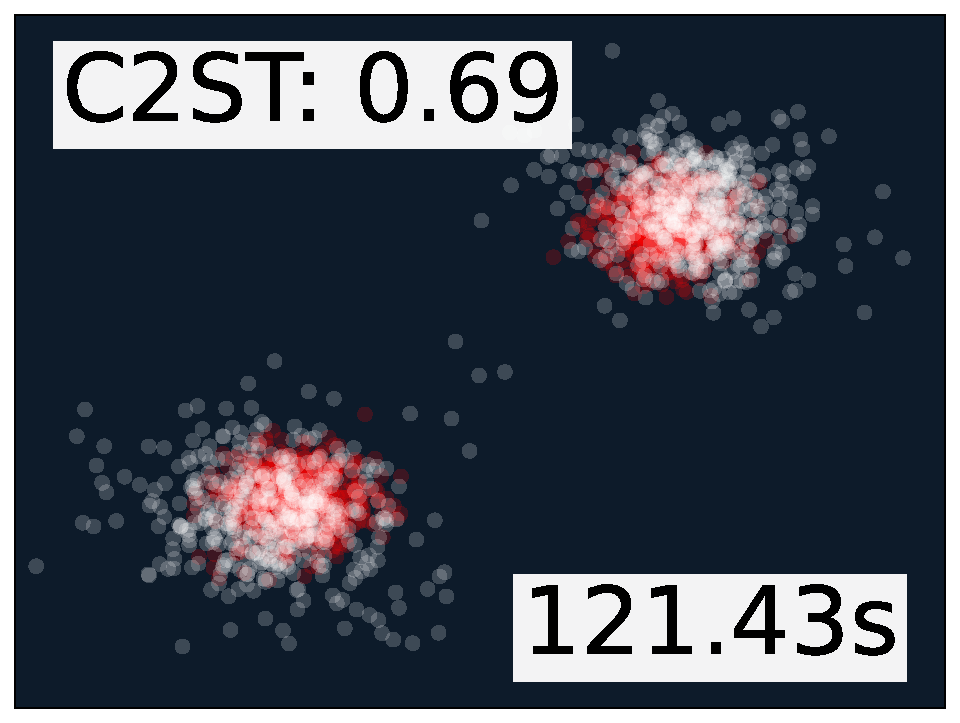
\includegraphics[width=.12\textwidth]{figures/concept_figure/distractors/posterior_flow_matching_30000} \\
    % Second row example
    \rotatebox{90}{\scriptsize{\; High-dim}} &
    
\includegraphics[width=.12\textwidth]{figures/concept_figure/high_dim/posterior_gt} &
    
\includegraphics[width=.12\textwidth]{figures/concept_figure/high_dim/posterior_r2omc_100} &
    
\includegraphics[width=.12\textwidth]{figures/concept_figure/high_dim/posterior_npec_1000} &
    
\includegraphics[width=.12\textwidth]{figures/concept_figure/high_dim/posterior_npec_30000} &
    
\includegraphics[width=.12\textwidth]{figures/concept_figure/high_dim/posterior_bayes_flow_1000} &
    
\includegraphics[width=.12\textwidth]{figures/concept_figure/high_dim/posterior_bayes_flow_30000} &
    
\includegraphics[width=.12\textwidth]{figures/concept_figure/high_dim/posterior_flow_matching_1000} &
    
\includegraphics[width=.12\textwidth]{figures/concept_figure/high_dim/posterior_flow_matching_30000} \\
  \end{tabular}
  \caption{Your figure caption here.}
  \label{fig:pixelwise}
\end{figure*}

% \begin{figure*}[ht]
%     % Row 1: 5 images
%     \centering
%     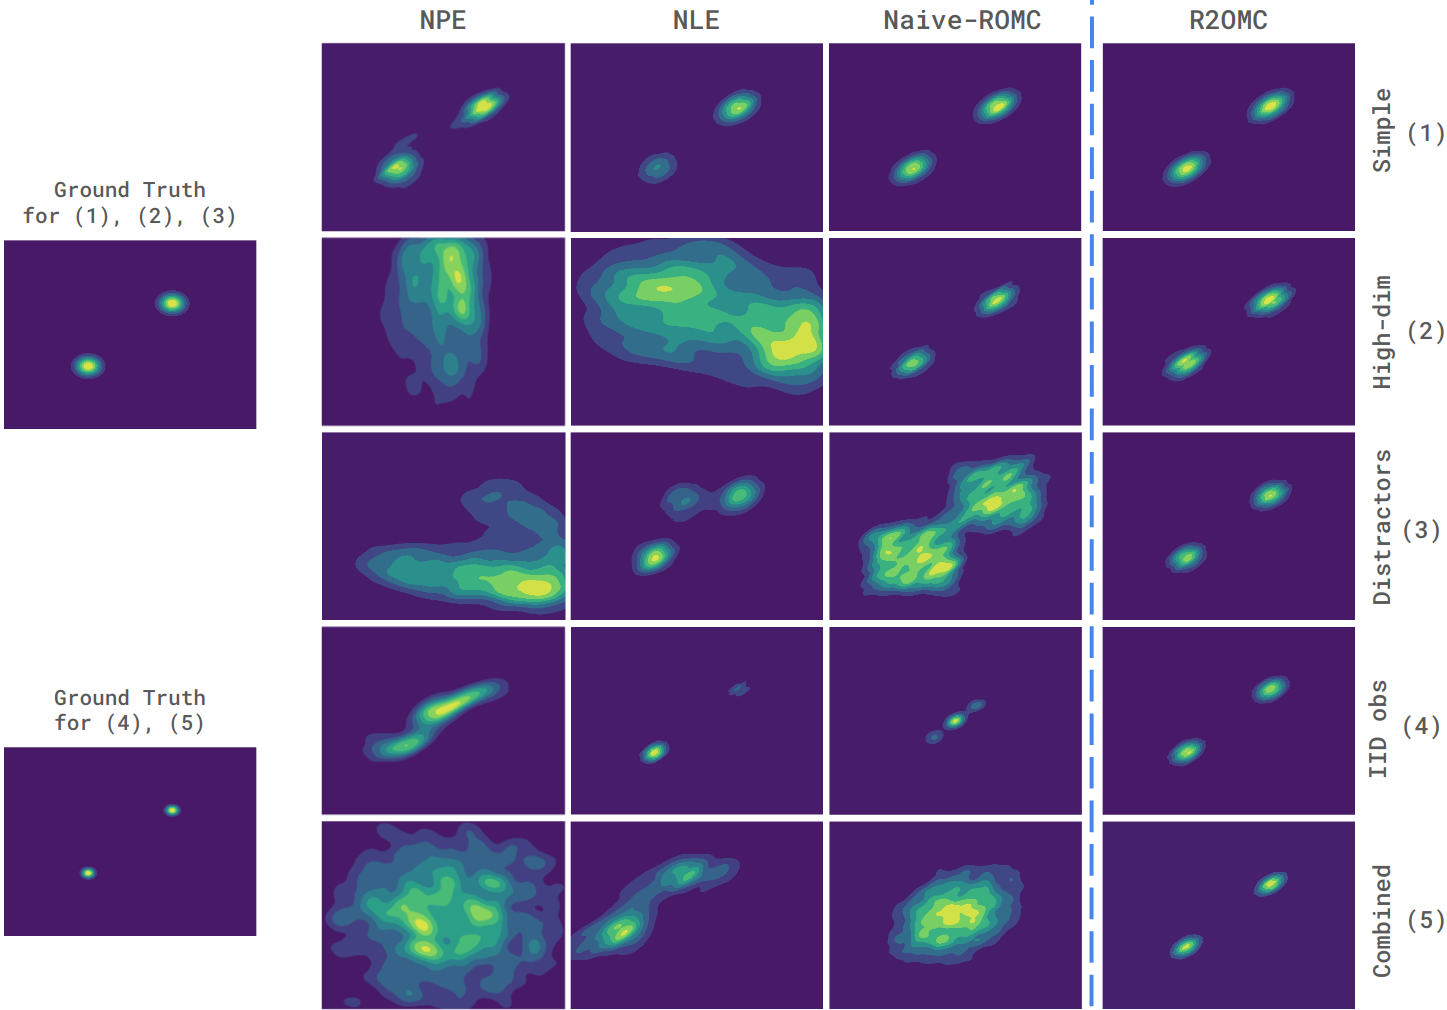
\includegraphics[width=1.\linewidth]{./figures/concept_example.png}
%   %\caption{Top to bottom: Simple, high-dimensional, distractors, multiple observations, combined. Left to right: ground truth, NPE, NLE, Naive-ROMC, R2OMC (proposed). Details in Section~\ref{app-sec:intro-example} of the Appendix.}
%   \caption{The simple setup (1) shows two-dimensional marginals for a five-dimensional inference problem, the high-dimensional setup (2) the same for a 20-dimensional problem. Distractors (3) add 10 uninformative dimensions to (1). (4) extends (1) to four iid observations. (5) combines (2-4). Details in Appendices \ref{app-sec:methods} and \ref{app-sec:intro-example}.}
%   \label{fig:concept_example}
% \end{figure*}

We here propose a new method that uses gradient information to deal with the above issues. We first convert the stochastic simulator to a set of deterministic simulators following the framework of Robust Optimization Monte Carlo~\citep[ROMC,][]{meeds2015optimization, ikonomov2020robust} and then use gradient-descent to efficiently obtain posterior samples. Very much like in standard optimization, the gradients are key to navigate the high-dimensional parameter space (Figure \ref{fig:concept_example}, columns 3-4). In addition, they allow us to perform sensitivity tests and filter out distractor dimensions, thereby improving the quality of the inference.

The ROMC framework provides the theory to convert posterior inference to deterministic optimization, which enables scalability to high-dimensional parameters, but is silent on the issues of multiple iid observations and the presence of distractors. In particular, it requires us to define a suitable distance function between simulated and observed data, and this becomes difficult with multiple observations or distractors.  Naive approaches can result in poor approximations of the posterior, as illustrated in  Figure ~\ref{fig:concept_example} (column 3, rows 3-5). Moreover, its  latest implementation~\citep{gkolemis2023extendable} does not exploit gradients and hence does not scale well to high-dimensional parameter dimensions. 

We here overcome these challenges, and introduce \rromc, an SBI method that belongs to the ROMC family of methods, which

\begin{itemize}
 \item enables high-dimensional gradient-based sampling from the posterior parameter distribution,
 \item handles multiple iid observations,
 \item automatically identifies and filters out uninformative dimensions (distractors),
 \item runs efficiently even for high-dimensional problems due to a \texttt{JAX} implementation that uses automatic differentiation, vectorization, and just-in-time compilation.
\end{itemize} 
\rromc~is systematically compared to state-of-the-art SBI methods. We find that it delivers accurate posterior samples at a fraction of the cost, even for problems where most SBI methods struggle.

\section{Background and Motivation}
We here briefly introduce Robust Optimization Monte Carlo (ROMC) and discuss the difficulties due to multiple iid\ data points and distractors.

\subsection{ROMC framework}
\label{subsec:ROMC}
ROMC has been introduced by \citet{ikonomov2020robust}, extending and addressing robustness issues of the Optimization Monte Carlo method by \citet{meeds2015optimization}. It belongs to the larger family of ABC methods that approximate the likelihood function as the probability of simulating an output $\epsilon$-close to the observation,
\begin{equation}
L_\epsilon(\thb) = \Pr(d(\yb, \data) \leq \epsilon \mid \thb).
\label{eq:abc_likelihood}
\end{equation}
Here, $d(\cdot, \cdot)$ is a distance, $\yb$ the simulator output, and $\data$ the observed data. In the following, we denote by $g(\thb, \ub)$ the simulator that maps noise (nuisance) variables $\ub \sim p(\ub)$\footnote{In a computer program, sampling $\ub$ corresponds to sampling a random seed.} and parameters $\thb$ to multivariate data $\yb = g(\thb, \ub)$. Introducing the acceptance region $C_\epsilon = \{(\thb, \ub): d(g(\thb, \ub), \data)\le \epsilon\}$ and using the law of the unconscious statistician, (\ref{eq:abc_likelihood}) can be written as
\begin{equation}
    L_\epsilon(\thb) = \E_{p(\ub)}\left[\mathbb{1}_{C_\epsilon}(\thb, \ub) \right],
\end{equation}
where $\mathbb{1}_{C_\epsilon}$ denotes the indicator function that is one if $(\thb, \ub)\in C_\epsilon$ and zero otherwise. When approximating the expectation as a sample average, we obtain
\begin{equation}
    L_\epsilon(\thb) \approx \frac{1}{S} \sum_{i=1}^S \mathbb{1}_{\accregioni}(\thb),
    \label{eq:omc_likelihood}
\end{equation}
which is the proportion of acceptance regions $\accregioni = \{\thb : d(g(\thb, \ub_i), \data) \leq \epsilon \}$ that contain $\thb$.

% \subsection{ABC and Rejection-ABC}

% ABC methods approximate the likelihood as the probability of simulating an output that is $\epsilon$-close to the observation.
% The ABC likelihood is $L_\epsilon(\thb) = \Pr(d(\yb, \data) \leq \epsilon)$, where $d(\cdot, \cdot)$ is a distance, $\yb$ the simulator's output, and $\data$ the observed data.
% For a prior $p(\thb)$ and a simulator $g(\thb, \ub)$, where $\thb$ are the parameters of interest and $\ub$ are the nuisance variables that control the randomness of the simulator, ABC posterior is:

% \begin{equation}
%     \label{eq:abc_posterior}
%     p_{\epsilon}(\thb | \data) \propto p(\thb) \Pr(d(g(\thb, \ub), \data) \leq \epsilon)
% \end{equation}


% Sampling from (\ref{eq:abc_posterior}) with a high acceptance rate while keeping the approximation error $\epsilon$ low is difficult.
% Rejection ABC samples many $\thb_i \sim p(\thb)$ and $\ub_i \sim p(\ub_i)$~\footnote{In a computer program, sampling $\ub_i \sim p(\ub)$ equals to sampling a seed from a discrete uniform distribution over all possible seeds, typically $1, \ldots, 2^{32} - 1$.},
% with the hope that some of them will produce an output $\yb_i = g(\thb_i, \ub_i)$ close to the observation, i.e., $d(\yb_i, \data) < \epsilon$, where $\epsilon$ is small.
% In high-dimensional problems, where a small proportion of the prior has high likelihood, $\epsilon$ must be increased to accept even a few $\thb_i$, leading to a high approximation error.

% \subsection{OMC and Robust OMC}

% OMC breakthrough is to sample $S$ nuisance variables $\{\ub_i\}_{i=1}^S$ from $p(\ub)$ and convert the probabilistic simulator $g(\thb, \ub)$ to a set of deterministic functions $\{g(\thb, \ub_i)\}_{i=1}^S$.
% Each $g(\thb, \ub_i)$ is associated with a set of $\thb$-points that generate outputs $\epsilon$-close to the observation, i.e., 
% an acceptance region $\accregioni = \{\thb : d(g(\thb, \ub_i), \data) \leq \epsilon \}$.
% OMC approximates the likelihood \textit{with the proportion of acceptance regions that contain $\thb$, i.e., $L_{\epsilon}(\thb) = \sfrac{1}{S} \sum_i^S \mathbb{1}_{\accregioni}(\thb)$,}
% where $\mathbb{1}_{\accregioni}(\thb) = 1$ if $d_i(\thb) \leq \epsilon$ and $0$ otherwise.
% OMC posterior is:

% \begin{equation}
%   \label{eq:omc_posterior}
%   p_{\epsilon}( \thb | \data) \propto p(\thb) \sum_i^S \mathbb{1}_{\accregioni}(\thb)
% \end{equation}

ROMC takes (\ref{eq:omc_likelihood}) as starting point and focuses on characterizing the acceptance regions $\accregioni$, because once the $\accregioni$ are known, we can not only evaluate the approximate likelihood function, but also obtain posterior samples efficiently. ROMC achieves this by introducing (uniform) proposal distributions $q_i$ with support on $\accregioni$ only. Samples from $\thb_{ij} \sim q_i$ for $j \in 1,\ldots, M$, are then equal to posterior samples if weighted with the (unnormalized) weights $w_{ij}$, $i=1, \ldots, S, j=1, \ldots, M$,
\begin{equation}
w_{ij} = \frac{p(\thb_{ij})}{q_i(\thb_{ij})} \mathbb{1}_{C^i_{\epsilon}}(\thb_{ij}) \label{eq:romc_weight}.
\end{equation}
% Omitted for space resaons. It may also distract from the story line. A reason to keep it would be that it explains what one can do with weighted samples, but this should clear to our readers, and comes up again later.
% Posterior expectations $\E[h(\thb) | \data]$, where $h$ is an arbitrary function, can then be approximated by
% \begin{equation}
% \label{eq:romc_posterior}
% \bar{h} = \frac{\sum_{i, j} w_{ij} h(\thb_{ij})}{\sum_{i,j} w_{ij}}.
% \end{equation}
For the characterization of the acceptance regions $\accregioni$, ROMC first determines the minimizers $\thb_i^*$,
\begin{equation}
 \thb_i^* = \text{argmin}_{\thb} d_i(\thb),\quad d_i(\thb) = d(g(\thb, \ub_i), \data),       
 \label{eq:optim_end_points}
\end{equation}
where $d_i(\thb)$ are deterministic distance functions because the sources of randomness (seed) are set to $\ub_i$ and kept fixed.
Next, it starts from the optimization end points $\thb_i^*$ to map out $\accregioni$ using for $\epsilon$ a value derived from the quantiles of the minimial distance functions, $d_i^*=d_i(\thb_i^*), i=1, \ldots, S$ \citep[see][for details]{ikonomov2020robust}. While several options are possible \citep{ikonomov2020robust}, we here use hyperboxes centered at $\thb_i^*$, which can be constructed with a line search algorithm for each parameter dimension. For details, please see Appendix \ref{app-sec:methods}.

The power of the ROMC framework stems from the possibility to use optimization, in particular gradient-based methods, to determine the optimization end points $\thb_i^*$, and hence the acceptance regions $\accregioni$ and the proposal distributions $q_i$. We will exploit this in our method to scale SBI to higher parameter dimensions. Before we can tap into the ROMC framework, however, we will need to overcome challenges related to the definition of the distance function $d$ in case of multiple iid observations and the presence of distractors.

% Based on (\ref{eq:omc_posterior}), ROMC proposed an importance sampling strategy that maintains a high acceptance rate, even when the problem is high-dimensional and $\epsilon$ is small.
% We present ROMC in Algorithm~\ref{alg:romc_algorithm}.
% The key idea is that the areas around the minimizers $\thb_i^* = \text{argmin}_{\thb} d_i(\thb)$ of the deterministic distance functions $d_i(\thb) = d(g(\thb, \ub_i), \data)$ are of high-likelihood, so they can be used as proposal regions.

% \begin{algorithm}[!ht]
%   \caption{\texttt{ROMC}. Requires: $p(\thb), g(\thb, \ub)$}
%   \label{alg:romc_algorithm}
%   \begin{algorithmic}[1]
%     \Procedure{ROMC}{$S, M, \epsilon$}
%       \For{$i \gets 1 \textrm{ to } S$}
%         \State{$\thb_i^* = \text{argmin}_{\thb} d_i(\thb)$, $d_i(\thb) = d(g(\thb, \ub_i), \data)$}
%         \State{\textbf{if} \(d^*_i(\thb) > \epsilon\) \textbf{then} reject and go to 2}
%         \State{Construct \(q_i\) based on Algorithm~\ref{alg:region_construction}}
%         \For{\(j \gets 1 \textrm{ to } M\)}
%           \State $\thb_{ij} \sim q_i$, $w_{ij} = \frac{p(\thb_{ij})}{q(\thb_{ij})} \mathbb{1}_{C^i_{\epsilon}}(\thb_{ij})$ 
%         \EndFor{}
%       \EndFor{}
%       \State{\Return{$\{ (\thb_{ij}, w_{ij}) \}_{i,j}$}}
%     \EndProcedure{}
%   \end{algorithmic}
% \end{algorithm}

% The minimizer $\thb_i^*$ can be found with any regular optimization technique, like gradient descent.
% A hyperbox of volume $V_i$ is constructed around it with a line search algorithm (Algorithm~\ref{alg:region_construction} of the Appendix) and serves as a uniform proposal distribution $q_i$. The hyperbox must enclose all the acceptance region, $C^i_{\epsilon}$, with the minimum redundant volume to avoid zero-likelihood regions.
% Finally, $M$ points are sampled from each $q_i$ and the expectation $\bar{h} = \E_{p_{\epsilon}}[h(\thb)]$ of an arbitrary function $h$ is approximated as:

% \begin{equation}
% \label{eq:romc_weight}
% \bar{h} = \frac{\sum_{i, j} w_{ij} h(\thb_{ij})}{\sum_{i,j} w_{ij}}, \: w_{ij} = \frac{p(\thb_{ij})}{q_i{\thb_{ij}}} \mathbb{1}_{C^i_{\epsilon}}(\thb_{ij})
% \end{equation}

\subsection{Challenges due to iid data and distractors}
\label{sec:romc-limitations}
The ROMC framework is silent on the choice of the distance function $d$. It assumes that a suitable one has been defined. However, poor choices can be detrimental to the posterior approximation. In particular, if the minimal distances $d_i^*$ remain too large for many seeds $i$ even after successful optimization, $\epsilon$ will be chosen too large and the posterior approximation will be too loose. We here highlight two important cases where defining a suitable distance function $d_i(\thb)$ is difficult, both in general and for ROMC in particular.

\paragraph{Multiple iid observations.}
Consider a simulator $\yb | \thb \sim 0.5\left ( \mathcal{N}(\thb, \mathbf{I}) + \mathcal{N}(-\thb, \mathbf{I}) \right )$, where $\thb \in \mathbb{R}^{10}$ are the parameters of interest, a uniform prior on $[-15, 15]^{10}$ for them, and $N=4$ iid observations. Let the first two observed data points $\data_{\{1,2\}} \approx (5, \ldots, 5)$ and the last two $\data_{\{3,4\}} \approx (-5, \ldots, -5)$.
The posterior for $\thb$ is approximately a truncated mixture of Gaussians whose components are centered at $(5, \ldots, 5)$ and $(-5, \ldots, -5)$ with a covariance matrix equal to $\mathbf{I}/4$ (see Appendix \ref{app-sec:intro-example}). 

A straightforward approach for defining the distance function is to run the simulator with different seeds $\ub_{i,n}$ for each observation $n$, and to average the per data-point distances so that $d_i(\thb) = 1/N \sum_n \tilde{d}(g(\thb, \ub_{i,n}), \data_n)$, where $\tilde{d}$ is a distance function for a single data point. However, this approach is sensitive to the ordering of the observations. The optimal distance $d_i^*$ approaches zero only when $\ub_{i,1}, \ub_{i,2}$ make the simulator generate data from the same mixture component, say $\mathcal{N}(\thb, \mathbf{I})$, and $\ub_{i,3}, \ub_{i,4}$ from the opposite one, say $\mathcal{N}(-\thb, \mathbf{I})$).
In all other scenarios, $d_i^*$ remains large, resulting in a large $\epsilon$ that leads to a posterior that is broader than the true posterior. This issue increases with the number of observations due to the factorial growth in possible permutations. Similar issues occur for other simple approaches such as concatenating all the iid data points  into a single vector. For squared Euclidean distances, the two approaches coincide.
Figure~\ref{fig:concept_example} illustrates the drop in performance of ROMC when averaging per-data point distances. %In Appendix (\ref{app-subsec:distance-iid}), we explore alternative distance measures, highlighting the limitations of most straightforward approaches.
% Some of them are quite complex, like learning permutation-invariant summary statistics. Other simple options, like generating one output and average the distance to all observations, may yield in even worse results.

\paragraph{Uninformative dimensions (distractors).}
\label{sec:romc-limitation-1}

We defined distractors to be output dimensions that do not relate to the parameters of interest. A concrete example is a graphics renderer where the parameter of interest controls a localized part of the scene, e.g.\ the appearance of vase, so that most pixel values of the scene are unrelated to the parameter. To emulate distractors, we consider a simulator $\yb = (\yb^{(1)}, \yb^{(2)})$, where the first set of dimensions $ \yb^{(1)} \sim 0.5 \left ( \mathcal{N}(\thb, \mathbf{I}) + \mathcal{N}(-\thb, \mathbf{I}) \right )$ and the second set of dimensions $\yb^{(2)} \sim \mathcal{N}(\boldsymbol{\mu}, 100\mathbf{I})$, where $\boldsymbol{\mu} \sim \mathcal{U}(-\mathbf{10}, \mathbf{10})$. Note that only $\yb^{(1)}$ depends on $\thb$; $\yb^{(2)}$ represents distractors.
Given one observation $\data = (\yb^{o, (1)}, \yb^{o, (2)})$, with $\yb^{o, (1)} \approx (5, \ldots, 5)$, and for $\thb$ a uniform prior on $[-15, 15]^D$ as before, the posterior is solely influenced by $\yb^{o, (1)}$. It is approximately equal to a truncated mixture of two Gaussians with components centered at $(5, \ldots, 5)$ and $(-5, \ldots, -5)$, each having an identity covariance matrix, see Appendix \ref{app-sec:intro-example}. Since $\yb^{(2)}$ does not depend on $\thb$, the minimal distances $d_i^*$ will generally be large for seeds that generate an output $\yb^{(2)}$ significantly different from $\yb^{o, (2)}$.
This results in a large $\epsilon$, which again leads to a posterior that is much broader than the true posterior. Figure~\ref{fig:concept_example} visualizes how ROMC is affected by distances that are sensitive to distractors.

\section{Proposed method: \rromc}
\label{sec:rromc}
We here present our new method for Bayesian parameter inference in simulator models. The method uses gradients to obtain posterior samples even in high-dimensional parameter spaces. The method belongs to the ROMC framework so that we start with discussing how we deal with iid observations and distractors before discussing its implementation.
\begin{figure*}[!ht]
  \centering
  
\includegraphics[width=\linewidth]{./figures/concept_image.png}
  \caption{
    Overview \rromc: Distractors are automatically filtered out and proposal distributions $q_i^n$ are created for each observation (here two): the blue-dotted region indicates where the proposal distributions for the first observation are nonzero, and the green-dotted region indicates the same for the second observation. Only samples that fall within the intersection of both regions are given a positive weight and become posterior samples.}
  \label{fig:concept_image}
\end{figure*}

\subsection{Multiple iid observations}
\label{subsec:multiple-observations}
The likelihood for multiple iid observations $\{\data_n\}_{n=1}^N$ is the product of the likelihoods for each data point. Approximating the likelihood for each data point as in (\ref{eq:omc_likelihood}) and multiplying-in the prior $p(\thb)$, we can obtain a formal expression for the approximate posterior
\begin{equation}
  \label{eq:rromc_posterior}
  p_{\epsilon}(\thb | \{\data_n\}) \propto p(\thb) \prod_{n}^{N} \sum_{i}^S \mathbb{1}_{C_{\epsilon}^{i,n}}(\thb),
\end{equation}
where $C_{\epsilon}^{i,n}$ is the acceptance region for data point $n$ and source of randomness (seed) $\ub_{i,n}$,
\begin{equation}
C_{\epsilon}^{i,n} = \{\thb : d(g(\thb, \ub_{i,n}), \data_n) \leq \epsilon \}.
\end{equation}
We have $S$ sources of randomness for each data point $\data_n$, and so in total $S*N$ acceptance regions $C_{\epsilon}^{i,n}$.

We now address the question how to efficiently sample from $p_{\epsilon}(\thb | \{\data_n\})$. To achieve this, we consider the task of computing the posterior expectation $\bar{h} = \E_{p_{\epsilon}}[h(\thb)]$ under $p_{\epsilon}(\thb | \{\data_n\})$. Plugging in the expression in (\ref{eq:rromc_posterior}) gives, after normalization,
\begin{equation}
  \label{eq:rromc_expectation}
  \bar{h} = \frac{ \int h(\thb) p(\thb) \prod_n^N \sum_i^S \mathbb{1}_{C_{\epsilon}^{i,n}}(\thb) d\thb}{\int p(\thb) \prod_n^N \sum_i^S \mathbb{1}_{C_{\epsilon}^{i,n}}(\thb) d\thb}.
\end{equation}
%
%
% We derive the ABC posterior for iid observations $\{\data_n\}_{n=1}^N$. Let $L_{\epsilon}^n(\thb)$ be the ABC likelihood for the $n$-th observation and $L_{\epsilon}(\thb)$ the joint likelihood. Due to iid, $L_{\epsilon}(\thb) = \prod_{n}^{N} L_{\epsilon}^n(\thb)$ and the ABC posterior is:
% \begin{equation}
%   \label{eq:joint-ABC}
%   p(\thb | \{\data_n\}_n) \propto p(\thb) \prod_{n}^{N} \Pr(d(g(\thb, \ub), \data_n) \leq \epsilon)
% \end{equation}
% % Eq.~(\ref{eq:joint-ABC}) generalizes (\ref{eq:abc_posterior}) to multiple observations.
% Each $L_{\epsilon}^n(\thb)$ can be approximated using $S$ different seeds;
% let $\ub_{i,n}$ be the $i$-th seed of the $n$-th observation wich defines the distance function $d_i^n(\thb) = d(g(\thb, \ub_{i,n}), \data_n)$.
% The OMC-posterior for $N$ iid observations is defined through $S * N$ distances, each corresponding to an acceptance region $C_{\epsilon}^{i,n} = \{\thb : d(g(\thb, \ub_{i,n}), \data_n) \leq \epsilon \}$:

% \begin{equation}
%   \label{eq:rromc_posterior}
%   p_{\epsilon}(\thb | \{\data_n\}) \propto p(\thb) \prod_{n}^{N} \sum_{i}^S \mathbb{1}_{C_{\epsilon}^{i,n}}(\thb)
%   % \quad \text{where}
%   % \quad \mathbb{1}_{C_{\epsilon}^{i,n}}(\thb) = \begin{cases} 1 & \text{if } d(g(\thb, \ub_{i,n}), \data_n) \leq \epsilon \\ 0 & \text{otherwise} \end{cases}
% \end{equation}

% where $\mathbb{1}_{C_{\epsilon}^{i,n}}(\thb) = 1$ if $d(g(\thb, \ub_{i,n}), \data_n) \leq \epsilon$ and $0$ otherwise.
% Eq.~(\ref{eq:rromc_posterior}) is a direct consequence of (\ref{eq:omc_posterior}) and (\ref{eq:joint-ABC}) and is a Monte Carlo approximation of (\ref{eq:joint-ABC}) with $S * N$ deterministic functions.

% The task is to efficiently sample from it and compute any expectation $\bar{h} = \E_{p_{\epsilon}}[h(\thb)]$:
% \begin{equation}
%   \label{eq:rromc_expectation}
%   \bar{h} = \frac{ \int h(\thb) p(\thb) \prod_n^N \sum_i^S \mathbb{1}_{C_{\epsilon}^{i,n}}(\thb) d\thb}{\int p(\thb) \prod_n^N \sum_i^S \mathbb{1}_{C_{\epsilon}^{i,n}}(\thb) d\thb}
% \end{equation}
The integrals in the equation are typically intractable. But they correspond to expectations with respect to the prior $p(\thb)$ and hence could be approximated with a sample average. However, this is very inefficient. Few (or no) prior samples will generate outputs $\epsilon$-close to all observations, so most (or all) will get zero weight, leading to a very low effective sample size. Following the general ROMC framework by \citet{ikonomov2020robust}, we thus employ importance sampling with an adaptive proposal distribution obtained via optimization. 

We first treat each data point $\data_n$ separately and construct proposal distributions $q_i^n(\thb)$, $i=1, \ldots, S$, as in Section \ref{subsec:ROMC}: We use optimization to find the minimizers $\thb_{i,n}^*$ of the deterministic functions $d_i^n(\thb) = d(g(\thb, \ub_{i,n}), \data_n)$,       
\begin{equation}
 \thb_{i,n}^* = \text{argmin}_{\thb} d_i^n(\thb),
 \label{eq:rromc_optim_end_points}
\end{equation}
and then build a hyperbox around each acceptance region $C_{\epsilon}^{i,n}$ and define $q_i^n(\thb)$ to be the uniform distribution over it. The optimization problem in (\ref{eq:rromc_optim_end_points}) is deterministic and we solve it with gradient-based methods to enable scalability to large parameter spaces. Note that treating each data point $\data_n$ separately allows us to avoid the issues explained in Section \ref{sec:romc-limitations}.

We propose to combine the per-data point proposal distributions $q_i^n(\thb)$ in form of a mixture distribution,
\begin{equation}
    q(\thb) = \frac{1}{N} \frac{1}{S} \sum_{n=1}^N \sum_{i=1}^S q_i^n (\thb).
    \label{eq:R2OMC-proposal}
\end{equation}
The posterior expectation in (\ref{eq:rromc_expectation}) can then be approximated in form of a weighted average 
\begin{equation}
  \label{eq:rromc_sample_expectation}
  \bar{h} = \frac{\sum_p w_p h(\thb_p)}{\sum_p w_p}, \quad \thb_p \sim q(\thb)
\end{equation}
where the weights $w_p$, $p=1, \ldots, P$, are given by
\begin{equation}
  \label{eq:rromc_weight}
w_p= \frac{p(\thb_p)}{q(\thb_p)} \prod_{n=1}^N \sum_{i=1}^S \mathbb{1}_{C_{\epsilon}^{i,n}}(\thb_p). 
\end{equation}
This means that the $\thb_p \sim q(\thb)$, weighted by $w_p$, represent samples from the posterior $p_{\epsilon}(\thb | \{\data_n\})$ in (\ref{eq:rromc_posterior}).

The rationale for choosing $q(\thb)$ in (\ref{eq:R2OMC-proposal}) as proposal distribution is as follows: it is a mixture of uniform distributions, so sampling and evaluating is easy. It seamlessly combines the contribution from multiple data points, allowing future data points to be included without re-computation. If each $q_i^n$ encloses the corresponding acceptance region $C_{\epsilon}^{i,n}$, then $q(\thb) > 0$ in areas of the parameter space where $\prod_n^N \sum_i^S \mathbb{1}_{C_{\epsilon}^{i,n}}(\thb) > 0$ and no posterior mass is discarded in the weighting in (\ref{eq:rromc_weight}). Finally, regions of high likelihood are characterized by regions where multiple $C_{\epsilon}^{i,n}$ overlap. As the proposal distribution $q(\thb)$ consists of a mixture of the $q_i^n(\thb)$ with equal weights, areas where multiple $C_{\epsilon}^{i,n}$ overlap will be sampled more often, so that areas of high likelihood will be represented with more samples.

Figure~\ref{fig:concept_image}, steps (ii-iii), illustrates the proposed procedure to obtain posterior samples. We have two observed data points and the $\thb_p$ come from regions that match at least one observation; the blue-dotted area for $\data_1$ and the green-dotted region for $\data_2$. However, only the ones that match both will get a positive weight (red dots) and become posterior samples.
% If the per-observation acceptance regions have little (or no) overlap, i.e. $\bigcap_n^N \bigcup_i^S C_{\epsilon}^{i,n}(\thb)$ is small (or empty), the acceptance rate will drop or even become zero.
% In this case, we may use a higher $\epsilon$ threshold, but if the problem persists, it is
% an alarm about possible model-misspecification; there are no parameter values that can match all observations.

% Finally, note that~(\ref{eq:rromc_weight}) holds independently of a specific $q$.
% The main \rromc~algorithm (Algorithm~\ref{alg:r2omc}, repeatedly calls the \texttt{CoreR2OMC} algorithm (Algorithm~\ref{alg:core_r2omc}) for building the per-observation proposal regions.
% Therefore, if a more efficient or accurate proposal region algorithm is developed, it can be easily integrated into \rromc~framework.

\subsection{Uninformative dimensions (distractors)}
\label{subsec:distractors}
Distractors can negatively affect the quality of the posterior approximation. To counteract their influence, we measure the sensitivity of the output dimensions with respect to the parameters $\thb$ by computing the average norm of their derivative with respect to $\thb$, and checking that the value is above a minimal value (threshold) $\tau$, 
\begin{equation}
  \label{eq:informative_dimensions}
  I_i = \E_{p(\thb)p(\ub)}\left[ || \nabla_{\thb} g_i(\thb, \ub) || \right] > \tau.
\end{equation}
The expectation equals the expectation with respect to the joint distribution of the prior and the $i$-th dimension of the simulator output, $g_i(\thb, \ub)$. In our experiments, we approximate the expectation using $50$ samples from $p(\thb)$ and $p(\ub)$ each. Collecting all binary indicator variables $I_i$ into the vector $\mask$, we can filter out uniformative dimensions by computing the distance between observed and simulated data for informative dimensions only. To compute $\thb_{i,n}^*$ in (\ref{eq:rromc_optim_end_points}), we minimize
\begin{equation}
d_i^n(\thb) = d(g(\thb, \ub_{i,n})\odot \mask, \data_n \odot \mask).
\label{eq:rromc-masked-distance}
\end{equation}
The procedure is illustrated in Figure~\ref{fig:concept_image}, step (i). 

The threshold $\tau$ controls the sensitivity of the test. In our experiments, we set $\tau$ to machine precision; more sophisticated approaches consist in monitoring the distribution of the expected norm of the gradient, or by assessing false vs true positives under control conditions. This is possible since the mask $\mask$ can be computed prior to receiving observed data.

% \rromc~includes a filtering step (Step (i) in Figure~\ref{fig:concept_image}) to identify and eliminate output dimensions that are not relevant to the parameters of interest. A binary mask \( I = (I_1, \ldots, I_{D_{\yb}}) \) is created, where \( I_i \) represents the \( i \)-th output dimension. This mask is computed using the gradients of the output dimensions with respect to the parameters of interest:

% \begin{equation}
%   \label{eq:informative_dimensions}
%   I_i = \left( \frac{1}{L} \frac{1}{M} \sum_{l=1}^L \sum_{m=1}^M || \nabla_{\thb} g_i(\thb_l, \ub_m) || \right) > \tau
% \end{equation}

% where \( \thb_l \sim p(\thb) \), \( \ub_m \sim p(\ub) \) and \( \nabla_{\thb} g_i(\thb_l, \ub_m) \) is the gradient of the \( i \)-th output dimension wrt each parameter \( \thb_j \), i.e., \( ( \sfrac{\partial g_i(\thb_l, \ub_m)}{\partial \thb_1}, \ldots, \sfrac{\partial g_i(\thb_l, \ub_m)}{\partial \thb_D} ) \). 
% If the sum of the gradient norms is below the threshold \( \tau \), the \( i \)-th output dimension is deemed uninformative, resulting in \( I_i = 0 \). The gradients are calculated over \( L \) parameter values \( \thb_l \) and \( M \) seeds \( \ub_m \), where both \( L \) and \( M \) can be adjusted by the user. In our experiments, we set both values to 50. This process is repeated for all output dimensions, producing the binary vector \( I \). The distance function is then defined as \( d(\yb \odot I, \data \odot I) \).
% The threshold \( \tau \) is a hyperparameter that controls the sensitivity of the test. In our experiments, we set \( \tau = 0 \), meaning that all gradients must be zero for an output dimension to be considered uninformative; however, users can modify it to a less strict value.

\subsection{\texttt{JAX} implementation}
\label{subsec:implementation}

Algorithms~\ref{alg:r2omc} summarizes the key steps of \rromc. It has three steps: dealing with distractors (line 2); constructing per-data point proposal distributions $\{q_i^n\}_{i=1}^S$ (lines 4-5); combining them to form the overall proposal distribution $q(\thb)$ and generating the weighted samples (lines 7-8).

\begin{algorithm}[!ht]
  \caption{\texttt{R2OMC}. Requires: $p(\thb), g(\thb, \ub), \{\data_n\}_{n=1}^{N}$}
  \label{alg:r2omc}
  \begin{algorithmic}[1]
    \Procedure{\rromc}{$\tau, S, P$}
      \State $\mask = (I_1, \ldots, I_{D_{y}})$ using~(\ref{eq:informative_dimensions}) with $\tau$ 
      \For{\(n \gets 1 \textrm{ to } N\)}
      \State $\thb_{i,n}^* = \text{argmin}_{\thb} d_i^n(\thb)$ using (\ref{eq:rromc-masked-distance}) for all $i$
      \State Compute hyperboxes and $\{q_i^n\}_{i=1}^S$
    \EndFor
    \State $\thb_p \sim q(\thb)$, where $ q(\thb)= \frac{1}{N} \frac{1}{S} \sum_n \sum_i q_i^n (\thb)$
    \State Compute $\{w_p\}_p^P $ using (\ref{eq:rromc_weight})
    \State \Return $\{w_p, \thb_p\}_{p=1}^{P}$ 
    \EndProcedure
  \end{algorithmic}
\end{algorithm}

We offer an efficient \texttt{JAX} implementation, benefiting from automatic differentiation (\texttt{grad}), vectorization (\texttt{vmap}), and just-in-time compilation (\texttt{jit}). 
In many cases, \rromc~executes in seconds where most SBI methods require minutes (see Section~\ref{sec:experiments}). 

\rromc~requires approximately $N * S$ evaluations of the simulator: For the distractors, \texttt{grad} computes $\partial g_i/\partial \theta_j$ for all $i$ and $j$ in one call, and \texttt{vmap} evaluates multiple $\thb$ at once.
Combining them, the cost is $S$. Obtaining the per-data point proposal distributions $\{q_i^n\}_{i=1}^S$ consists of optimization (line 4) and hyperbox building (line 5) for each data point. Each of $S$ optimizations requires $T$ gradient descent steps, where $T$ is a user-defined hyperparameter. \texttt{jit} allows compiling $T_1$ consequtive steps to apply them at the cost of a single execution, so the cost reduces to $S \frac{T}{T_1}$. $\frac{T}{T_1}$ is normally small, and can even reach $1$ if memory allows setting $T_1 = T$. Hyperbox building also requires of the order of $S$ steps when the required line searches are parallelized over each parameter dimensions using \texttt{vmap} (see Appendix \ref{app-sec:methods}). Thus the total cost of this step is of the order of $N*S$. For generating the weighted samples, (\ref{eq:rromc_weight}) is evaluated on $P$ samples (line 8).
The simulator is only used for computing $\prod_n^N \sum_i^S \mathbb{1}_{C_{\epsilon}^{i,n}}(\thb_p)$ which requires evaluating $S * N$ different distance functions on $P$ points each. Using \texttt{vmap} in each distance function, the total cost is $S * N$. Evaluating $q(\cdot)$ and $p(\cdot)$ does not require calling the simulator. Finally, if the simulator is expensive, the $S *N$ cost of checking whether the samples are in the acceptance regions can be avoided by using the hyperbox or another model for the acceptance region, see \citet{ikonomov2020robust}. 

The code is available at \LinkToCode.


% \subsection{\rromc~algorithm}
% \label{subsec:rromc_algorithm}

% \rromc~is presented in Algorithms~\ref{alg:r2omc} and~\ref{alg:core_r2omc}.

% \textbf{Algorithm~\ref{alg:r2omc} (\texttt{R2OMC})}:
% Performs the inference and returns the weighted posterior samples. It
% identifies the informative dimensions (Step 2) using (\ref{eq:informative_dimensions}), 
% applies \texttt{CoreR2OMC} (Algorithm~\ref{alg:core_r2omc}) to define the per observation proposal regions (Steps 3-5),
% defines the proposal distribution $q(\thb)$ (Step 6)
% and computes the weighted samples (Steps 7-8) using (\ref{eq:rromc_weight}).

% \textbf{Algorithm~\ref{alg:core_r2omc} (\texttt{CoreR2OMC})}:
% Creates the proposal regions for a single observation.
% For each seed, it finds the optimal $\thb_i^*$ that minimizes $d(g(\thb, \ub_i) \odot \mask, \data \odot \mask)$ (Step 4), and if it is $\epsilon_1$-close to the observation, it builds a hyperbox around it (Step 6) using Algorithm~\ref{alg:region_construction} provided in the appendix.
% % The algorithm is similar to ROMC.
% % The only difference is the use of the mask $I$ and the two $\epsilon$ thresholds:
% % $\epsilon_1$ for accepting a solution and $\epsilon_2$ for constructing the hyperbox, where $\epsilon_1 < \epsilon_2$.

% \begin{algorithm}[!ht]
%   \caption{\texttt{R2OMC}. Requires: $p(\thb), g(\thb, \ub), \{\data_n\}_{n=1}^{N}$}
%   \label{alg:r2omc}
%   \begin{algorithmic}[1]
%     \Procedure{\rromc}{$\tau, S, \epsilon_1, \epsilon_2, \epsilon_3, \eta, R, L, P$}
%       \State $\mask = (I_1, \ldots, I_{D_{y}})$ using~(\ref{eq:informative_dimensions}) with $\tau$ 
%       \For{\(n \gets 1 \textrm{ to } N\)}
%       \State $\{q_i^n\}_i^S \leftarrow$ Algorithm~\ref{alg:core_r2omc} with $\data_n, S, \epsilon_1, \epsilon_2$
%     \EndFor
%     \State $\thb_p \sim q(\thb)$, where $ q(\thb)= \frac{1}{N} \frac{1}{S} \sum_n \sum_i q_i^n (\thb)$
%     \State Compute $\{w_p\}_p^P $ using Eq.~\ref{eq:rromc_weight} with $\epsilon_3$
%     \State \Return $\{w_p, \thb_p\}_{p=1}^{P}$ 
%     \EndProcedure
%   \end{algorithmic}
% \end{algorithm}

% \begin{algorithm}[!ht]
%   \caption{\texttt{CoreR2OMC}. Requires: $p(\thb), g(\thb, \ub), \data, \mask$}
%   \label{alg:core_r2omc}
%   \begin{algorithmic}[1]
%     \Procedure{CoreR2OMC}{$S, \epsilon_1, \epsilon_2, \eta, R, L$}
%       \For{\(i \gets 1 \textrm{ to } S\)}
%         \State{$\ub_i \sim p(\ub)$}
%         \State{$\thb_i^* = \text{argmin}_{\thb} d(g(\thb, \ub_i) \odot \mask, \data \odot \mask)$}
%         \State{\text{if} {$d^*_i (\thb) > \epsilon_1$} \textbf{then} go to line 2}
%         \State{$q_i$ around $\thb_i^*$ with Alg.~\ref{alg:region_construction} using $\eta, R, L, \epsilon_2$}
%       \EndFor
%       \State \Return $\{q_i\}_{i}^{S}$
%     \EndProcedure
%   \end{algorithmic}
% \end{algorithm}

% \subsection{Implementation and Efficiency}
% \label{subsec:implementation}
% We offer an efficient \texttt{JAX} implementation of $\rromc$, benefiting from automatic differentiation (\texttt{grad}), vectorization (\texttt{vmap}), and just-in-time compilation (\texttt{jit}). 
% In many cases, \rromc~executes in seconds where most SBI methods require minutes (see Section~\ref{sec:experiments}).
% % \rromc~cost equals approximately $N * S$ evaluations of the simulator, which is affordable given that $N$ is small in most SBI problems. Even if $N$ is large, $S$ can be decreased to balance the cost.

% % \rromc~is very efficient due to its implementation in \texttt{JAX}, which offers automatic differentiation (\texttt{grad}), vectorization (\texttt{vmap}), and just-in-time compilation (\texttt{jit}). In many cases, \rromc~executes in seconds where most SBI methods require some minutes (see Section~\ref{sec:experiments} and Appendix~\ref{app-subsec:runtime}).
% % \rromc~cost equals approximately $N * S$ evaluations of the simulator, which is affordable given that $N$ is small in most SBI problems. Even if $N$ is large, $S$ can be decreased to balance the cost.

% Algorithm~\ref{alg:r2omc} hast three parts; distractors (Step 2), proposal regions (Steps 3-5) and weighted samples (Steps 6-8).
% For the distractors, \texttt{grad} computes $\partial g_i/\partial \thb_j$ for all $i$ and $j$ in one call, and \texttt{vmap} evaluates multiple $\thb$ at once.
% Combining them, the cost is $S$.
% For candidate samples (Steps 3-5), the cost is $N$ executions of \texttt{CoreR2OMC}, so $N*S$.
% For computing weights (Steps 6-8), (\ref{eq:rromc_weight}) is evaluated on $P$ samples.
% The simulator is only used for computing $\prod_n^N \sum_i^S \mathbb{1}_{C_{\epsilon}^{i,n}}(\thb_p)$ which requires evaluating $S * N$ different distance functions on $P$ points each. Using \texttt{vmap} in each distance function, the total cost is $S * N$. Evaluating $q(\cdot)$ and $p(\cdot)$ does not require calling the simulator. If the simulator is expensive, the $S *N$ cost of checking whether the samples are in the acceptance regions can be avoided by using the hyperbox or another model for the acceptance region, see \citet{ikonomov2020robust}.

% Algorithm~\ref{alg:core_r2omc} has two expensive steps: optimization (Step 4) and hyperbox building (Step 6).
% Optimization requires $T$ gradient descent steps, where $T$ is a user-defined hyperparameter.
% \texttt{jit} allows compiling $T_1$ consequtive steps to apply them at the cost of a single execution, so the cost reduces to $S \frac{T}{T_1}$.
% $\frac{T}{T_1}$ is normally small, and can even reach $1$ if memory allows setting $T_1 = T$.
% Hyperboxes require, for each axis and each seed, $2L+1$ query points and up to $R$ refinements (see Appendix).
% The $(2L+1) * D$ query points can be evaluated in a single call (using \texttt{vmap}), limiting the cost to $S*R$.
% In most cases, $R$ can be set to a small value (or even $1$).
% The total cost of \texttt{CoreR2OMC} is $S (\frac{T}{T_1} + R)$, which is approximately $S$.

\section{Experiments}
\label{sec:experiments}

We report simulation results on a Mixture of Gaussians (MoG) benchmark in Section~\ref{subsec:gaussian} and the SBI  benchmark by \citet{lueckmann2021benchmarking} in Section~\ref{subsec:sbi-benchmark}.
The MoG benchmark thoroughly evaluates methods under high-dimensionality, distractors and multiple observations.
SBI considers popular test simulators.

\paragraph{Methods.}
In the MoG benchmark, we compare \rromc~with a straightforward use of the \romc~framework (\nromc) and two neural methods: \NPE~\citep[specifically, ``SNPE-C'' by][]{greenberg2019automatic} and \NLE~\citep[specifically, ``NLE-A'' by][]{papamakarios2019sequential}.
For the MoG benchmark, the maximal simulation budget is $10^4$. This means $10^4$ simulated samples for \NPE~and \NLE~, and maximally $10^4$ simulator calls for \rromc~and \nromc. For the SBI benchmark, we test multiple budgets.
Both \rromc~and \nromc~use the squared Euclidean norm as distance function.
\nromc~does not filter out distractors and concatenates iid observations to form a single vector of observed data. 
%
We use our \texttt{JAX} implementation for \rromc, and also a \texttt{JAX} implementation for \nromc, which gives both of them access to gradients, and the \texttt{SBI Pytorch} implementation for \NLE~and \NPE~\citep{tejero-cantero2020sbi}.
%
In the SBI benchmark, we compare \rromc~with Rejection ABC (\REJ), Sequential Monte Carlo ABC (\SMC), Neural Likelihood Estimation (\NLE), Neural Ratio Estimation (\NRE), and their sequential variants.
%
All experiments were conducted on a single Dell XPS PC equipped with an Intel® Core™ i7-10750H CPU @ 2.60GHz with 12 cores.
%
Appendix~\ref{app-sec:experiments} contains further details on the setup and methods.
%

\paragraph{Metrics.}
We evaluate all the methods with the \CtwoST~score, which uses classification to measure the similarity between two data sets \citep{gutmann2018likelihood, lueckmann2021benchmarking}. The first set are the samples from the approximate posterior while the second set are the ground truth posterior samples. The best score is $0.5$, indicating that the two sets are indistinguishable, while the worst score is $1.0$, indicating perfect separation.
As classifier, we use a fully-connected neural network trained on $1,000$ samples from each set and report the mean \CtwoST~score over $5$ independent runs.

\subsection{MoG benchmark}
\label{subsec:gaussian}
The simulator models used here allow us to systematically evaluate SBI methods when (a) the dimensionality of the parameter space $D$, (b) the number of observations $N$, and (c) the number of uninformative dimensions increases, without altering the problem's structure. Moreover, they are amenable to closed form approximations to the posterior. For all simulators, we use a uniform prior $p(\thb) = \mathcal{U}(\mathbf{-15}, \mathbf{15})$.

The simulators are
\begin{itemize}
  \item $S_{\mathtt{base}}: \yb \sim \mathcal{N}(\thb, \sigma^2 \mathbf{I})$,
  \item $S_{\mathtt{MoG}}: \yb \sim \frac{1}{2}\left ( \mathcal{N}(\thb, \sigma_1^2 \mathbf{I}) + \mathcal{N}(-\thb, \sigma_2^2\mathbf{I})\right)$,
  %$S_{\mathtt{MoG}}: \yb \sim \frac{1}{2}\left ( \mathcal{N}(\thb, \sigma_1^2 \mathbf{I}) + \mathcal{N}(-\thb, \sigma_2^2 \mathbf{I})\right)$
% which leads a mixture of two Gaussians as posterior. We use $S_{\mathtt{MoG}(\Sigma_1=\Sigma_2)}$ when $\sigma_1 = \sigma_2$ and $S_{\mathtt{MoG}(\Sigma_1 \neq \Sigma_2)}$ when $\sigma_1 \neq \sigma_2$.
% Both simulators test the ability of a method to capture bi-modal posteriors, with the latter being more challenging due to the different variances.
  %\item $S_{\mathtt{shift}}: \yb \sim \frac{1}{2} \left ( \mathcal{N}(\thb + \mathbf{5}, \sigma^2 \mathbf{I}) + \mathcal{N}(\thb, \sigma^2 \mathbf{I}) \right )$
% , which leads to two Gaussian modes shifted by $5$ units along each axis.
% We use this simulator in the multiple observations setup, where we setup the observations in a way, that although each observation leads to a bi-modal Gaussian, in the light of all observations, the posterior is uni-modal.
%  \item $S_{\mathtt{cartesian}}: \yb \sim \frac{1}{|\mathcal{M}|} \sum_{\mu_i \in \mathcal{M}} \mathcal{N}(\mu_i, \sigma^2 \mathbf{I})$, where $\mathcal{M} = \{ \{ \pm \theta_1\} \times \ldots \times \{\pm \theta_{D}\} \}$.
% , which leads to $2^{D}$ modes, so this simulator tests the ability of a method to capture multi-modal posteriors.
\end{itemize}
for more, see Appendix \ref{sec:additional-experiments}.
Each simulator $S$ is used in a simple and extended setup. In the simple setup, the output has the same dimensionality as the parameter vector ($D_y = D$) and we have a single observation $\data \in \mathbb{R}^{D_y}$. In the extended setup, we further consider distractors and/or additional iid data points. In the distractors version, we denote the simulator as $S^{\mathtt{dist}}$ and we append $100$ distractors to the simulator output, thus augmenting the output space to $D_y+100$. The distractor variables are sampled from $\yb^{\mathtt{dist}} \sim \mathcal{N}(\boldsymbol{\mu}, 100 \mathbf{I})$, with $\boldsymbol{\mu} \sim \mathcal{U}(-10, 10)$. In the version with multiple iid observations, we denote the simulator as $S^{\mathtt{multi}}$. %To indicate the joint case of distractors and multiple iid observations, we use the notation $S^{\mathtt{dist+multi}}$. % removed as it does not seem to be used

As observed data, we use $\data_n \approx (5, \ldots, 5)$, that is a vector of 5's with some small noise around it. In case of distractors, we append $100$ zeros to it. 
The posterior for $S_{\mathtt{linear}}$ is then approximated by a truncated Gaussian, while the posterior for $S_{\mathtt{MoG}}$ is well approximated by a truncated bi-modal Gaussian, see Appendix \ref{app-sec:experiments}. 

% \paragraph{Standard setup.}
%  At the standard setup, the output of each simulator has the same dimensionality as the parameter vector ($D_{\yb} = D_{\thb}$) and we have a single observation $\data \in \mathbb{R}^{D_{\yb}}$.

% \paragraph{Distractor setup.}
% Here, we append a vector of $D_{\mathtt{dist}} = 100$ uninformative dimensions to the output. The distractor vector is $\yb^{\mathtt{dist}} \sim \mathcal{N}(\mathbf{\mu}, 10^2 \odot \mathbf{I})$, where $\mathbf{\mu} \sim \mathcal{U}(-10, 10)$ and is concatenated the original output. Therefore, the modified simulator ($S_{\mathtt{<name>}}^{\mathtt{dist}}$) produces the output $\yb \leftarrow \yb^\frown \yb^{\mathtt{dist}}$, with dimensionality $D_{\yb} = D_{\thb} + D_{\mathtt{dist}}$. In the same way, the observation $\data \in \mathbb{R}^{D_{\thb} + D_{\mathtt{dist}}}$. Alhtough distractors do not affect the ground truth posterior, they pose an extra challenge for inference methods due to increasing the output dimensionality with uninformative dimensions.

% \paragraph{Multiple observations setup.}
% Here, the simulator, denoted as $S_{\mathtt{<name>}}^{\mathtt{multi}}$, produces a set of $N_y$ outputs $\{\yb_k: k \in \{1, \ldots, N_y\}\}$ which are then concatenated to a flat vector $\yb = \yb_1 \frown \ldots \frown \yb_{N_y}$, with dimensionality $D_{\yb} = N_y \cdot D_{\thb}$. The observation is similarly a flat vector of the concatenated observations, $\data = \data_1 \frown \ldots \frown \data_{N_y}$. An exception is \rromc, which handles multiple observations differently, so it works with the standard simulator $S_{\mathtt{<name>}}$ and takes the observations as a list $\data = [\data_1, \ldots, \data_{N_y}]$.


\paragraph{High-dimensional simulators.}
\label{subsec:gaussian-high-dim}

\begin{figure}[t]
  \centering
  \begin{subfigure}[b]{0.23\textwidth}
    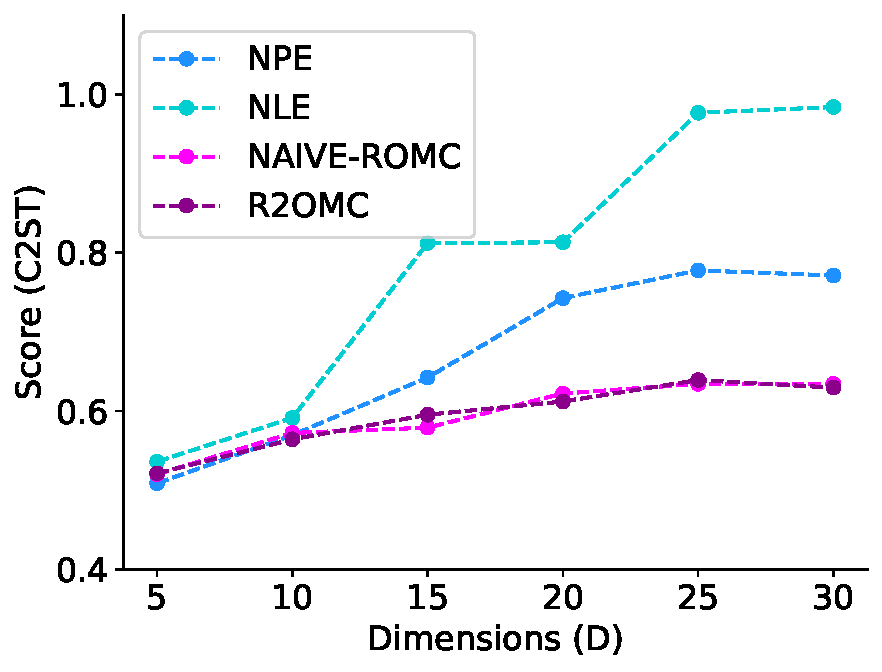
\includegraphics[width=\linewidth]{./figures/experiments/high_dim_linear_gaussian.pdf}
    \caption{$S_{\mathtt{base}}$: C2ST}
  \end{subfigure}
  \begin{subfigure}[b]{0.23\textwidth}
    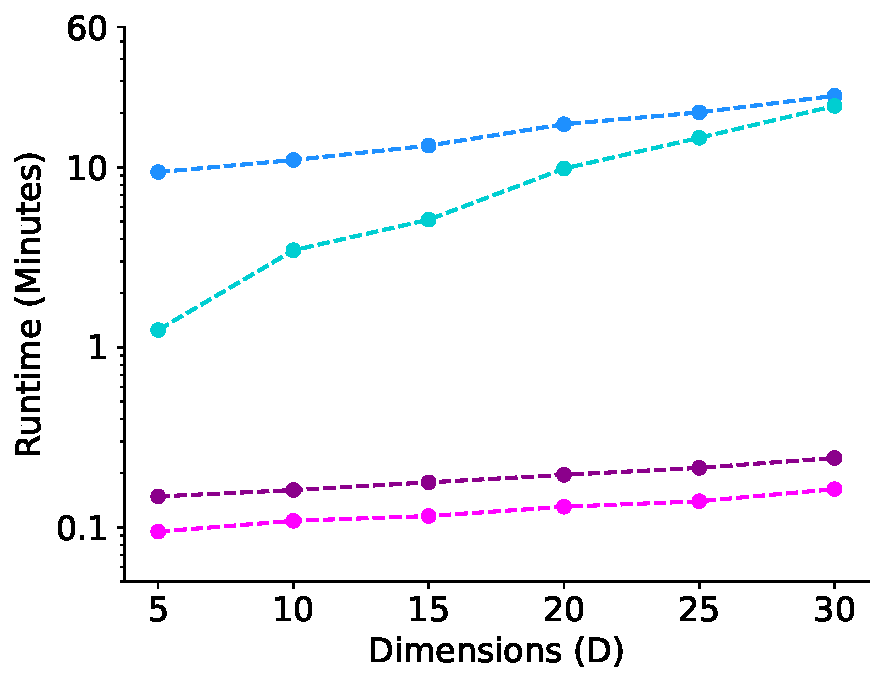
\includegraphics[width=\linewidth]{./figures/experiments/high_dim_linear_gaussian_runtimes.pdf}
    \caption{$S_{\mathtt{base}}$: Log runtime}
  \end{subfigure}\\
  \begin{subfigure}[b]{0.23\textwidth}
    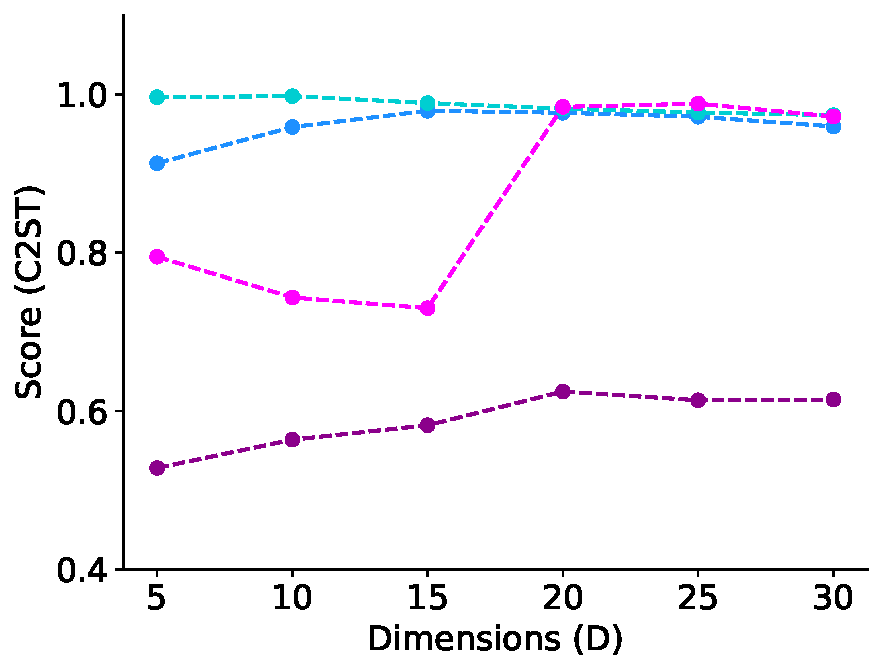
\includegraphics[width=\linewidth]{./figures/experiments/high_dim_linear_gaussian_distractors.pdf}
    \caption{$S_{\mathtt{base}}^{\mathtt{dist}}$: C2ST}
  \end{subfigure}
  \begin{subfigure}[b]{0.23\textwidth}
    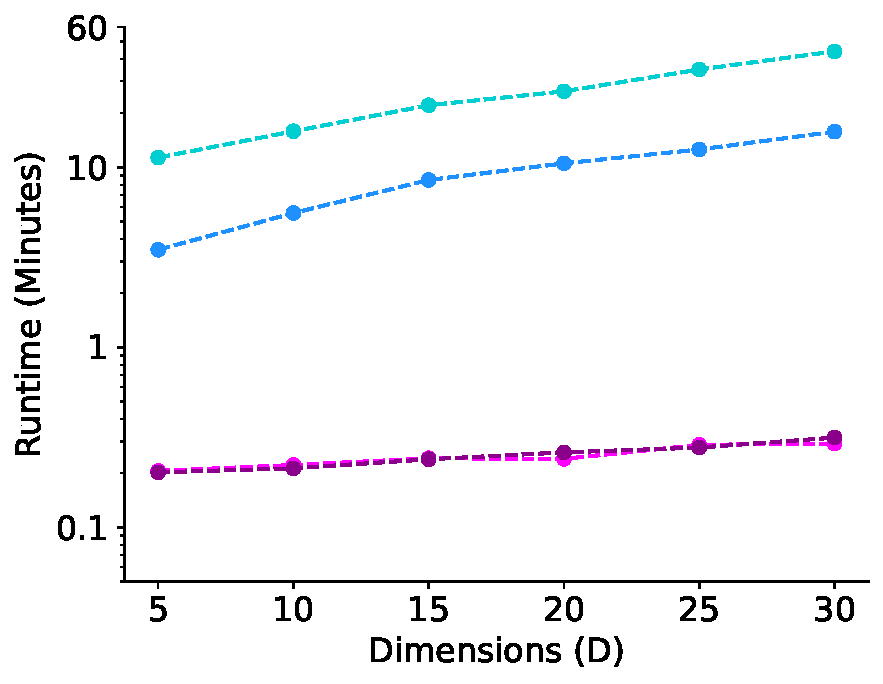
\includegraphics[width=\linewidth]{./figures/experiments/high_dim_linear_gaussian_distractors_runtimes.pdf}
    \caption{$S_{\mathtt{base}}^{\mathtt{dist}}$: Log runtime}
  \end{subfigure}
  \caption{Base simulator, varying dimensionality.}
  \label{fig:high_dim_benchmark_base}
\end{figure}

\begin{figure}[t]
  \centering
  \begin{subfigure}[b]{0.23\textwidth}
    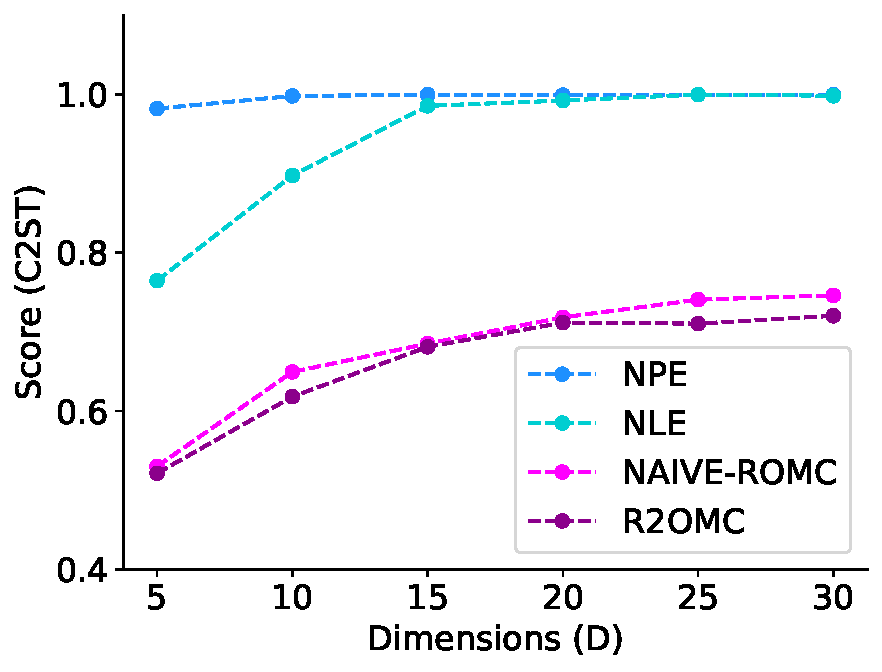
\includegraphics[width=\linewidth]{./figures/experiments/high_dim_MoG_diff_sigma.pdf}
    \caption{$S_{\mathtt{MoG}}$: C2ST}
  \end{subfigure}
  \begin{subfigure}[b]{0.23\textwidth}
    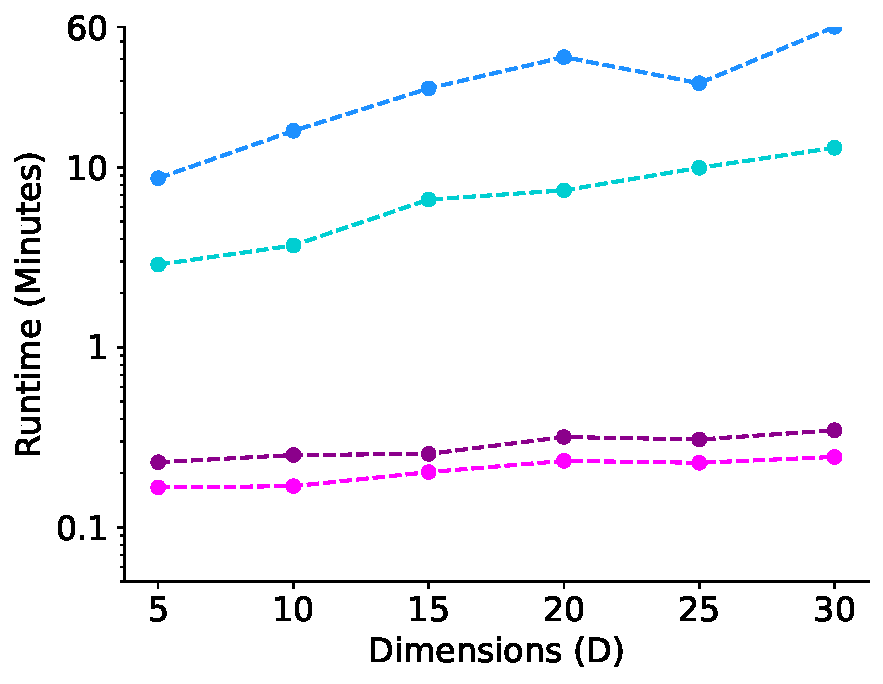
\includegraphics[width=\linewidth]{./figures/experiments/high_dim_MoG_diff_sigma_runtimes.pdf}
    \caption{$S_{\mathtt{MoG}}$: Log runtime}
  \end{subfigure}\\
  \begin{subfigure}[b]{0.23\textwidth}
    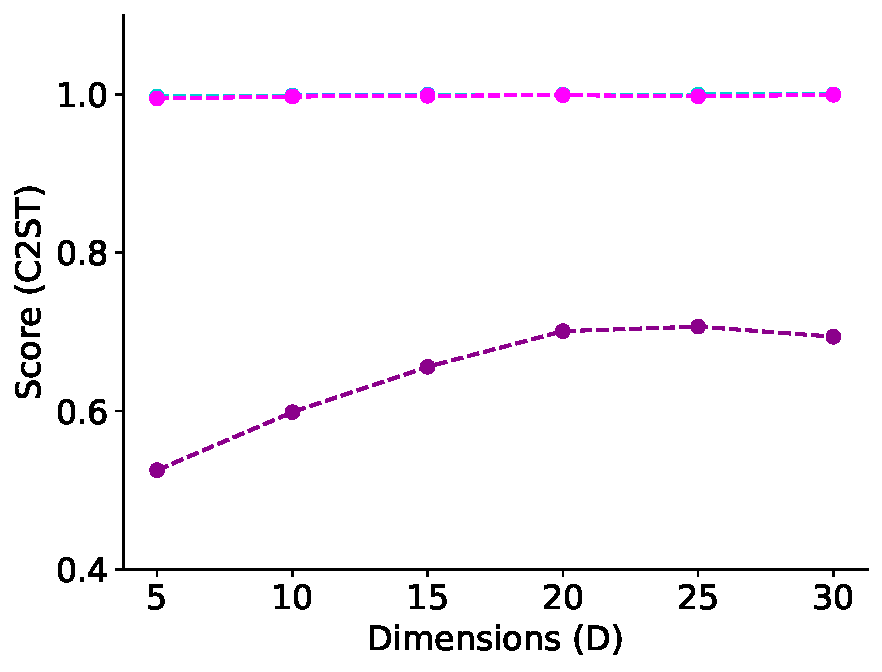
\includegraphics[width=\linewidth]{./figures/experiments/high_dim_MoG_diff_sigma_distractors.pdf}
    \caption{$S^{\mathtt{dist}}_{\mathtt{MoG}}$: C2ST}
  \end{subfigure}
  \begin{subfigure}[b]{0.23\textwidth}
    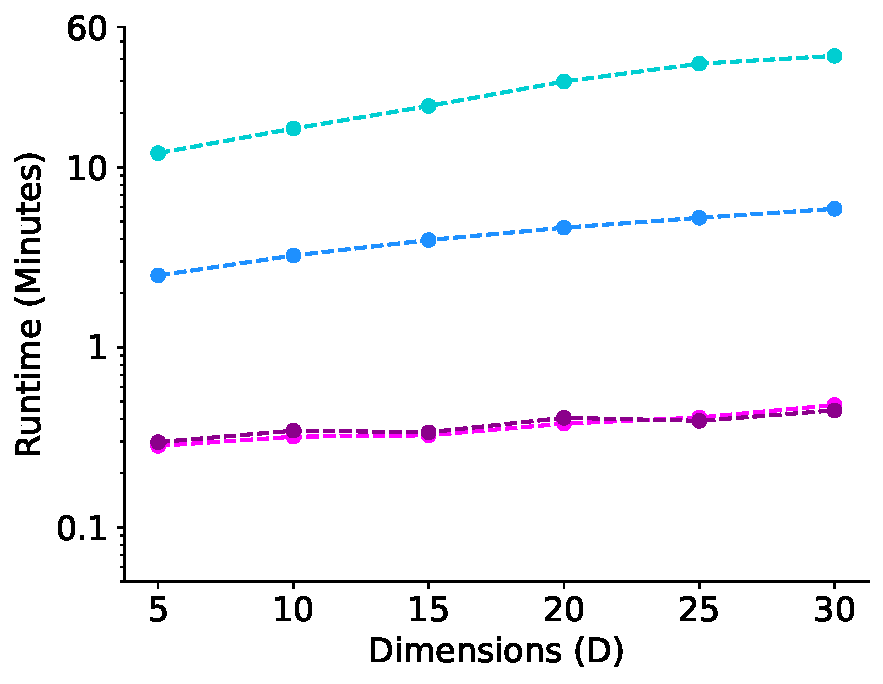
\includegraphics[width=\linewidth]{./figures/experiments/high_dim_MoG_diff_sigma_distractors_runtimes.pdf}
    \caption{$S^{\mathtt{dist}}_{\mathtt{MoG}}$: Log runtime}
  \end{subfigure}
  \caption{MoG simulator, varying dimensionality.}
  \label{fig:high_dim_benchmark_mog}
\end{figure}

We set $N=1$ and vary the dimensionality of the parameter space, using $D \in \{5, 10, 25, 30\}$. Figure~\ref{fig:high_dim_benchmark_base} shows the results for $S_{\mathtt{base}}$ with $\sigma=1.5$.
In case of no distractors, all methods perform similarly for $D<10$ in terms of accuracy but the neural methods start to struggle as $D$ increases. Both \rromc~and \nromc~ perform well as they both use gradients, enabling scalability. When distractors are added, however, all methods but \rromc~fail already at low dimensions. In terms of compute time, the ROMC-based methods are at least an order of magnitude faster. In particular note that the runtime is only weakly affected by the dimensionality. 
Figure~\ref{fig:high_dim_benchmark_mog} shows the results for $S_{\mathtt{MoG}}$ with $\sigma_1 = 0.1$ and $\sigma_2=1$. The results are largely similar except that the difference in performance is notable at low dimensions already.

% Results are presented in Figure~\ref{fig:high_dim_benchmark}.
% We observe that the increased dimensionality and the distractors pose significant challenges for \nromc and \NPE.
% In particular, \NPE~fails in all cases but the $S_{\mathtt{base}}$ simulator. In the standard version of both $S_{\mathtt{MoG}}^{\sigma_1, \sigma_2}$ simulators, and in all distractor setups, \NPE~has a \CtwoST~score close to $1.0$.
% \nromc~performs well in all standard setups, but it fails in the distractors setups for reasons described in Section \ref{sec:romc-limitations}. In contrast, \rromc~achieves a perfect \CtwoST~close to $0.5$ in all setups and dimensions
% In terms of compute time, \rromc~needs less than $10$ seconds irrespective of the setup and the dimension, while \NPE~needs more than $10$ minutes to run, even for $D=5$. Overall, the performance of \rromc in higher dimensional parameter spaces highlights the benefit of using gradient-information, both to scale to higher dimensions and to deal with distractors.

\paragraph{Multiple observations.}
\label{subsec:gaussian-multi-obs}
We set $D=10$ and vary the number $N$ of iid observations in $\{2, 5, 10, 15, 20\}$. To isolate the effect of the number of observations, we do not consider distractors. 
The results are shown in Figure~\ref{fig:multi_observation_base} for $S_{\mathtt{base}}$ ($\sigma=1$) and Figure~\ref{fig:multi_observation_mog} for $S_{\mathtt{MoG}}$ ($\sigma_1=\sigma_2=1$). 
\NPE~is strongly affected by multiple observations, breaking down quickly. \NLE~performs better but the performance deteriorates significantly as $N$ increases. While \nromc~performs well for $S_{\mathtt{base}}$, it breaks for $S_{\mathtt{MoG}}$. In contrast, \rromc~achieves good performance across all $N$. In line with the analysis in Section \ref{subsec:implementation}, the runtime increases roughly linearly with $N$ (logarithmically on the log-scale).

\begin{figure}[t] % t! puts fig 6 in the left column
    \centering
    \begin{subfigure}[b]{0.23\textwidth}
    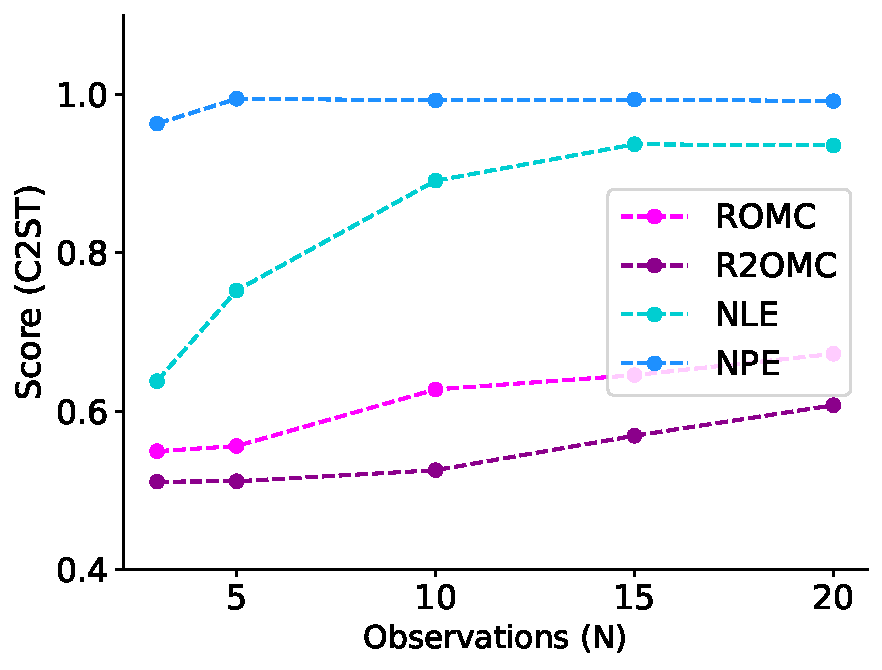
\includegraphics[width=\linewidth]{./figures/exp_multi_observation_base_c2st.pdf}
    \caption{$S_{\mathtt{base}}$: C2ST}
    \end{subfigure}
    \begin{subfigure}[b]{0.23\textwidth}
    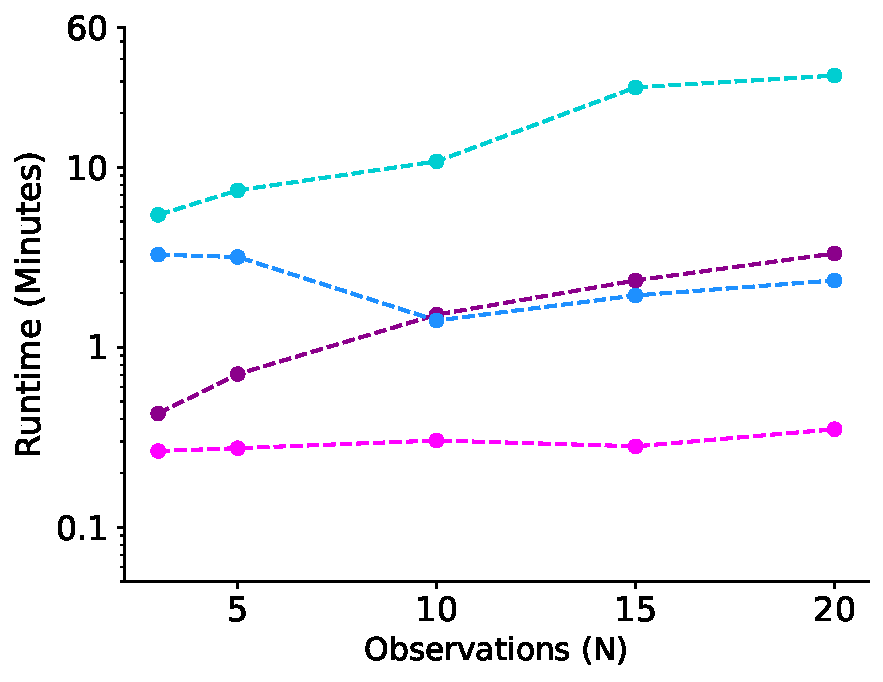
\includegraphics[width=\linewidth]{./figures/exp_multi_observation_base_runtime.pdf}
    \caption{$S_{\mathtt{base}}$: Log runtime}
  \end{subfigure}
  \caption{\label{fig:multi_observation_base} Base simulator, varying nb of observations.}
\end{figure}

\begin{figure}[t] % t! puts fig 6 in the left column
    \centering
    \begin{subfigure}[b]{0.23\textwidth}
    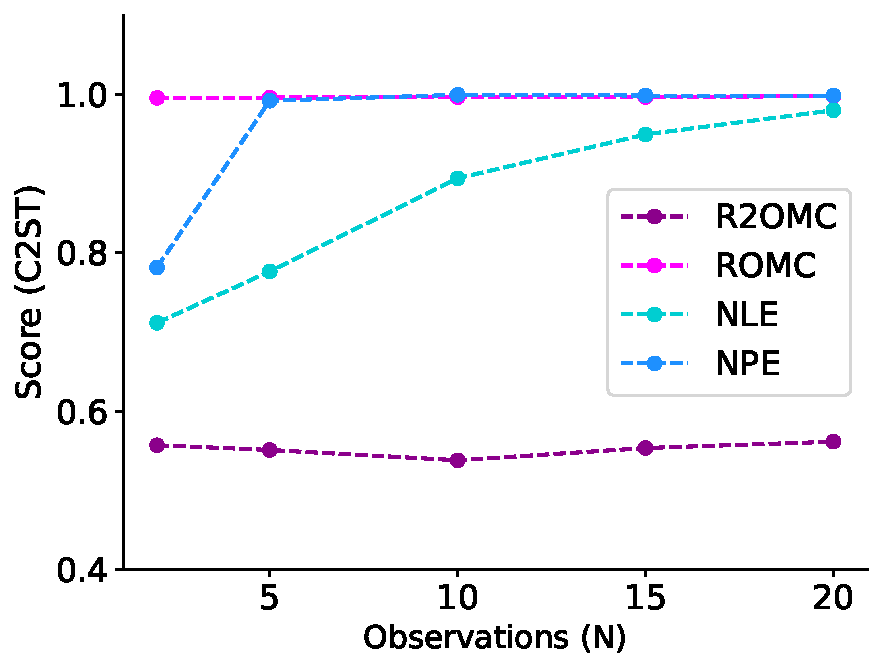
\includegraphics[width=\linewidth]{./figures/exp_multi_observation_MoG_c2st.pdf}
    \caption{$S_{\mathtt{MoG}}$: C2ST}
    \end{subfigure}
    \begin{subfigure}[b]{0.23\textwidth}
    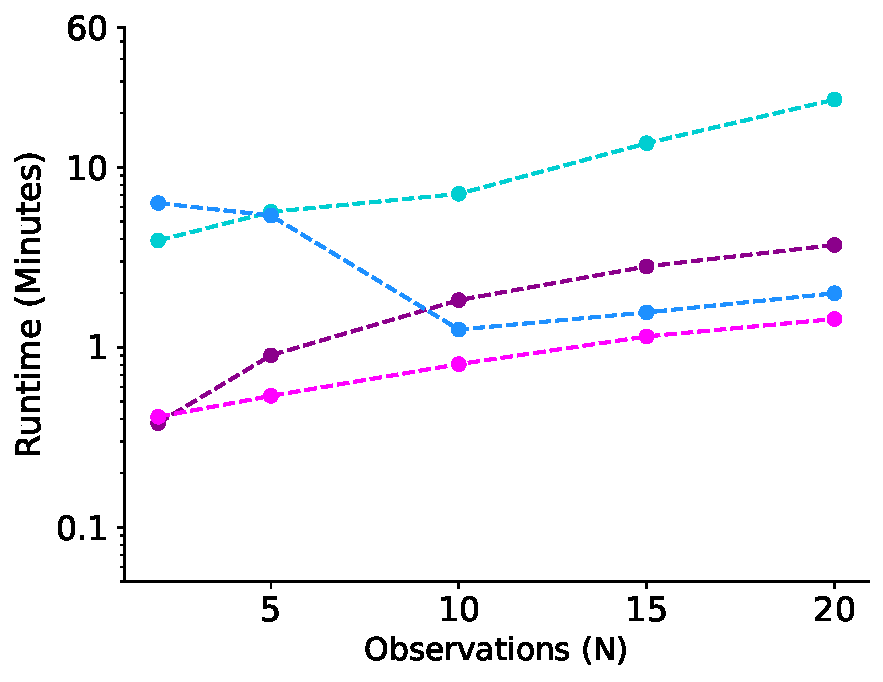
\includegraphics[width=\linewidth]{./figures/exp_multi_observation_MoG_runtime.pdf}
    \caption{$S_{\mathtt{MoG}}$: Log runtime}
    \label{subfig:high_dim_mog_diff_sigma}
  \end{subfigure}
  \caption{\label{fig:multi_observation_mog} MoG simulator, varying nb of observations.}
\end{figure}

\paragraph{Summary.}
Although the used simulators are simple, we observe that most methods struggle when the parameter dimensionality increases, multiple observations are used, or distractors (uninformative dimensions) are present, in line with Figure~\ref{fig:concept_example}. \rromc, in contrast, performs well in all-setups (\CtwoST~between 0.5 and 0.7) while running at least an order of magnitude faster than the tested neural methods.

\subsection{SBI benchmark}
\label{subsec:sbi-benchmark}

The SBI Benchmark~\citep{lueckmann2021benchmarking} enables the comparison with a range of methods. We select the following two experiments from the benchmark:
%
% \texttt{Gaussian Mixture} from the SBI Benchmark, and we add the \texttt{Linear Gaussian} experiment.
% the Gaussian Mixture, and the Linear Gaussian. The Two Moons is used to test \rromc beyond Gaussian simulators, while the Gaussian Mixture and the Linear Gaussian are used to confirm the results of the Gaussian benchmark. Furthermore, since the SBI Benchmark provides the scres of many inference methods, we can broaden the comparison of \rromc~against other methods.
% taken out for now due to space issue. Plus it's another Gaussian-based simulator, which would be too many Gaussians IMHO
% \textbf{Gaussian Linear Uniform (T.2).}
% The simulator is a 10 dimensional Gaussian $\mathcal(N)(\thb, 0.1 \mathbf{I})$ with a uniform prior $\mathcal{U}\mathbf{-1}, \mathbf{1})$ on the mean $\thb$. This creates a truncated Gaussian posterior. This is similar to the $S_{\mathtt{base}}$ simulator, but with a smaller range on the prior and fewer parameter dimensions. We include to compare to a wider range of methods.

\textbf{Gaussian Mixture (T.7).}
The simulator is $\yb|\thb \sim 0.5\mathcal{N}(\thb, \mathbf{I}) + 0.5 \mathcal{N}(\thb, 0.01 \mathbf{I})$. The parameters $\thb$ are two-dimensional and the prior is $\thb \sim \mathcal{U}(\mathbf{-10}, \mathbf{10})$. The ground truth posterior is $\thb|\data \sim 0.5 \mathcal{N}(\data, \mathbf{I}) + 0.5 \mathcal{N}(\data,0.01 \mathbf{I})$, truncated to the support of the prior. The task tests whether methods can accurately estimate a mixture of two Gaussians with same mean but one with much broader variance than the other.

\textbf{2-moons (T.8).}
The simulator is $\yb|\thb \sim  (r\cos(\alpha) + 0.25, r \sin(\alpha)) + (-|\theta_1 + \theta_2| / \sqrt{2}, (-\theta_1 + \theta_2) / \sqrt{2})$, $\alpha \sim \mathcal{U}(-\pi/2, \pi/2)$, $r \sim \mathcal{N}(0.1, 0.01^2)$.
The parameters $\thb=(\theta_1, \theta_2)$ are two-dimensional and the prior is $\thb \sim \mathcal{U}(\mathbf{-1}, \mathbf{1})$. This creates a posterior with two half-moon shape modes. %as shown in Figure~\ref{subfig:sbi_two_moons_gt}.
The task tests whether the methods can accurately estimate a posterior with both global (bimodality) and local (crescent shape) structure.

% \textbf{Linear Gaussian.}
% The simulator samples from a multivariate Gaussian with a fixed covariance; $\yb | \thb \sim \mathcal{N}(\thb, 0.1 \odot \mathbf{I})$. The parameters $\thb$ belong in $\mathbb{R}^{10}$ and the prior is $\mathcal{U}(-\mathbf{1}, \mathbf{1})$. The ground truth posterior is a unimodal Gaussian truncated by the prior, $\thb|\data = \mathcal{U}(\thb; -\mathbf{1}, \mathbf{1}) \mathcal{N}(\thb=\data, 0.1 \odot \mathbf{I})$, as shown in Figure~\ref{subfig:sbi_linear_gt}.
% The task tests whether the inference algorithms can accurately estimate a high-dimensional posterior. 


\textbf{Results.}
The results are shown in Figure~\ref{fig:sbi_experiments_two_moons}, plotting the performance in terms of \CtwoST~score versus the number of simulator runs needed. The figure shows that
\rromc~has a \CtwoST~score close to $0.5$ even with a simulation budget of $10^3$ samples, while the rest of the methods need a budget of $10^5$ or more to achieve a similar score and perform much worse for smaller budgets. As in the Gaussian benchmark, we observe that most SBI methods fail to produce accurate posterior samples without a large simulation budget even in relatively simple tasks.

\begin{figure}
  \centering
  % taken out due to space issues. Plus, it's another Gaussian, which would make the simulations too Gaussian heavy.
  % \begin{subfigure}[b]{.24\linewidth}
  %   \centering
  %   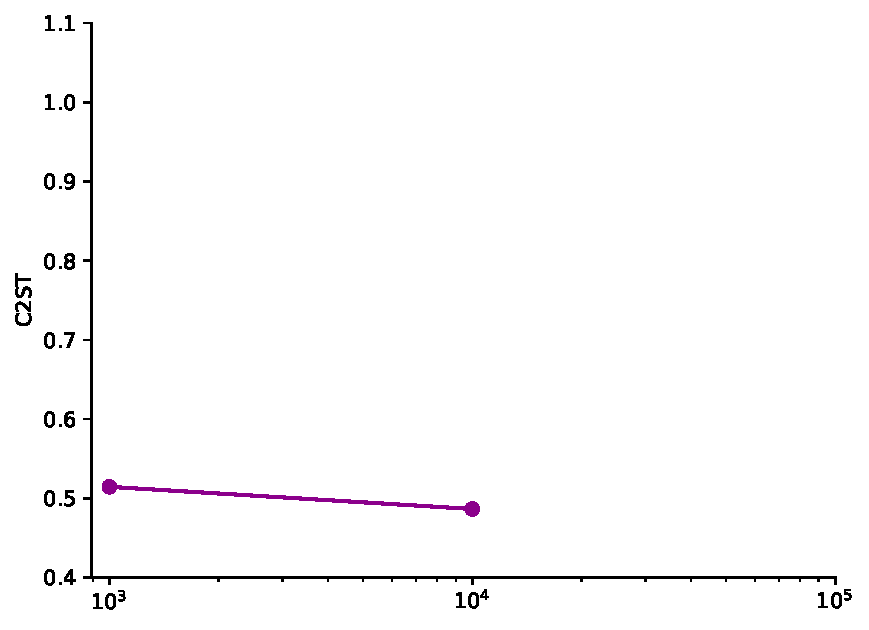
\includegraphics[width=\linewidth]{./figures/two_moons_romc.pdf}
  %   \caption{\texttt{R2OMC (C2ST)}}
  %   \label{subfig:sbi_two_moons_r2omc}
  % \end{subfigure}\\
  % \begin{subfigure}[b]{\linewidth}
  %   \centering
  %   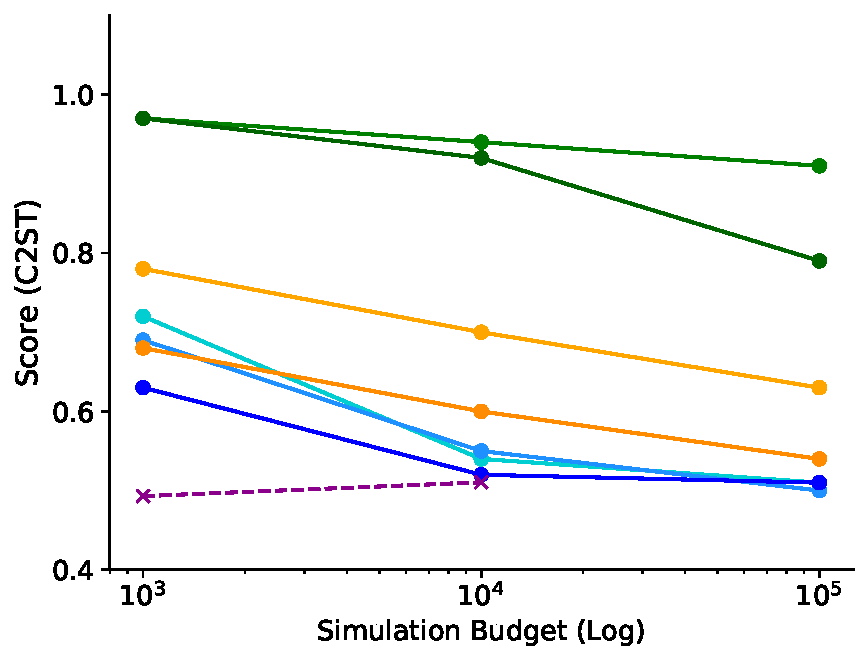
\includegraphics[width=0.6\linewidth]{./figures/gaussian_linear_uniform.pdf}
  %   \caption{Gaussian Linear Uniform}
  %   \label{subfig:sbi_gaussian_mixture_r2omc}
  % \end{subfigure}
  \begin{subfigure}[b]{0.49\linewidth}
     \centering
     \includegraphics[width=\linewidth]{./figures/gaussian_mixture.pdf}
     \caption{Mixture of Gaussians}
     \label{subfig:sbi_gaussian_mixture_r2omc}
   \end{subfigure}
  \begin{subfigure}[b]{.49\linewidth}
    \centering
    \includegraphics[width=\linewidth]{./figures/two_moons.pdf}
    \caption{2-moons}
    \label{subfig:sbi_two_moons_rest}
  \end{subfigure}
  \caption{SBI benchmark: performance (C2ST) vs compute budget (log number of simulator runs).}
  \label{fig:sbi_experiments_two_moons}
\end{figure}

\subsection{Image Example}

\begin{figure*}
  \centering
  \setlength{\tabcolsep}{1pt}
  \renewcommand{\arraystretch}{2}
  \begin{tabular}{*{10}{c} >{\centering\arraybackslash}m{0.1\textwidth}}
    \imagerow{image_pixelwise}{image_clean}{Clean: $\thb^*$}
    \hline
    \imagerow{image_pixelwise}{image_observation}{Observed: $\data$}
    \imagerow{image_pixelwise}{posterior_mean}{Posterior mean}
    \imagerow{image_pixelwise}{posterior_std}{Posterior std}
    \hline
    \imagerow{image_checkerboard}{image_observation}{Observed: $\data$}
    \imagerow{image_checkerboard}{posterior_mean}{Posterior mean}
    \imagerow{image_checkerboard}{posterior_std}{Posterior std}
  \end{tabular}
  \caption{Your figure caption here.}
  \label{fig:pixelwise}
\end{figure*}

\section{Conclusion}
\label{sec:conclusion}

We have presented \rromc, a new Bayesian inference method for simulator models that addresses three key scalability challenges in simulation-based (likelihood-free) inference, namely high-dimensional parameter spaces, multiple observations, and the possible presence of uninformative dimensions (i.e., distractors). R2OMC builds on the ROMC framework and formulates the inference problem in terms of a set of deterministic optimization problems that can be solved with gradient-descent, enabling inference in high-dimensional parameter spaces. It further introduces a gradient-based filtering step to mask distractors during inference. It uses a novel adaptive importance sampling approach that efficiently identifies posterior samples that explain \emph{all} available iid observations. We offer an efficient \texttt{JAX}-based implementation that leverages key auto-differentiation and vectorization features to accelerate the inference. Simulations performed with novel experimental settings as well as the comprehensive SBI benchmark show that R2OMC achieves improved accuracy (close to the optimal $0.5$ \texttt{C2ST}) compared to existing methods, while using a smaller number of simulator calls and a fraction of the computational time. 


% The results are very promising; even without any methodological improvements, ROMC seems to perform much beyond the state-of-the-art most problems. I discuss below the limitations we can focus on.

% \subsection{Multiple Observations}

% When dealing with multiple observations (as in the SLCP problem) $\data = [\data_1, \cdots, \data_N]$, the OMC scheme doesn't perform well. This is because we are not optimizing over unobserved (latent) variables.

% For example, suppose we have a latent variable $k$ drawn from a Bernoulli distribution, $k \sim \mathcal{B}(0.5)$. When $k=0$, the observation is then sampled from $\mathcal{N}(-\thb, \mathbf{I})$, and when $k=1$, it's sampled from $\mathcal{N}(\thb, \mathbf{I})$. Let's say we have two observations $\data_1 = (5.1, 4.9)$ and $\data_2 = (-5, -5.1)$. The ground truth posterior has two gaussian modes with centers around $\pm (5, 5)$.

% However, if we apply OMC as is, meaning optimizing over a flat vector of observations $\data = (5.1, 4.9, -5, -5.1)$, it will give a Gaussian with a center at $(0,0)$ and high covariance.

% \paragraph{Ideas.}

% Optimize independently for each observation, meaning for $\mathtt{seed}[i]$, optimize separately for $\data_1$ and $\data_2$, and accept two bounding boxes, one for each observation.
% Does this approach makes sense? If so, could we show it theoretically as well?

% \subsection{Epsilon thresholds}

% ROMC works with three acceptance thresholds: \(\epsilon_1\) for accepting \(\thb_*\), \(\epsilon_2\) for the proposal area, and \(\epsilon_3\) for accepting samples. Setting these thresholds is not straightforward; in problems with distractors, the distance to the observation is heavily influenced by them. As a result, certain seeds have much smaller distances than others, leading to larger proposal areas and dominating the posterior, regardless of the \(\epsilon_2\) threshold.

% \paragraph{Ideas.}


% \subsection{Hybrid Schema}

% ROMC is only capable of sampling from the posterior distribution. It would be intresting to propose a solution that not only samples from the posterior but also models it, meaning it provides a $\mathtt{.log\_prob()}$ method in addition to $\mathtt{.sample()}$.

% \paragraph{Ideas.}
% The initial idea was to utilize ROMC as the first step in supplying training samples for neural-based SBI methods. This approach would render the hybrid method $\epsilon$-free, addressing some of the discussed issues. The concept relies on the observation that NRE, NPE, and NLE perform significantly better in their sequential versions, where the proposal area is updated sequentially to mimic the posterior distribution. \textbf{However, I encountered difficulties in making this approach effective; I attempted to train NPE using the samples provided by ROMC but didn't observe significant improvement, except in the case of the linear Gaussian example.}

% Interestingly, simply fitting a Mixture of Gaussians (MoG) yielded much better results. However, MoG has the limitation that the user needs to manually determine the number of components, which is challenging without intuition about the posterior's shape. In the current experiments, setting it to 50 seems to work well.

% \subsection{More experiments.}

% I want to test ROMC in more problems.

% \paragraph{Ideas.}

% The SLCP example will demonstrate how the method performs with multiple observations when the posterior is multi-modal and asymmetric.
% A series of problems involving distractors will examine whether the method can identify uninformative dimensions of the observation.
% Regarding real-case problems, the SBI Benchmark includes SIR and Lotka-Volterra, but I'm unsure if the simulator is differentiable in these cases. If not, we need to find additional examples.

\clearpage

\bibliographystyle{unsrtnat}
\bibliography{paper}
% \section{GENERAL FORMATTING INSTRUCTIONS}

% Submissions are limited to \textbf{8 pages} excluding references. 
% There will be an additional page for camera-ready versions of the accepted papers.

% Papers are in 2 columns with the overall line width of 6.75~inches (41~picas).
% Each column is 3.25~inches wide (19.5~picas).  The space
% between the columns is .25~inches wide (1.5~picas).  The left margin is 0.88~inches (5.28~picas).
% Use 10~point type with a vertical spacing of
% 11~points. Please use US Letter size paper instead of A4.

% Paper title is 16~point, caps/lc, bold, centered between 2~horizontal rules.
% Top rule is 4~points thick and bottom rule is 1~point thick.
% Allow 1/4~inch space above and below title to rules.

% Author descriptions are center-justified, initial caps.  The lead
% author is to be listed first (left-most), and the Co-authors are set
% to follow.  If up to three authors, use a single row of author
% descriptions, each one center-justified, and all set side by side;
% with more authors or unusually long names or institutions, use more
% rows.

% Use one-half line space between paragraphs, with no indent.

% \section{FIRST LEVEL HEADINGS}

% First level headings are all caps, flush left, bold, and in point size
% 12. Use one line space before the first level heading and one-half line space
% after the first level heading.

% \subsection{Second Level Heading}

% Second level headings are initial caps, flush left, bold, and in point
% size 10. Use one line space before the second level heading and one-half line
% space after the second level heading.

% \subsubsection{Third Level Heading}

% Third level headings are flush left, initial caps, bold, and in point
% size 10. Use one line space before the third level heading and one-half line
% space after the third level heading.

% \paragraph{Fourth Level Heading}

% Fourth level headings must be flush left, initial caps, bold, and
% Roman type.  Use one line space before the fourth level heading, and
% place the section text immediately after the heading with no line
% break, but an 11 point horizontal space.

% %%%
% \subsection{Citations, Figure, References}


% \subsubsection{Citations in Text}

% Citations within the text should include the author's last name and
% year, e.g., (Cheesman, 1985). 
% %Apart from including the author's last name and year, citations can follow any style, as long as the style is consistent throughout the paper.  
% Be sure that the sentence reads
% correctly if the citation is deleted: e.g., instead of ``As described
% by (Cheesman, 1985), we first frobulate the widgets,'' write ``As
% described by Cheesman (1985), we first frobulate the widgets.''


% The references listed at the end of the paper can follow any style as long as it is used consistently.

% %Be sure to avoid
% %accidentally disclosing author identities through citations.

% \subsubsection{Footnotes}

% Indicate footnotes with a number\footnote{Sample of the first
%   footnote.} in the text. Use 8 point type for footnotes. Place the
% footnotes at the bottom of the column in which their markers appear,
% continuing to the next column if required. Precede the footnote
% section of a column with a 0.5 point horizontal rule 1~inch (6~picas)
% long.\footnote{Sample of the second footnote.}

% \subsubsection{Figures}

% All artwork must be centered, neat, clean, and legible.  All lines
% should be very dark for purposes of reproduction, and art work should
% not be hand-drawn.  Figures may appear at the top of a column, at the
% top of a page spanning multiple columns, inline within a column, or
% with text wrapped around them, but the figure number and caption
% always appear immediately below the figure.  Leave 2 line spaces
% between the figure and the caption. The figure caption is initial caps
% and each figure should be numbered consecutively.

% Make sure that the figure caption does not get separated from the
% figure. Leave extra white space at the bottom of the page rather than
% splitting the figure and figure caption.
% \begin{figure}[h]
% \vspace{.3in}
% \centerline{\fbox{This figure intentionally left non-blank}}
% \vspace{.3in}
% \caption{Sample Figure Caption}
% \end{figure}

% \subsubsection{Tables}

% All tables must be centered, neat, clean, and legible. Do not use hand-drawn tables.
% Table number and title always appear above the table.
% See Table~\ref{sample-table}.

% Use one line space before the table title, one line space after the table title,
% and one line space after the table. The table title must be
% initial caps and each table numbered consecutively.

% \begin{table}[h]
% \caption{Sample Table Title} \label{sample-table}
% \begin{center}
% \begin{tabular}{ll}
% \textbf{PART}  &\textbf{DESCRIPTION} \\
% \hline \\
% Dendrite         &Input terminal \\
% Axon             &Output terminal \\
% Soma             &Cell body (contains cell nucleus) \\
% \end{tabular}
% \end{center}
% \end{table}

% \section{SUPPLEMENTARY MATERIAL}

% If you need to include additional appendices during submission, you can include them in the supplementary material file.
% You can submit a single file of additional supplementary material which may be either a pdf file (such as proof details) or a zip file for other formats/more files (such as code or videos). 
% Note that reviewers are under no obligation to examine your supplementary material. 
% If you have only one supplementary pdf file, please upload it as is; otherwise gather everything to the single zip file.

% You must use \texttt{aistats2025.sty} as a style file for your supplementary pdf file and follow the same formatting instructions as in the main paper. 
% The only difference is that it must be in a \emph{single-column} format.
% You can use \texttt{supplement.tex} in our starter pack as a starting point.
% Alternatively, you may append the supplementary content to the main paper and split the final PDF into two separate files.

% \section{SUBMISSION INSTRUCTIONS}

% To submit your paper to AISTATS 2025, please follow these instructions.

% \begin{enumerate}
%     \item Download \texttt{aistats2025.sty}, \texttt{fancyhdr.sty}, and \texttt{sample\_paper.tex} provided in our starter pack. 
%     Please, do not modify the style files as this might result in a formatting violation.
    
%     \item Use \texttt{sample\_paper.tex} as a starting point.
%     \item Begin your document with
%     \begin{flushleft}
%     \texttt{\textbackslash documentclass[twoside]\{article\}}\\
%     \texttt{\textbackslash usepackage\{aistats2025\}}
%     \end{flushleft}
%     The \texttt{twoside} option for the class article allows the
%     package \texttt{fancyhdr.sty} to include headings for even and odd
%     numbered pages.
%     \item When you are ready to submit the manuscript, compile the latex file to obtain the pdf file.
%     \item Check that the content of your submission, \emph{excluding} references and reproducibility checklist, is limited to \textbf{8 pages}. The number of pages containing references and reproducibility checklist only is not limited.
%     \item Upload the PDF file along with other supplementary material files to the CMT website.
% \end{enumerate}

% \subsection{Camera-ready Papers}

% %For the camera-ready paper, if you are using \LaTeX, please make sure
% %that you follow these instructions.  
% % (If you are not using \LaTeX,
% %please make sure to achieve the same effect using your chosen
% %typesetting package.)

% If your papers are accepted, you will need to submit the camera-ready version. Please make sure that you follow these instructions:
% \begin{enumerate}
%     %\item Download \texttt{fancyhdr.sty} -- the
%     %\texttt{aistats2022.sty} file will make use of it.
%     \item Change the beginning of your document to
%     \begin{flushleft}
%     \texttt{\textbackslash documentclass[twoside]\{article\}}\\
%     \texttt{\textbackslash usepackage[accepted]\{aistats2025\}}
%     \end{flushleft}
%     The option \texttt{accepted} for the package
%     \texttt{aistats2025.sty} will write a copyright notice at the end of
%     the first column of the first page. This option will also print
%     headings for the paper.  For the \emph{even} pages, the title of
%     the paper will be used as heading and for \emph{odd} pages the
%     author names will be used as heading.  If the title of the paper
%     is too long or the number of authors is too large, the style will
%     print a warning message as heading. If this happens additional
%     commands can be used to place as headings shorter versions of the
%     title and the author names. This is explained in the next point.
%     \item  If you get warning messages as described above, then
%     immediately after $\texttt{\textbackslash
%     begin\{document\}}$, write
%     \begin{flushleft}
%     \texttt{\textbackslash runningtitle\{Provide here an alternative
%     shorter version of the title of your paper\}}\\
%     \texttt{\textbackslash runningauthor\{Provide here the surnames of
%     the authors of your paper, all separated by commas\}}
%     \end{flushleft}
%     Note that the text that appears as argument in \texttt{\textbackslash
%       runningtitle} will be printed as a heading in the \emph{even}
%     pages. The text that appears as argument in \texttt{\textbackslash
%       runningauthor} will be printed as a heading in the \emph{odd}
%     pages.  If even the author surnames do not fit, it is acceptable
%     to give a subset of author names followed by ``et al.''

%     %\item Use the file sample\_paper.tex as an example.

%     \item The camera-ready versions of the accepted papers are \textbf{9
%       pages}, plus any additional pages needed for references and reproducibility checklist.

%     \item If you need to include additional appendices,
%       you can include them in the supplementary
%       material file.

%     \item Please, do not change the layout given by the above
%       instructions and by the style file.

% \end{enumerate}

% \subsubsection*{Acknowledgements}
% All acknowledgments go at the end of the paper, including thanks to reviewers who gave useful comments, to colleagues who contributed to the ideas, and to funding agencies and corporate sponsors that provided financial support. 
% To preserve the anonymity, please include acknowledgments \emph{only} in the camera-ready papers.


% \subsubsection*{References}

% References follow the acknowledgements.  Use an unnumbered third level
% heading for the references section.  Please use the same font
% size for references as for the body of the paper---remember that
% references do not count against your page length total.

% % \begin{thebibliography}{}
% % \setlength{\itemindent}{-\leftmargin}
% % \makeatletter\renewcommand{\@biblabel}[1]{}\makeatother
% % \bibitem{} J.~Alspector, B.~Gupta, and R.~B.~Allen (1989).
% %     \newblock Performance of a stochastic learning microchip.
% %     \newblock In D. S. Touretzky (ed.),
% %     \textit{Advances in Neural Information Processing Systems 1}, 748--760.
% %     San Mateo, Calif.: Morgan Kaufmann.

% % \bibitem{} F.~Rosenblatt (1962).
% %     \newblock \textit{Principles of Neurodynamics.}
% %     \newblock Washington, D.C.: Spartan Books.

% % \bibitem{} G.~Tesauro (1989).
% %     \newblock Neurogammon wins computer Olympiad.
% %     \newblock \textit{Neural Computation} \textbf{1}(3):321--323.
% % \end{thebibliography}



%%%%%%%%%%%%%%%%%%%%%%%%%%%%%%%%%%%%%%%%%%%%%%%%%%%%%%%%%%%%
\section*{Checklist}


% %%% BEGIN INSTRUCTIONS %%%
The checklist follows the references. For each question, choose your answer from the three possible options: Yes, No, Not Applicable.  You are encouraged to include a justification to your answer, either by referencing the appropriate section of your paper or providing a brief inline description (1-2 sentences). 
Please do not modify the questions.  Note that the Checklist section does not count towards the page limit. Not including the checklist in the first submission won't result in desk rejection, although in such case we will ask you to upload it during the author response period and include it in camera ready (if accepted).

\textbf{In your paper, please delete this instructions block and only keep the Checklist section heading above along with the questions/answers below.}
% %%% END INSTRUCTIONS %%%


 \begin{enumerate}


 \item For all models and algorithms presented, check if you include:
 \begin{enumerate}
   \item A clear description of the mathematical setting, assumptions, algorithm, and/or model. [Yes]
   \item An analysis of the properties and complexity (time, space, sample size) of any algorithm. [Yes]
   \item (Optional) Anonymized source code, with specification of all dependencies, including external libraries. [No]
 \end{enumerate}


 \item For any theoretical claim, check if you include:
 \begin{enumerate}
   \item Statements of the full set of assumptions of all theoretical results. [Not Applicable]
   \item Complete proofs of all theoretical results. [Not Applicable]
   \item Clear explanations of any assumptions. [Not Applicable]   
 \end{enumerate}


 \item For all figures and tables that present empirical results, check if you include:
 \begin{enumerate}
   \item The code, data, and instructions needed to reproduce the main experimental results (either in the supplemental material or as a URL). [No] Not now, but code will be made available if accepted.
   \item All the training details (e.g., data splits, hyperparameters, how they were chosen). [Yes]
         \item A clear definition of the specific measure or statistics and error bars (e.g., with respect to the random seed after running experiments multiple times). [Yes]
         \item A description of the computing infrastructure used. (e.g., type of GPUs, internal cluster, or cloud provider). [Yes]
 \end{enumerate}

 \item If you are using existing assets (e.g., code, data, models) or curating/releasing new assets, check if you include:
 \begin{enumerate}
   \item Citations of the creator If your work uses existing assets. [Yes]
   \item The license information of the assets, if applicable. [Yes]
   \item New assets either in the supplemental material or as a URL, if applicable. [Not Applicable]
   \item Information about consent from data providers/curators. [Not Applicable]
   \item Discussion of sensible content if applicable, e.g., personally identifiable information or offensive content. [Not Applicable]
 \end{enumerate}

 \item If you used crowdsourcing or conducted research with human subjects, check if you include:
 \begin{enumerate}
   \item The full text of instructions given to participants and screenshots. [Not Applicable]
   \item Descriptions of potential participant risks, with links to Institutional Review Board (IRB) approvals if applicable. [Not Applicable]
   \item The estimated hourly wage paid to participants and the total amount spent on participant compensation. [Not Applicable]
 \end{enumerate}

 \end{enumerate}


\clearpage
\appendix
\onecolumn
\if0
\section{Catalog of Symbols}
\label{app-sec:symbols}

\begin{table}[!ht]
  \centering
  \begin{tabular}{ll}
    \toprule
    Symbol & Description \\
    \midrule
    $\thb \in \mathbb{R}^D$ & Parameters \\
    $\ub$ & Nuisance variables \\
    $\yb \in \mathbb{R}^{D_{\yb}}$ & Simulator output \\
    $\data \in \mathbb{R}^{D_{\yb}}$ & Observation (if single) \\
    $\data_n$ & $n$-th observation (if multiple) \\
    $ \{ \data_n \}_{n=1}^N$ & Set of observations \\
    $\jac_{\thb}$ & Jacobian of the simulator at $\thb$ \\
    \midrule
    $p(\thb)$ & Prior distribution of the parameters \\
    $p(\ub)$ & Prior distribution of the nuisance variables \\
    $L_{\epsilon}(\thb)$ & ABC likelihood \\
    $L_{\epsilon}^n(\thb, \ub)$ & ABC likelihood for the $n$-th observation \\
    $p_{\epsilon}(\thb | \data)$ & ABC posterior (single observation) \\
    $p_{\epsilon}(\thb | \{ \data_n \}_{n=1}^N)$ & ABC posterior (multiple observations) \\
    $q(\thb)$ & Proposal distribution \\
    $q_i(\thb)$ & Proposal distribution for the $i$-th seed \\
    \midrule
    $g(\thb, \ub)$ & Simulator \\
    $d(\thb) = d(g(\thb, \ub), \data)$ & Distance function \\
    $d_i(\thb) = d(g(\thb, \ub_i), \data)$ & Distance function for the $i$-th seed \\
    \midrule
    $\accregioni$ & Acceptance region for the $i$-th seed \\
    % $d(\thb, \data)$ & Distance function \\
    % $d_i(\thb)$ & Distance function for the $i$-th seed \\
    % $\thb_i^*$ & Optimal point for the $i$-th seed \\
    % $\jac$ & Jacobian of the simulator \\
    % $w_i$ & Weight of the $i$-th seed \\
    % $q_i$ & Proposal distribution for the $i$-th seed \\
    % $V_i$ & Proposal area for the $i$-th seed \\
    % $\epsilon$ & Acceptance threshold for the optimal point \\
    % $\epsilon_2$ & Acceptance threshold for the proposal area \\
    % $\epsilon_3$ & Acceptance threshold for the samples \\
    \midrule
    $S$ & Number of seeds \\
    $M$ & Number of samples per proposal area \\
    $N$ & Number of observations \\
    $P$ & Number of samples at \rromc, Eq. (\ref{eq:romc_weight}) \\
    \midrule
    $n = 1, \ldots, N$ & Index of the observation \\
    $i = 1, \ldots, S$ & Index of the seed \\
    $j = 1, \ldots, M$ & Index of the sample \\
    \bottomrule
  \end{tabular}
  \caption{Catalog of symbols used in the paper.}
  \label{tab:symbols}
\end{table}
\fi

\section{Methods}
\label{app-sec:methods}

Throughout the paper we run experiments based on four methods: R2OMC (our proposal), NAIVE-ROMC~\citep[a straightforward use of the ROMC framework by][]{ikonomov2020robust}, Neural Posterior Estimation (NPE)~\citep{greenberg2019automatic}, Neural Likelihood Estimation (NLE)~\citep{papamakarios2019sequential}.

\paragraph{R2OMC.}

A detailed description of the method can be found in Algorithm~\ref{alg:r2omc}. 

In Step 2 of Algorithm~\ref{alg:r2omc}, i.e., computing the uninformative dimensions, we typically use around 50 samples from the distribution \(p(u)\) and another 50 samples from \(p(\thb)\), with the parameter \(\tau\) set to machine precision, i.e., \(\tau \approx 0\). Similar results can be obtained with fewer samples, such as 10 or 20.

For Step 3, i.e., computing the optimal points \(\thb_{i,n}^*\), we use the Adam optimizer, with a learning rate between 0.01 and 0.2, depending on the specific problem. Our default choice is 0.1. The number of optimization steps varies between 100 and 400, with 50 as the  default. The distance function \(d(\thb)\) is defined as the squared Euclidean distance between the simulator output and the observation, i.e., \(d(\thb) = \|\yb - \data_n\|^2_2\).
The number of seeds \(S\) used ranges from 500 to 5000, with 1000 as the default. The number of seeds corresponds to the simulation budget; for example, if a budget of 10,000 runs is available, we use (at most) 10,000 seeds. Typically, we select 80\% of the seeds based on the best \(d_i^n(\thb_{i,n}^*)\). However, the percentage of accepted seeds can vary between 50\% and 100\%, depending on the absolute values of \(d_i^n(\thb_{i,n}^*)\) for \(i = 1, \dots, S\).

For Step 5, i.e., constructing the hyperboxes, we use Algorithm~\ref{alg:region_construction}. We normally set \(\epsilon\) to be twice the distance of the `worst' accepted seed, i.e., \(\epsilon = 2 \max_i d_i^n(\thb_{i,n}^*)\), where \(i\) is an index over the accepted seeds. Alternatively, \(\epsilon\) can be set to a fixed value such as $0.1$. The typical settings for step size, number of steps, and refinements are \(\eta = 0.1\), \(L = 100\), and \(R = 1\), respectively.

For Step 7, i.e., sampling from the proposal distribution, we generate between 1000 and 100,000 candidate samples, with the default being 5000. From these candidates, we select 1000 via weighted sampling.
For computing the weights, $\{w_p\}_{p=1}^{P}$, we set $\epsilon$ to a value about twice the distance of the `worst' accepted seed, i.e., $\epsilon = 2 \max_{i,n} d_i^n(\thb_{i,n}^*)$. However, this can vary depending on the problem, and by testing different values.

Finally, we keep 1000 posterior samples, which are used to compute the \texttt{C2ST} score using another 1000 samples drawn from the true posterior.

\begin{algorithm}[!ht]
  \caption{Hyperbox Computation \newline
    \textit{Input:} Optimal point \(\thb^*\), distance function \(d(\thb)\), Jacobian \(\jac\) at \(\thb^*\) \newline
    \textit{Parameters:} Step size \(\eta\), number of refinements \(R\), number of steps \(L\), distance threshold \(\epsilon\)}
  \label{alg:region_construction}
  \begin{algorithmic}[1]
    \State Compute eigenvectors \(\vb_d\) of \(\jac^T\jac\) {\scriptsize (\(d = 1,\ldots,D)\)}
    \For{\(d = 1\) to \(D\)}
      \State Initialize endpoint \(\Tilde{\thb} \gets \thb^*\)
      \State Set refinement counter \(r \gets 0\)
      \Repeat{}
        \State Set step counter \(l \gets 0\)
        \Repeat{}
          \State Increment step counter \(l \gets l + 1\)
          \State Update \(\Tilde{\thb} \gets \Tilde{\thb} + \eta \vb_d\)
        \Until{\(d(\thb) > \epsilon\) or \(l = L\)}
        \State Move back one step \(\Tilde{\thb} \gets \Tilde{\thb} - \eta \vb_d\)
        \State Halve the step size \(\eta \gets \eta/2\)
        \State Increment refinement counter \(r \gets r + 1\)
      \Until{\(r = R\)}
      \State Set \(\Tilde{\thb}\) as the endpoint
      \State Repeat steps 3-15 for \(\vb_d = - \vb_d\) and set \(\Tilde{\thb}\) as the negative endpoint
    \EndFor
    \State Define a uniform distribution \(q\) over the hyperbox
    \State \Return \(q\)
  \end{algorithmic}
\end{algorithm}


\paragraph{NAIVE-ROMC.}

We use the Algorithm presented as ROMC in~\cite{ikonomov2020robust}. The characterization NAIVE indicates the use of a naive distance function in case of multiple observations. As described in the main paper, in case of $N$ observations, we concatenate them in a single vector $\data = (\mathbf{y}^{o, (1)}, \ldots, \mathbf{y}^{o, (N)})$, then, run the simulator $N$ times, concatenate the ouputs, $\yb = (\yb^{(1)}, \ldots, \yb^{(N)})$ and set the distance to be the squared Euclidean distance between the two vectors, $d(\thb) = ||\yb-\data||_2^2$.
Although using this approach for defining $d(\thb)$ has disadvantages, that is why we name it `NAIVE', there is no other (simple) approach that leads to a better posterior approximation, under multiple observations.

\nromc~is practically the same as \rromc~(Algorithm~\ref{alg:r2omc} of the main text), if (a) we omit Step 2, i.e., computing the uninformative dimensions and (b) set $N=1$.
This is why \nromc~and \rromc~have a similar \texttt{C2ST} score in problems without distractors and with a single observation.
In case of multiple observations, we use as $\yb$ and $\data$, the concatenated vectors as described above.
For \nromc, we use a $\texttt{JAX}$-based implementation that is similar to the one we use for \rromc. The reason for not using its existing implementation~\citep{gkolemis2023extendable} of the ELFI package~\citep{elfipackage} is that it does not use gradients, so it cannot scale to high dimensions.
The hyperparameters used in \nromc~are similar to \rromc, as described above. 

\paragraph{NPE}

% In all cases, we use a simulation budget of up to 10,000 simulator executions. SNPE and NLE are chosen as representatives of the Neural Density Estimation (NDE) family. We opt for the sequential version of NPE (i.e., SNPE) due to its slightly better performance at a comparable computational cost. In contrast, we use the single-round version of NLE, as its sequential counterpart (SNLE) incurred significantly higher computational costs with a fractional imporverment in the performance.
% Overall, in our experiments with a simulation budget of 10,000 runs, we observed no substantial difference between the sequential and non-sequential versions of the methods and since the focus of this paper is not on this comparison, we selected SNPE and NLE for convenience.


As Neural Posterior Estimation (NPE) we use the one denoted as as SNPE\_C in the SBI benchmark~\citep{lueckmann2021benchmarking}, which is a method proposed by~\citet{greenberg2019automatic}.
SNPE\_C estimates the posterior by training a neural network \( F(\yb, \phi) \) to approximate \( p(\thb|\yb) \) using a density estimator \( q_F(\yb, \phi)(\thb) \). For further details, see~\citep{greenberg2019automatic}.

We use the \texttt{Pytorch} implementation provided by the SBI package, using mostly the default parameters. As density estimator we use the a neural network with 50 hidden units,
\texttt{sbi.utils.get\_nn\_models.posterior\_nn()} with parameters 
\texttt{model=`nsf'},
\texttt{hidden\_features=50},
\texttt{z\_score\_x=`independent'}, and
\texttt{z\_score\_x=`independent'}.
During training, we use $10$ atoms, a batch size of $1000$ (or the whole dataset) and a maximum number of $500$ epochs.

We use a simulation budget of $10,000$ simulator executions, which means that we train the density estimator on $10,000$ samples.
We normally use $2$ training rounds, each with $5000$ training samples: the first set of $5000$ is drawn from the prior, while the second set is sampled from the approximate posterior learned after the first round. Occasionally, if the initial $5000$ samples do not yield a reliable approximation and conditioning on $\data$ leads to instabilities, we use a single round of $10000$ samples.

In cases with multiple observations, since \NPE~cannot handle them separately, we follow the same approach as in \nromc (see above); we concatenate the observations and the outputs to one vector each.

\paragraph{NLE}

As NLE we use the method proposed by~\cite{papamakarios2019sequential}.
NLE approximates the likelihood \( p(\data|\theta) \) using neural density estimation. The process involves generating a dataset \( D = \{(\thb_k, \yb_k)\}_{k=1}^K \) by sampling \( \thb_k \sim p(\thb) \) and simulating \( \yb_k \sim p(\yb|\thb_k) \). A conditional neural density estimator \( q_\psi(\yb|\thb) \) is then trained to model the likelihood.

Once trained, samples from the posterior \( \hat{p}(\thb|\data) \propto q_\psi(\data|\thb) p(\thb) \) are obtained using MCMC.
For density estimation, we use the default SBI settings, i.e., a Masked Autoregressive Flow (MAF) with five flow transforms and 50 hidden units per block. For MCMC, 250 warm-up steps and posterior samples are obtained with thinning.

We use a simulation budget of $10,000$ simulator executions, which means that we train the density estimator on $10,000$ samples. We always use a single training round.
\NLE~can handle multiple observations; we simply pass a \texttt{numpy} array of shape: \texttt{(N,D)}, where $N$ is the number of observations and $D$ their dimensionality. Internally, \NLE~evaluates each observation using the neural density estimator $ q_\psi(\yb|\thb) $ and multiplies them to estimate the joint likelihood and then uses MCMC to sample from the posterior.

\clearpage

\section{Introductory Example}
\label{app-sec:intro-example}

\paragraph{Notation.}

We use $\mathcal{N}(\mathbf{y}; \thb, \Sigma)$ to denote the probability density function (pdf) of a Gaussian random variable $\yb$, while $\mathcal{N}(\boldsymbol{\theta}, \Sigma)$ denotes the random variable itself. Typically, $\mathcal{N}(\mathbf{y}; \thb, \Sigma)$ is used when deriving expressions, whereas $\mathcal{N}(\thb, \Sigma)$ is used to indicate sampling, such as in $\mathbf{y} \sim \mathcal{N}(\thb, \Sigma)$. We use $\mathcal{U}(\mathbf{a}, \mathbf{b})$ to denote a multivariate random variable that is uniformly distributed on the hypercube defined by vector $\mathbf{a}$ with the lower boundaries and the vector $\mathbf{b}$ with the upper boundaries. The dimensions are typically clear from the context if not explicitly stated. Bold indicates a vector, e.g., $\thb \in \mathbb{R}^D$.

\paragraph{Setup.}

We provide further details about the introductory example shown in Figure~\ref{fig:concept_example}.
The introductory example consists of five different versions:
(1) Simple,
(2) High-dimensional,
(3) Distractor,
(4) Multiple observations, and
(5) Combined.

The simulator of the Simple (1), High-dimensional (2) and Multiple observations (4) versions is:
\begin{equation}
  \label{eq:intro-simulator}
  \mathbf{y} \sim \frac{1}{2} \left( \mathcal{N}(\boldsymbol{\theta}, \mathbf{I}) + \mathcal{N}(-\boldsymbol{\theta}, \mathbf{I}) \right)
\end{equation}
%
At the Distractor (3) and the Combined (5) versions, we add $D_{\text{dist}} = 10$ distractor dimensions to the output, so the simulator becomes:
\begin{equation}
  \label{eq:intro-simulator-distractor}
  (\mathbf{y}^{(1)}, \mathbf{y}^{(2)}), \quad \mathbf{y}^{(1)} \sim \frac{1}{2} \left( \mathcal{N}(\boldsymbol{\theta}, \mathbf{I}) + \mathcal{N}(-\boldsymbol{\theta}, \mathbf{I}) \right), \quad \mathbf{y}^{(2)} \sim \mathcal{N}(\boldsymbol{\mu}, 100 \mathbf{I}),
\end{equation}
%
where $\boldsymbol{\mu} \sim \mathcal{U}(-\mathbf{10}, \mathbf{10})$.
In all cases the prior is given by \(p(\boldsymbol{\theta}) = \mathcal{U}(\mathbf{-15}, \mathbf{15}) \).

\subsection{Simple Case}

The simulator is the one in (\ref{eq:intro-simulator}) with $D = 5$ and
the observation is $\data = (5, \ldots, 5) + \epsilon$ where $\data \in \mathbb{R}^5$.
The ground truth posterior for $\data = (5, \ldots, 5)$ is given by:
\begin{align}
  p(\thb | \data)
  &\propto p(\thb) p(\data | \boldsymbol{\theta}) \\
  &\propto p(\thb) ( \mathcal{N}(\data; \boldsymbol{\theta}, \mathbf{I}) + \mathcal{N}(\data; -\boldsymbol{\theta}, \mathbf{I}) ) \label{eq:intro-simple-1} \\
  &\propto p(\thb) ( \mathcal{N}(\boldsymbol{\theta}; \data, \mathbf{I}) + \mathcal{N}(\boldsymbol{\theta}; -\data, \mathbf{I}) ) \label{eq:intro-simple-2} \\
  &\propto
    \begin{cases}
      \mathcal{N}(\boldsymbol{\theta}; \mathbf{5}, \mathbf{I}) + \mathcal{N}(\boldsymbol{\theta}; -\mathbf{5}, \mathbf{I}), & \text{if } \boldsymbol{\theta} \in [-15, 15]^5, \\
      0, & \text{otherwise}.
    \end{cases}
    \label{eq:intro-simple}
\end{align}
%
From~(\ref{eq:intro-simple-1}) to~(\ref{eq:intro-simple-2}), we apply the property: $\mathcal{N}(\yb; - \thb, \Sigma) = \mathcal{N}(\thb; - \yb , \Sigma)$.

\subsection{High-dimensional Case}

The simulator is the one in (\ref{eq:intro-simulator}) with $D = 20$ and
the observation is $\data = (5, \ldots, 5) + \epsilon$ where $\data \in \mathbb{R}^{20}$.
The derivation of (\ref{eq:intro-simple}) holds irrespectively of the dimensionality, so the ground truth posterior for $\data = (5, \ldots, 5)$ is:
%
\begin{equation}
  p(\boldsymbol{\theta} | \data) \propto
  \begin{cases}
    \mathcal{N}(\boldsymbol{\theta}; \mathbf{5}, \mathbf{I}) + \mathcal{N}(\boldsymbol{\theta}; -\mathbf{5}, \mathbf{I}), & \text{if } \boldsymbol{\theta} \in [-15, 15]^{20}, \\
    0, & \text{otherwise}.
  \end{cases}
  \label{eq:intro-highdim}
\end{equation}
%
\subsection{Distractor Case}

The simulator is the one in (\ref{eq:intro-simulator-distractor}) with $D = 5$ and $D_{\text{dist}} = 10$, leading to an output dimensionality of $D_y + D_{\text{dist}} = 15$.
The observation is $\data = (\mathbf{y}^{o,(1)}, \mathbf{y}^{o,(2)})$,
where
$\mathbf{y}^{o,(1)} = (5, \ldots, 5) + \epsilon$
and
$\mathbf{y}^{o,(2)} = (0, \ldots, 0) + \epsilon$.
Below, we show that the ground truth posterior is equivalent to the simple case (\ref{eq:intro-simple}), as the distractor dimensions do not affect the posterior:
%
\begin{align}
  p(\boldsymbol{\theta} | \data)
  &\propto p(\boldsymbol{\theta}) p(\data | \boldsymbol{\theta}) \\
  &\propto p(\boldsymbol{\theta}) p((\mathbf{y}^{o,(1)}, \mathbf{y}^{o,(2)}) | \boldsymbol{\theta}) \label{eq:intro-distractors-1} \\
  &\propto p(\boldsymbol{\theta}) p(\mathbf{y}^{o,(1)} | \boldsymbol{\theta}) p(\mathbf{y}^{o,(2)} | \boldsymbol{\theta}) \label{eq:intro-distractors-2} \\
  &\propto p(\boldsymbol{\theta}) p(\mathbf{y}^{o,(1)} | \boldsymbol{\theta}) p(\mathbf{y}^{o,(2)}) \label{eq:intro-distractors-3} \\
  &\propto p(\boldsymbol{\theta}) p(\mathbf{y}^{o,(1)} | \boldsymbol{\theta}) \\
  &\propto
  \begin{cases}
    \mathcal{N}(\boldsymbol{\theta}; \mathbf{5}, \mathbf{I}) + \mathcal{N}(\boldsymbol{\theta}; -\mathbf{5}, \mathbf{I}), & \text{if } \boldsymbol{\theta} \in [-15, 15]^5, \\
    0, & \text{otherwise}.
  \end{cases}
  \label{eq:intro-distractors}
\end{align}
%
From (\ref{eq:intro-distractors-1}) to (\ref{eq:intro-distractors-2}), we use that $\mathbf{y}^{o,(1)}$ is independent of $\mathbf{y}^{o,(2)}$ and
from (\ref{eq:intro-distractors-2}) to (\ref{eq:intro-distractors-3}), that $\mathbf{y}^{o,(2)}$ is independent of $\thb$.

\subsection{Multiple Observations Case}
The simulator is the one in (\ref{eq:intro-simulator}) with $D = 5$ and
the set of $N=4$ iid observations is $\{\data_n\}_n^N$ where $\data_n = (5, \ldots, 5) + \epsilon$ for $n = 1, 2$ and $\data_n = (-5, \ldots, -5) + \epsilon$ for $n = 3, 4$.
We will derive the ground truth posterior for the general case of $N$ observations, where $\data_n = (5, \ldots, 5) + \epsilon$ for $n \in \{1, \ldots, N/2\}$ and $\data_n = (-5, \ldots, -5) + \epsilon$ for $n \in \{N/2+1, \ldots, N\}$.
%
\begin{align}
  p(\thb|\{\data_k\})
  &\propto p(\thb) \prod_n^{N} p(\data_n | \thb) \\
  &\propto p(\thb) \prod_{n=1}^{N/2} p(\data_n | \thb) \prod_{n=N/2+1}^{N} p(\data_n | \thb) \label{eq:intro-multiple-1} \\
  &\propto p(\thb) \prod_{n=1}^{N/2} (\mathcal{N}(\mathbf{5}; \thb, \mathbf{I}) + \mathcal{N}(-\mathbf{5}; \thb, \mathbf{I})) \prod_{n=N/2+1}^{N} (\mathcal{N}(-\mathbf{5}; \thb, \mathbf{I}) + \mathcal{N}(\mathbf{5}; \thb, \mathbf{I})) \label{eq:intro-multiple-2} \\
  &\propto p(\thb) \prod_{n=1}^{N} (\mathcal{N}(\mathbf{5}; \thb, \mathbf{I}) + \mathcal{N}(-\mathbf{5}; \thb, \mathbf{I})) \label{eq:intro-multiple-3} \\
  &\propto p(\thb) \prod_{n=1}^{N} (\mathcal{N}(\thb; \mathbf{5}, \mathbf{I}) + \mathcal{N}(\thb; - \mathbf{5}, \mathbf{I})) \label{eq:intro-multiple-4} \\
  &\appropto p(\thb) ( \mathcal{N}(\thb; \mathbf{5}, \mathbf{I}) )^N + ( \mathcal{N}( \thb; - \mathbf{5}, \mathbf{I}) )^N \label{eq:intro-multiple-5} \\
  &\appropto p(\thb) ( \mathcal{N}(\thb; \mathbf{5}, \frac{1}{N}\mathbf{I} ) + \mathcal{N}(\thb; - \mathbf{5}, \frac{1}{N}\mathbf{I} ) ) \label{eq:intro-multiple-6} \\
  &\appropto
  \begin{cases}
    \mathcal{N}(\thb; \mathbf{5}, \frac{1}{N}\mathbf{I} ) + \mathcal{N}(\thb; - \mathbf{5}, \frac{1}{N}\mathbf{I} ), & \text{if } \thb \in [-15, 15]^5, \\
    0, & \text{otherwise}.
  \end{cases}
  \label{eq:intro-multiple}
\end{align}
%
From (\ref{eq:intro-multiple-1}) to (\ref{eq:intro-multiple-2}), we simply plug in the corresponding observations.
From (\ref{eq:intro-multiple-3}) to (\ref{eq:intro-multiple-4}), we apply the property: $\mathcal{N}(\yb; - \thb, \Sigma) = \mathcal{N}(\thb; - \yb , \Sigma)$.
From (\ref{eq:intro-multiple-4}) to (\ref{eq:intro-multiple-5}), we use that the terms that include the product
$\mathcal{N}(\thb; \mathbf{5}, \mathbf{I})\mathcal{N}(\thb; - \mathbf{5}, \mathbf{I})$ have a much smaller magnitude than the two terms
$\mathcal{N}(\thb; \mathbf{5}, \mathbf{I})^N$ and $\mathcal{N}(\thb; - \mathbf{5}, \mathbf{I})^N$. Therefore, we keep only the latter in (\ref{eq:intro-multiple-5}).
From (\ref{eq:intro-multiple-5}) to (\ref{eq:intro-multiple-6}), we use the property: $\mathcal{N}(\thb; \mub, \Sigma)^N = \mathcal{N}(\thb; \mub, \frac{1}{N}\Sigma)$.

\subsection{Combined Case}
The simulator is the one in~(\ref{eq:intro-simulator-distractor}) with $D = 20$ and $D_{\text{dist}} = 10$, leading to an output dimensionality of $D_y + D_{\text{dist}} = 30$.
The set of $N=4$ iid observations is $\{\data_n\}_n^N$ where $\data_n = (\mathbf{y}^{o,(1)}, \mathbf{y}^{o,(2)})$, with $\mathbf{y}^{o,(1)}$ equal $(5, \ldots, 5) + \epsilon$ for $n \in \{1, \ldots, N/2\}$ and $(-5, \ldots, -5) + \epsilon$ for $n \in \{N/2+1, \ldots, N\}$ and $\mathbf{y}^{o,(2)}$ equal $(0, \ldots, 0) + \epsilon$ for all $n$.

Using the properties of the previous cases we obtain the ground truth posterior, which is the same as in the multiple observations case (\ref{eq:intro-multiple}) for $D = 20$:
%
\begin{align}
  p(\thb|\{\data_k\})
  &\propto p(\thb) \prod_n^{N} p(\data_n | \thb) \label{eq:intro-combined-1} \\
  &\propto p(\thb) \prod_{n=1}^{N} p((\mathbf{y}^{o,(1)}, \mathbf{y}^{o,(2)}) | \thb) \label{eq:intro-combined-2} \\
  &\propto p(\thb) \prod_{n=1}^N p(\mathbf{y}^{o,(1)} | \thb) p(\mathbf{y}^{o,(2)} | \thb) \label{eq:intro-combined-3} \\
  &\propto p(\thb) \prod_{n=1}^N p(\mathbf{y}^{o,(1)} | \thb) p(\mathbf{y}^{o,(2)}) \label{eq:intro-combined-4} \\
  &\propto p(\thb) \prod_{n=1}^N p(\mathbf{y}^{o,(1)} | \thb) \label{eq:intro-combined-5}
  \end{align}
From (\ref{eq:intro-combined-2}) to (\ref{eq:intro-combined-3}), we use that the observations are independent and
from (\ref{eq:intro-combined-3}) to (\ref{eq:intro-combined-4}) that $\mathbf{y}^{o,(2)}$ is independent of $\thb$.
Using the derivation of the multiple observations case (\ref{eq:intro-multiple}) gives
  \begin{align}
  p(\thb|\{\data_k\})
  &\appropto
  \begin{cases}
    \mathcal{N}(\thb; - \mathbf{5}, \frac{1}{N}\mathbf{I} ) + \mathcal{N}(\thb; \mathbf{5}, \frac{1}{N}\mathbf{I} ), & \text{if } \thb \in [-15, 15]^{20}, \\
    0, & \text{otherwise}.
  \end{cases}
  \label{eq:intro-combined}
\end{align}


\subsection{Results}

\paragraph{Setup.}
For \nromc and \rromc, a maximum of $S=5000$ seeds was used, corresponding to approximately 5000 independent simulator calls, which is (approximately) a simulation budget of 5000.
\NLE~and \NPE~were trained with a simulation budget of 10000 samples.
For \NPE, we used $R=2$ rounds with $5000$ samples each, while for NLE, we used a single round of $10000$ samples.
The default settings from the SBI library~\cite{lueckmann2021benchmarking} were utilized for both, with a training batch size of $1000$ and a maximum of $300$ training epochs.

\paragraph{Conclusions.}
The results of the introductory example are presented in Figure~\ref{fig:concept_example} in the main text.
In the simple scenario, all methods provide a reasonably accurate approximation of the ground truth posterior.
In the high-dimensional case, both \NPE~and \NLE~encounter difficulties, indicating that high-dimensional problems are challenging for these methods even when the simulator is relatively simple.
In contrast, \nromc~and~\rromc~yield a good approximation of the ground truth posterior, demonstrating their robustness in high-dimensional settings.
Note that in the simple scenario, \nromc~and~\rromc~are equivalent, since there are no distractors and only one observation.
In the distractors scenario, \NPE~struggles, \NLE~is more robust than \NPE, but still faces challenges in providing an accurate approximation, while \nromc~struggles.
\rromc~provides a good approximation of the ground truth posterior.
In the multiple observations scenario, only \NLE~and \rromc~succeed in generating a reliable approximation of the ground truth posterior.
Finally, in the combined scenario, only \rromc~delivers a satisfactory approximation of the ground truth posterior.


\clearpage
\section{Additional information on the experiments}
\label{app-sec:experiments}

We here provide some additional information on the experiments presented in the main text.

\subsection{MoG Benchmark - High Dimensional Simulators}

\subsubsection{Base simulator - without distractors}

\begin{tabular}{@{}ll@{}}
  \textbf{Prior} & $\thb \sim \mathcal{U}(-\mathbf{15}, \mathbf{15})$ \\ [5pt]
  \textbf{Simulator} & $\yb \sim \mathcal{N}(\thb, \sigma^2 \mathbf{I}) \label{eq:mog_base}$, with $\sigma^2 = 1.5^2$ \\ [5pt]
  \textbf{Dimensionality} & $\thb \in \mathbb{R}^{D}$, $\yb \in \mathbb{R}^{D}$ \\ [5pt]
  \textbf{Observation} & $\data = (5, \ldots, 5) + \epsilon$ where $\data \in \mathbb{R}^D$ \\ [5pt]
  \textbf{Posterior} & $ p(\thb | \data) \propto
                                    \begin{cases}
                                      \mathcal{N}(\thb; \mathbf{5}, \sigma^2 \mathbf{I}), & \text{if } \thb \in [-15, 15]^D, \\
                                      0, & \text{otherwise}.
                                    \end{cases} $ \\ [5pt]
\end{tabular}

\textbf{Proof of the posterior:}
%
\begin{align}
  p(\thb | \data) &\propto p(\thb) p(\data | \thb) \label{eq:mog_base_posterior-1} \\
                  &\propto p(\thb) \mathcal{N}(\data; \thb, \sigma^2 \mathbf{I}) \label{eq:mog_base_posterior-2} \\
                  &\propto p(\thb) \mathcal{N}(\thb; \data, \sigma^2 \mathbf{I}) \label{eq:mog_base_posterior-3} \\
                  &\propto
                    \begin{cases}
                      \mathcal{N}(\thb; \mathbf{5}, \sigma^2 \mathbf{I}), & \text{if } \thb \in [-15, 15]^D, \\
                      0, & \text{otherwise}.
                    \end{cases} \label{eq:mog_base_posterior}
\end{align}

From~(\ref{eq:mog_base_posterior-2}) to~(\ref{eq:mog_base_posterior-3}), we apply the property: $\mathcal{N}(\yb; - \thb, \Sigma) = \mathcal{N}(\thb; - \yb , \Sigma)$.


\subsubsection{Base simulator - with distractors}

\begin{tabular}{@{}ll@{}}
  \textbf{Prior} & $\thb \sim \mathcal{U}(-\mathbf{15}, \mathbf{15})$ \\ [5pt]
  \textbf{Simulator} & $\yb = (\mathbf{y^{(1)}}, \mathbf{y^{(2)}})$, \\ [5pt]
  & $\mathbf{y^{(1)}} \sim \mathcal{N}(\thb, \sigma^2 \mathbf{I})$, $\sigma^2=1.5^2$, \\ [5pt]
  & $\mathbf{y^{(2)}} \sim \mathcal{N}(\boldsymbol{\mu}, 100 \mathbf{I})$, $\boldsymbol{\mu} \sim \mathcal{U}(-\mathbf{10}, \mathbf{10})$ \\ [5pt]
  \textbf{Dimensionality} & $\thb \in \mathbb{R}^D,  \yb \in \mathbb{R}^{D + 100}$, $\yb^{(1)} \in \mathbb{R}^{D}$, $\yb^{(2)} \in \mathbb{R}^{100}$\\ [5pt]
  \textbf{Observation} & $\data = (\mathbf{y^{o, (1)}}, \mathbf{y^{o, (2)}})$, where $\mathbf{y^{o, (1)}} = (5, \ldots, 5) + \epsilon$ and $\mathbf{y^{o, (2)}} = (0, \ldots, 0) + \epsilon$ \\ [5pt]
  \textbf{Posterior} & $ p(\thb | \data) \propto
                                    \begin{cases}
                                      \mathcal{N}(\thb; \mathbf{5}, \sigma^2 \mathbf{I}), & \text{if } \thb \in [-15, 15]^D, \\
                                      0, & \text{otherwise}.
                                    \end{cases} $ \\ [5pt]
\end{tabular}

The ground truth posterior is the same as in~(\ref{eq:mog_base_posterior}), as the distractors do not affect the posterior, see (\ref{eq:intro-distractors}).

\subsubsection{MoG simulator - without distractors}

\begin{tabular}{@{}ll@{}}
  \textbf{Prior} & $\thb \sim \mathcal{U}(-\mathbf{15}, \mathbf{15})$ \\ [5pt]
  \textbf{Simulator} & $\yb \sim \frac{1}{2} \left( \mathcal{N}(\thb, \sigma_1^2\mathbf{I}) + \mathcal{N}(-\thb, \sigma_2^2\mathbf{I}) \right)$, $\sigma_1^2=0.1$, $\sigma_2^2=1$ \\ [5pt]
  \textbf{Dimensionality} & $\thb \in \mathbb{R}^{D}$, $\yb \in \mathbb{R}^{D}$ \\ [5pt]
  \textbf{Observation} & $\data = (5, \ldots, 5) + \epsilon$ where $\data \in \mathbb{R}^D$ \\ [5pt]
  \textbf{Posterior} & $ p(\thb | \data) \propto
                                    \begin{cases}
                                      \mathcal{N}(\thb; \mathbf{5}, \sigma_1^2 \mathbf{I}) + \mathcal{N}(\thb; -\mathbf{5}, \sigma_2^2 \mathbf{I}), & \text{if } \thb \in [-15, 15]^D, \\
                                      0, & \text{otherwise}.
                                    \end{cases} $ \\ [5pt]
\end{tabular}

The MoG simulator is the same as in the introductory example, so the proof is equivalent to Section~\ref{app-sec:intro-example}.

\subsubsection{MoG simulator - with distractors}

\begin{tabular}{@{}ll@{}}
  \textbf{Prior} & $\thb \sim \mathcal{U}(-\mathbf{15}, \mathbf{15})$ \\ [5pt]
  \textbf{Simulator} & $\yb=(\mathbf{y^{(1)}}, \mathbf{y^{(2)}})$,\\[5pt]
  &$\mathbf{y^{(1)}} \sim \frac{1}{2} \left ( \mathcal{N}(\thb, \sigma_1^2 \mathbf{I}) + \mathcal{N}(-\thb, \sigma_2^2 \mathbf{I}) \right )$, $\sigma_1^2=0.1$, $\sigma_2^2=1$,\\[5pt]
  &$\mathbf{y^{(2)}} \sim \mathcal{N}(\boldsymbol{\mu}, 100 \mathbf{I})$, $\boldsymbol{\mu} \sim \mathcal{U}(\mathbf{-10}, \mathbf{10})$ \\ [5pt]
  \textbf{Dimensionality} & $\thb \in \mathbb{R}^{D}$, $\yb \in \mathbb{R}^{D + 100}$, $\yb^{(1)} \in \mathbb{R}^{D}$, $\yb^{(2)} \in \mathbb{R}^{100}$ \\ [5pt]
  \textbf{Observation} & $\data = (\mathbf{y^{o, (1)}}, \mathbf{y^{o, (2)}})$, where $\mathbf{y^{o, (1)}} = (5, \ldots, 5) + \epsilon$ and $\mathbf{y^{o, (2)}} = (0, \ldots, 0) + \epsilon$ \\ [5pt]
  \textbf{Posterior} & $ p(\thb | \data) \propto
                                    \begin{cases}
                                      \mathcal{N}(\thb; \mathbf{5}, \sigma_1^2 \mathbf{I}) + \mathcal{N}(\thb; -\mathbf{5}, \sigma_2^2 \mathbf{I}), & \text{if } \thb \in [-15, 15]^D, \\
                                      0, & \text{otherwise}.
                                    \end{cases} $ \\ [5pt]
\end{tabular}

The MoG simulator is the same as in the introductory example, so the proof is equivalent to Section~\ref{app-sec:intro-example}.

\subsection{MoG Benchmark - Multiple Observations}

\subsubsection{Base simulator}

\begin{tabular}{@{}ll@{}}
  \textbf{Prior} & $\thb \sim \mathcal{U}(-\mathbf{15}, \mathbf{15})$ \\ [5pt]
  \textbf{Simulator} & $\yb \sim \mathcal{N}(\yb; \thb, \sigma^2 \mathbf{I})$, $\sigma^2=1$ \\ [5pt]
  \textbf{Dimensionality} & $\thb \in \mathbb{R}^{D}$, $\yb \in \mathbb{R}^{D}$ \\ [5pt]
  \textbf{Observations} & $\{\data_n\}_n^N$ where $\data_n = (5, \ldots, 5) + \epsilon$ for $n \in \{1, \ldots, 4\}$ \\ [5pt]
  \textbf{Posterior} & $ p(\thb | \data) \propto
                                    \begin{cases}
                                      \mathcal{N}(\thb; \mathbf{5}, \frac{1}{N}\sigma^2 \mathbf{I}), & \text{if } \thb \in [-15, 15]^D, \\
                                      0, & \text{otherwise}.
                                    \end{cases} $ \\ [5pt]
\end{tabular}

\textbf{Proof of the posterior:}
\begin{align}
  p(\thb|\{\data_n\})
  &\propto p(\thb) \prod_n^{N} p(\data_n | \thb) \label{eq:mog_mult_obs-1} \\
  &\propto p(\thb) \prod_{n=1}^{N} \mathcal{N}(\data_n; \thb, \sigma^2 \mathbf{I}) \label{eq:mog_mult_obs-2} \\
  &\propto p(\thb) \prod_{n=1}^{N} \mathcal{N}(\thb; \data_n, \sigma^2 \mathbf{I}) \label{eq:mog_mult_obs-3} \\
  &\propto p(\thb) \prod_{n=1}^{N} \mathcal{N}(\thb; \mathbf{5}, \sigma^2 \mathbf{I}) \label{eq:mog_mult_obs-4} \\
  &\propto \mathcal{N}(\thb; \mathbf{5}, \frac{1}{N}\sigma^2 \mathbf{I}) \label{eq:mog_mult_obs-5} \\
  &\propto
    \begin{cases}
      p(\thb) \mathcal{N}(\thb; \mathbf{5}, \frac{1}{N}\sigma^2 \mathbf{I}), & \text{if } \thb \in [-15, 15]^D, \\
      0, & \text{otherwise}.
    \end{cases}
    \label{eq:mog_mult_obs}
\end{align}

In Figure~\ref{fig:mo_multi_obs_base}, we present additional results for the base simulator with multiple observations.

\begin{figure}[]
  \centering
  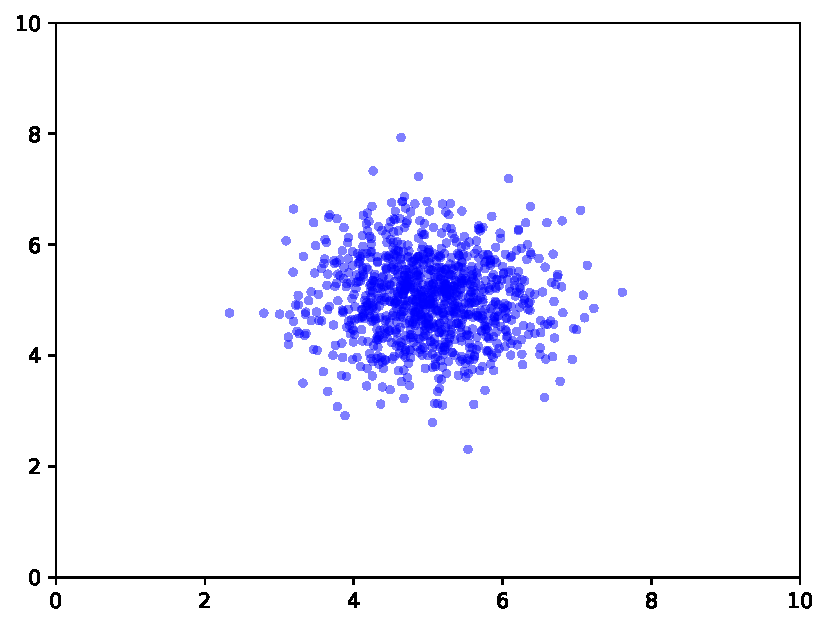
\includegraphics[width=0.19\linewidth]{figures/old/exp_multi_observation_base_N_3_gt_samples}
  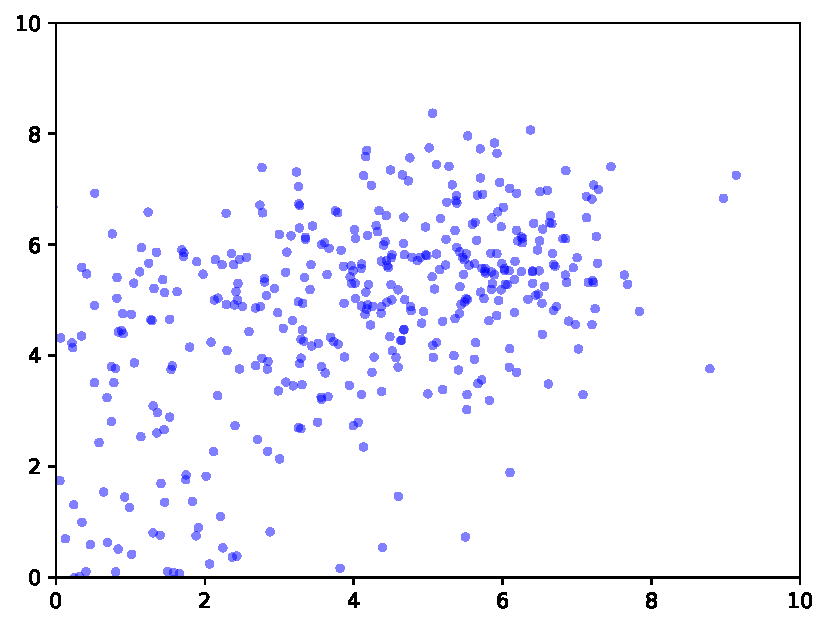
\includegraphics[width=0.19\linewidth]{figures/old/exp_multi_observation_base_N_3_npe_samples}
  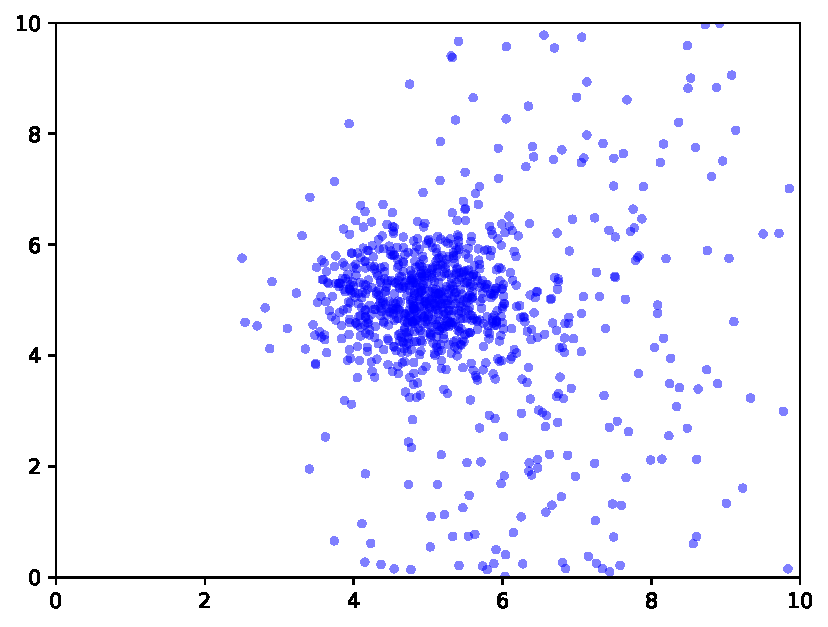
\includegraphics[width=0.19\linewidth]{figures/old/exp_multi_observation_base_N_3_nle_samples}
  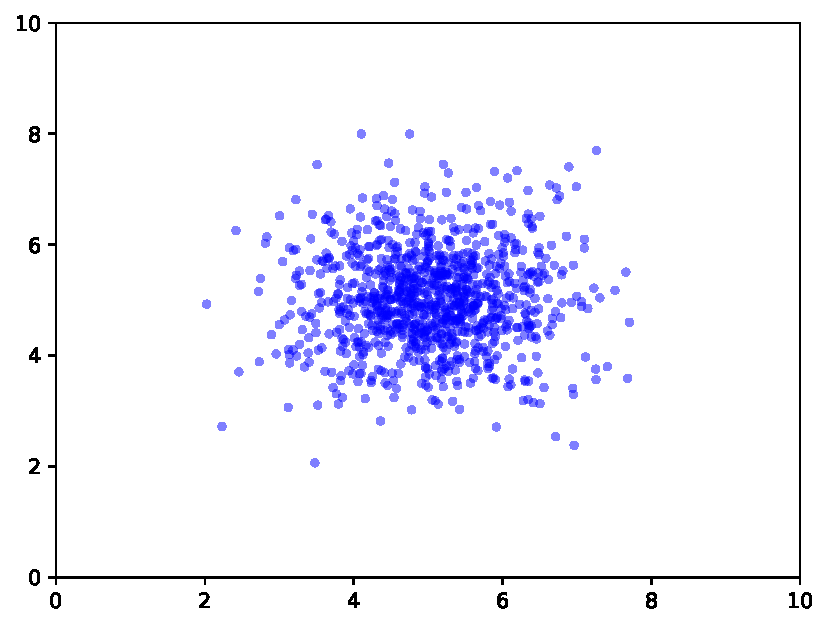
\includegraphics[width=0.19\linewidth]{figures/old/exp_multi_observation_base_N_3_romc_samples}
  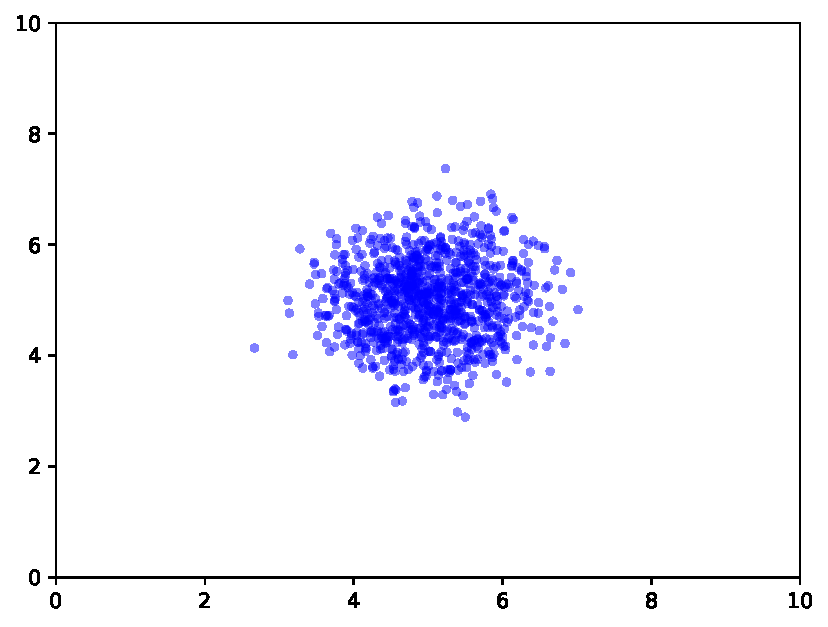
\includegraphics[width=0.19\linewidth]{figures/old/exp_multi_observation_base_N_3_r2omc_samples}\\
  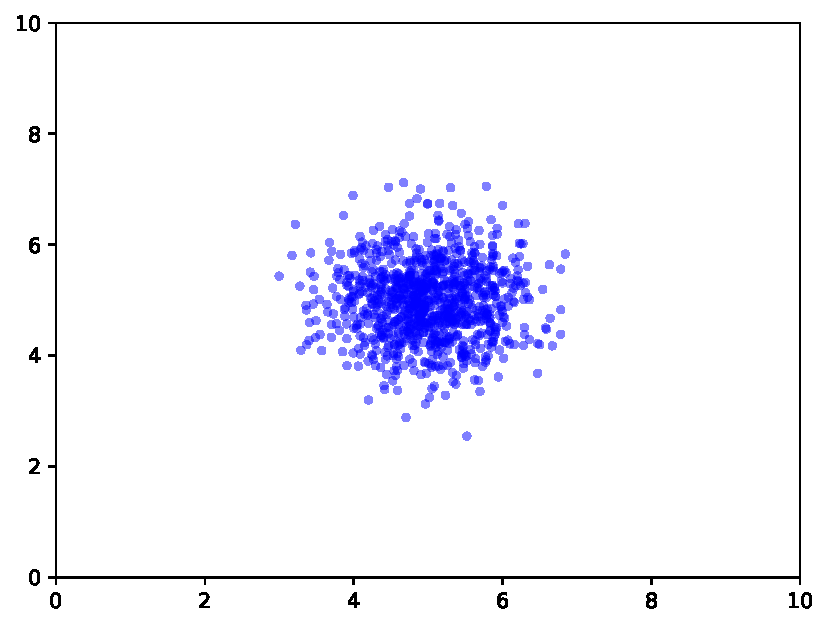
\includegraphics[width=0.19\linewidth]{figures/old/exp_multi_observation_base_N_5_gt_samples}
  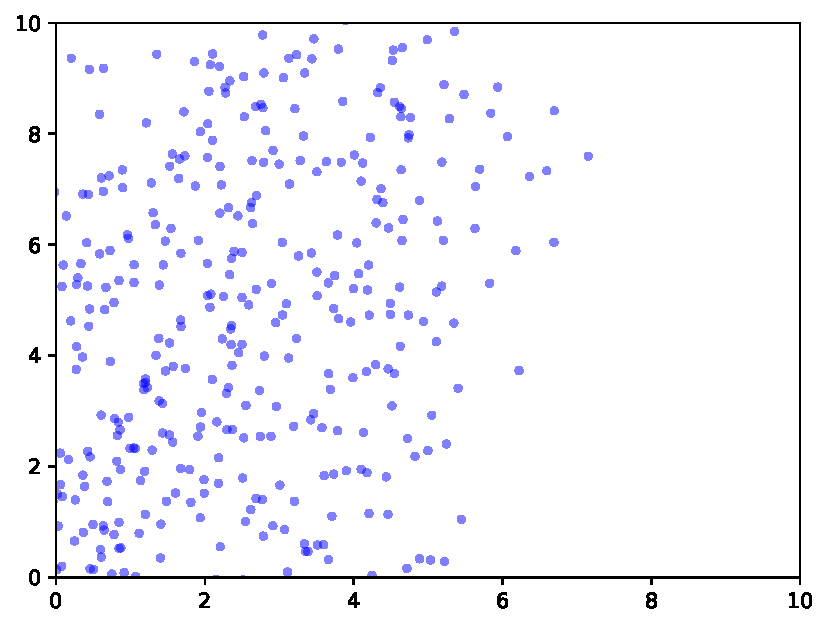
\includegraphics[width=0.19\linewidth]{figures/old/exp_multi_observation_base_N_5_npe_samples}
  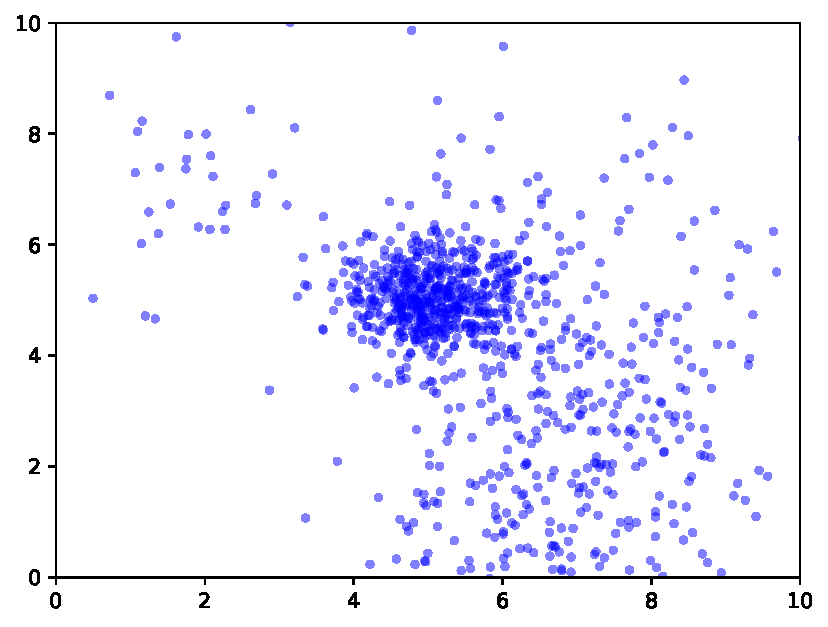
\includegraphics[width=0.19\linewidth]{figures/old/exp_multi_observation_base_N_5_nle_samples}
  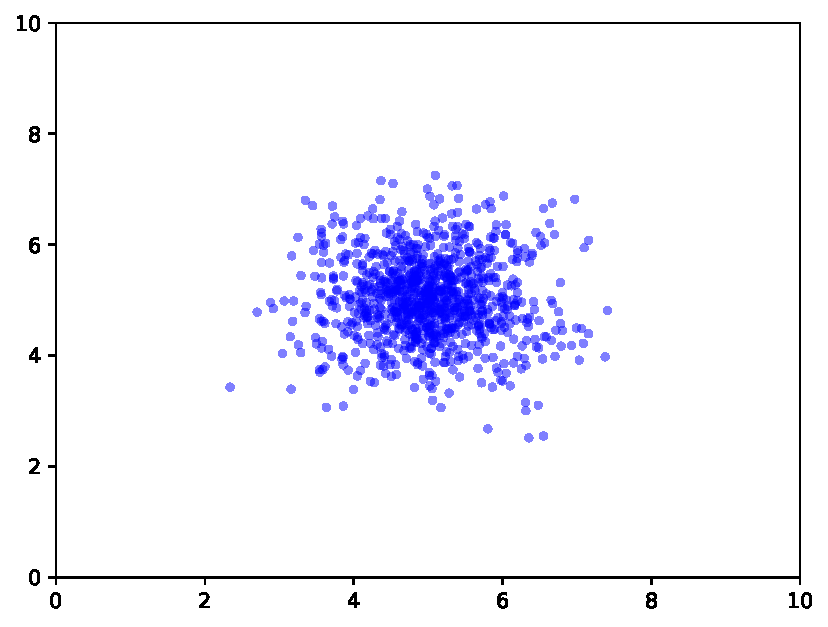
\includegraphics[width=0.19\linewidth]{figures/old/exp_multi_observation_base_N_5_romc_samples}
  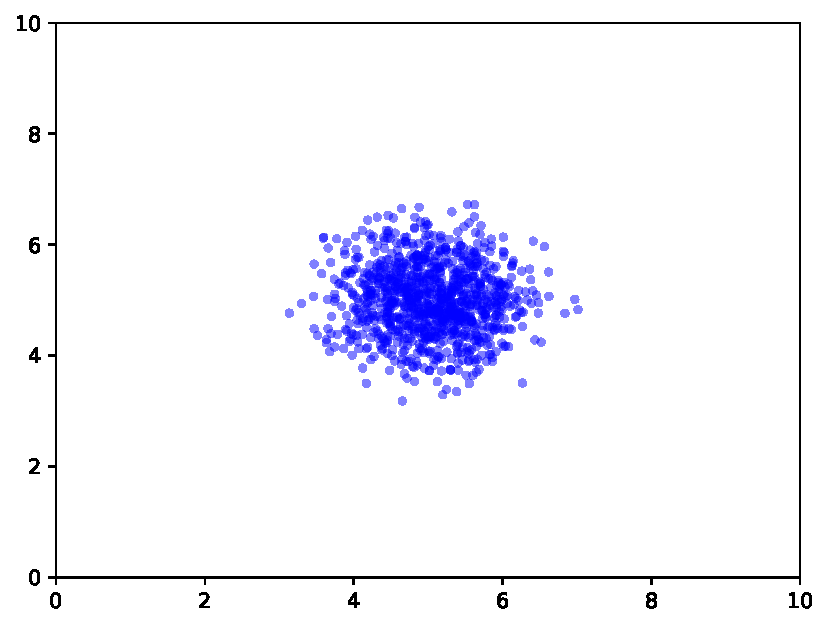
\includegraphics[width=0.19\linewidth]{figures/old/exp_multi_observation_base_N_5_r2omc_samples}\\
  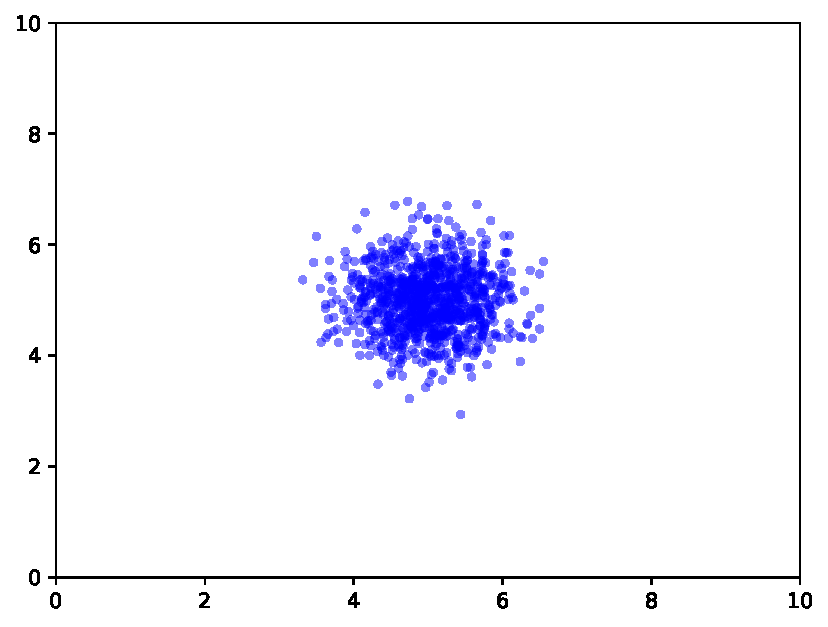
\includegraphics[width=0.19\linewidth]{figures/old/exp_multi_observation_base_N_10_gt_samples}
  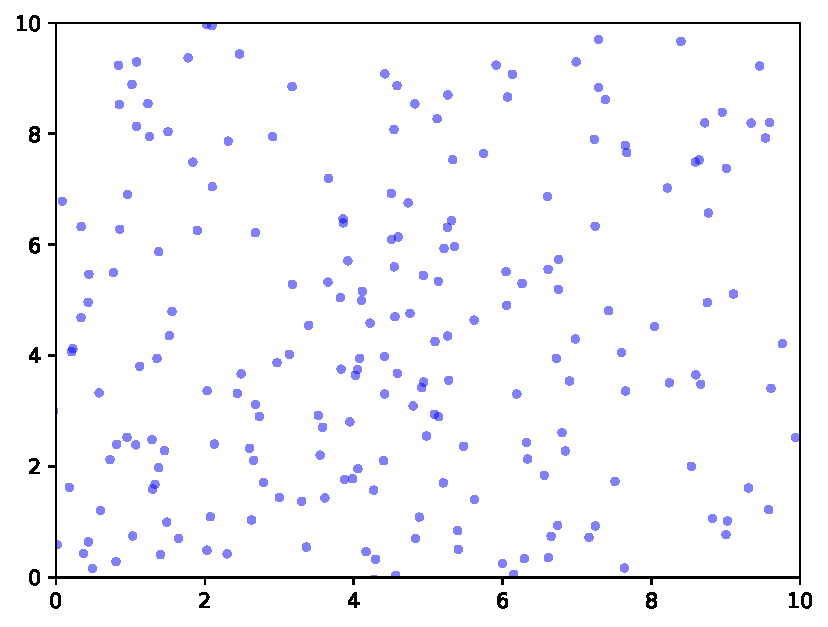
\includegraphics[width=0.19\linewidth]{figures/old/exp_multi_observation_base_N_10_npe_samples}
  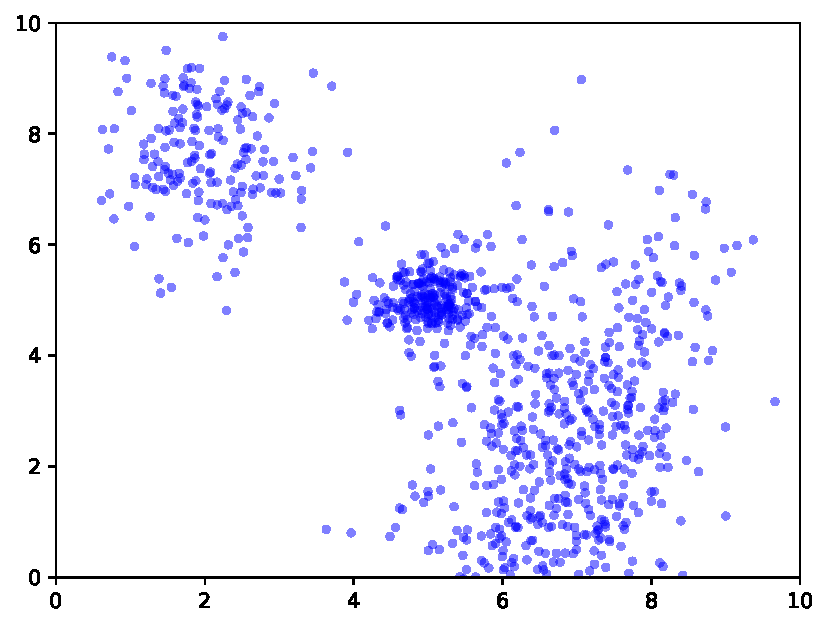
\includegraphics[width=0.19\linewidth]{figures/old/exp_multi_observation_base_N_10_nle_samples}
  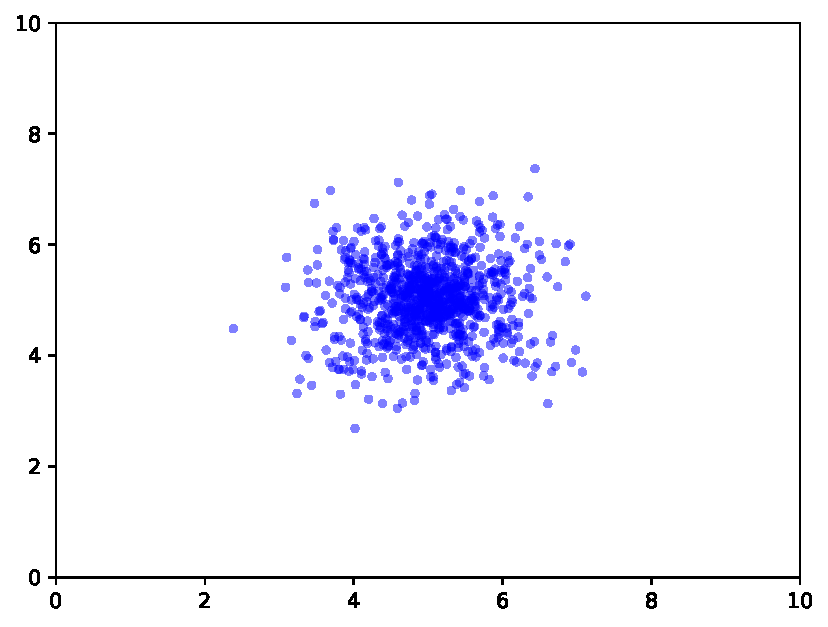
\includegraphics[width=0.19\linewidth]{figures/old/exp_multi_observation_base_N_10_romc_samples}
  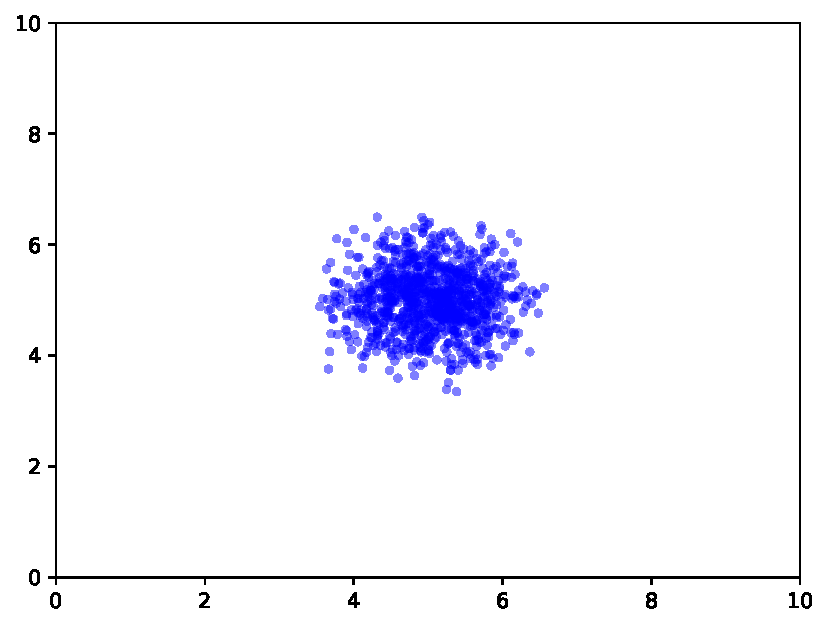
\includegraphics[width=0.19\linewidth]{figures/old/exp_multi_observation_base_N_10_r2omc_samples}\\
  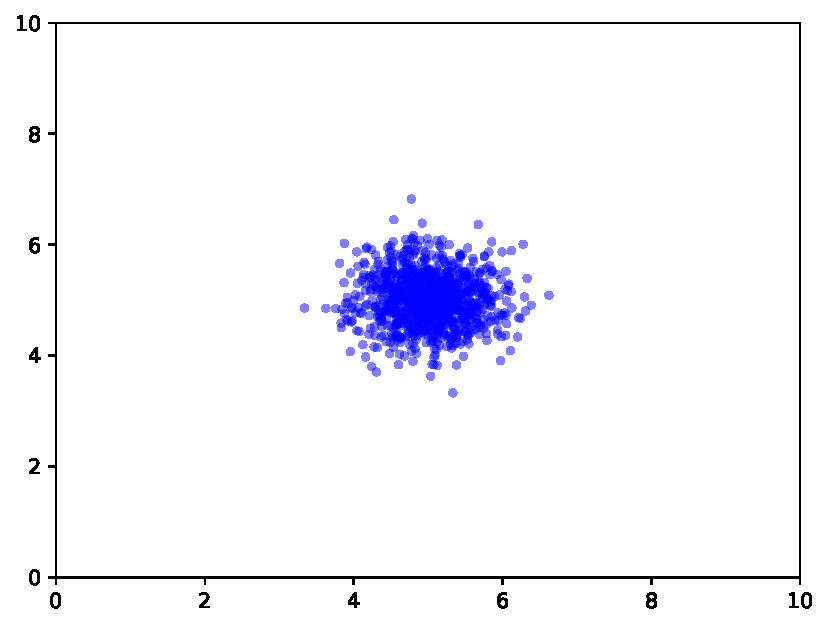
\includegraphics[width=0.19\linewidth]{figures/old/exp_multi_observation_base_N_20_gt_samples}
  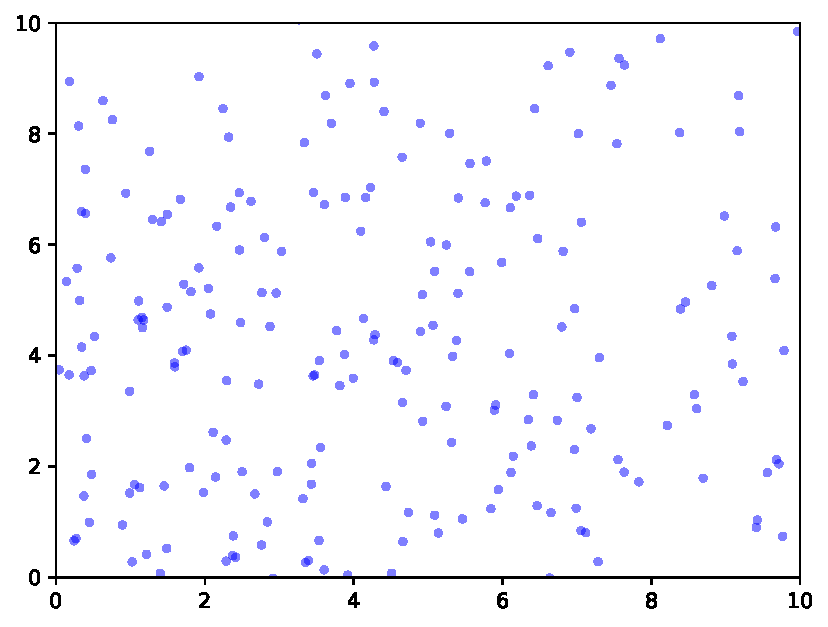
\includegraphics[width=0.19\linewidth]{figures/old/exp_multi_observation_base_N_20_npe_samples}
  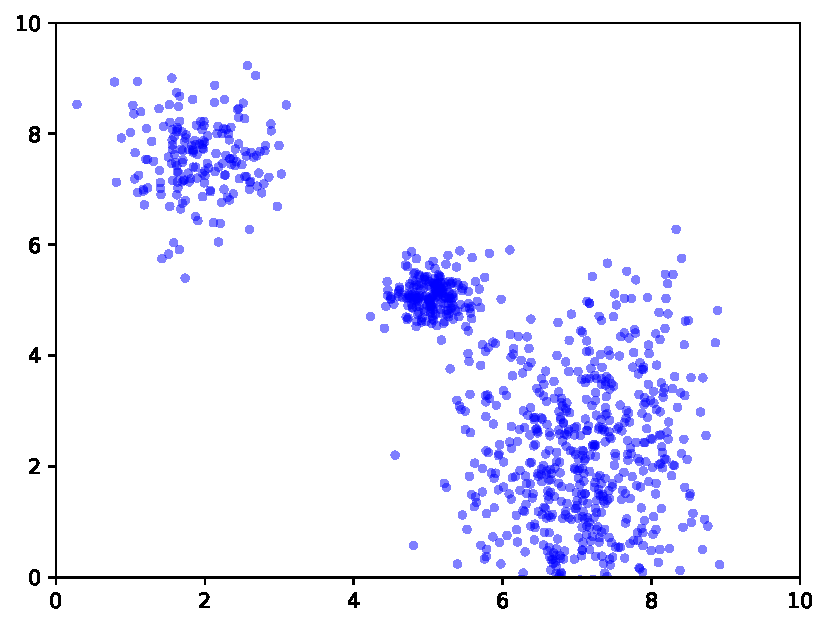
\includegraphics[width=0.19\linewidth]{figures/old/exp_multi_observation_base_N_20_nle_samples}
  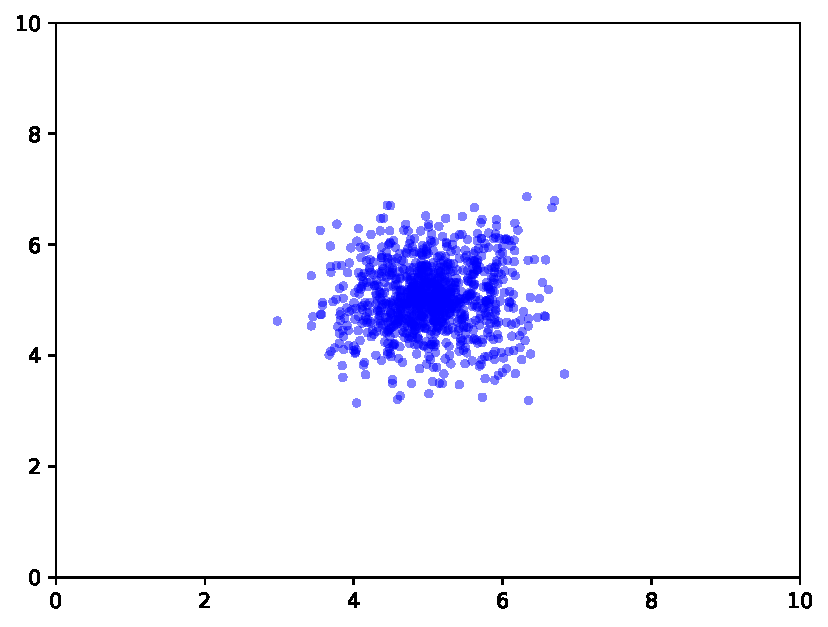
\includegraphics[width=0.19\linewidth]{figures/old/exp_multi_observation_base_N_20_romc_samples}
  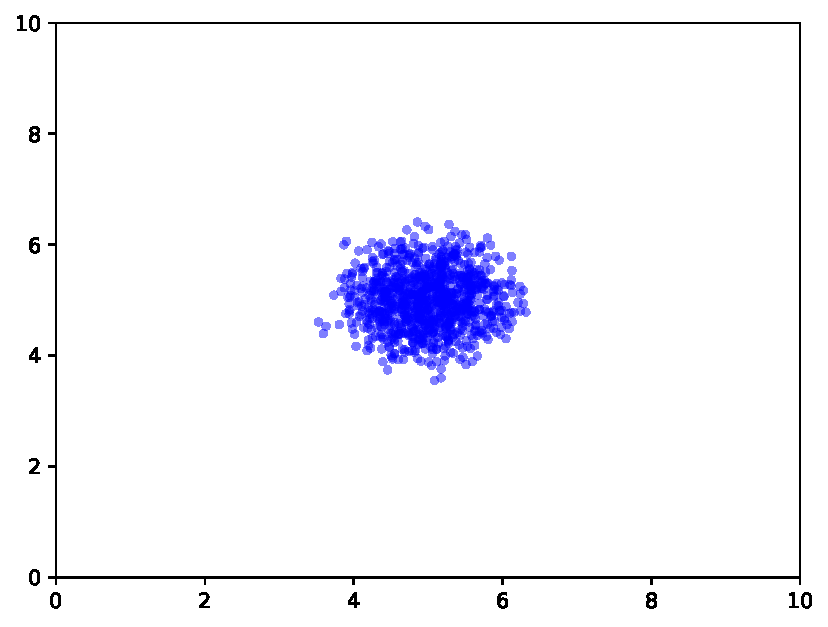
\includegraphics[width=0.19\linewidth]{figures/old/exp_multi_observation_base_N_20_r2omc_samples}
  \caption{Multi observations Base: Left to right: ground truth, NPE, NLE, Naive-ROMC, R2OMC. Top to bottom: $N=3$, $N=5$, $N=10$, $N=10$}
  \label{fig:mo_multi_obs_base}
\end{figure}


\subsubsection{MoG simulator}

\begin{tabular}{@{}ll@{}}
  \textbf{Prior} & $\thb \sim \mathcal{U}(-\mathbf{15}, \mathbf{15})$ \\ [5pt]
  \textbf{Simulator} & $\yb \sim \frac{1}{2} \left( \mathcal{N}(\thb, \sigma_1^2 \mathbf{I}) + \mathcal{N}(-\thb, \sigma_2^2 \mathbf{I}) \right)$, with $\sigma_1=\sigma_2=1$ \\ [5pt]
  \textbf{Dimensionality} & $\thb \in \mathbb{R}^{D}$, $\yb \in \mathbb{R}^{D}$ \\ [5pt]
  \textbf{Observations} & $\{\data_n\}_n^N$ where: \\ [5pt]
  & $\data_n = (5, \ldots, 5) + \epsilon$ for $n \in \{1, \ldots, \frac{N}{2}\}$, \\ [5pt] 
  & $\data_n = (-5, \ldots, -5) + \epsilon$ for $n \in \{\frac{N}{2}+1, \ldots, N\}$ \\ [5pt]
  \textbf{Posterior} & $ p(\thb | \data) \propto
                                    \begin{cases}
                                      \mathcal{N}(\thb; \mathbf{5}, \frac{1}{N} \mathbf{I}) + \mathcal{N}(\thb; -\mathbf{5}, \frac{1}{N} \mathbf{I}), & \text{if } \thb \in [-15, 15]^D, \\
                                      0, & \text{otherwise}.
                                    \end{cases} $ \\ [5pt]
\end{tabular}

\textbf{Proof of the posterior:}
\begin{equation}
  p(\thb|\{\data_n\}) \appropto 
  \begin{cases}
    \mathcal{N}(\thb; \mathbf{5}, \frac{1}{N} \mathbf{I}) + \mathcal{N}(\thb; -\mathbf{5}, \frac{1}{N}\mathbf{I}), & \text{if } \thb \in [-15, 15]^D, \\
    0, & \text{otherwise}.
  \end{cases}
  \label{eq:mog_mog_mult_obs}
\end{equation}
The proof is similar to the one in Eq.~(\ref{eq:intro-multiple}).

In Figure~\ref{fig:mog_multi_obs}, we present the results for the MoG simulator with multiple observations.


\begin{figure}[]
  \centering
  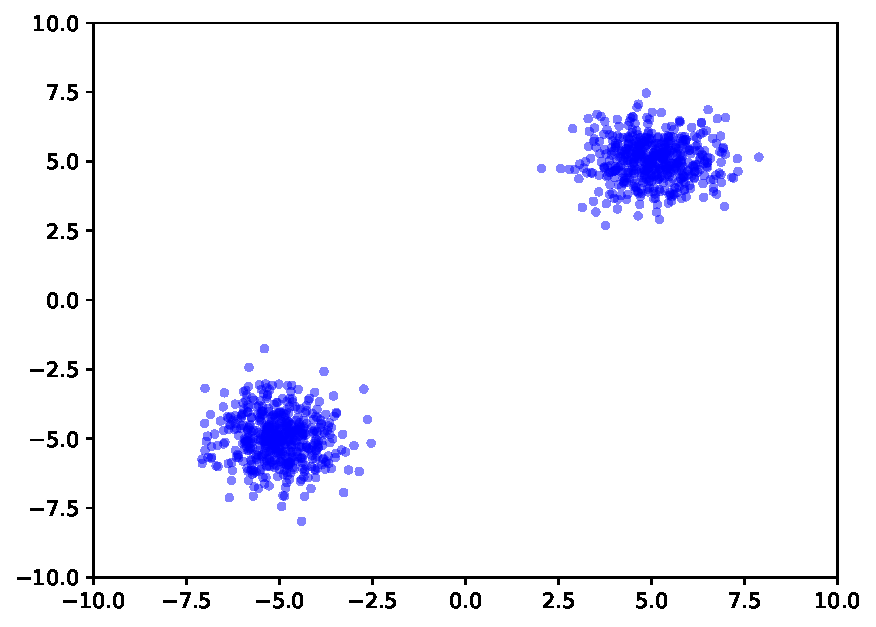
\includegraphics[width=0.19\linewidth]{figures/old/exp_multi_observation_MoG_N_2_gt_samples}
  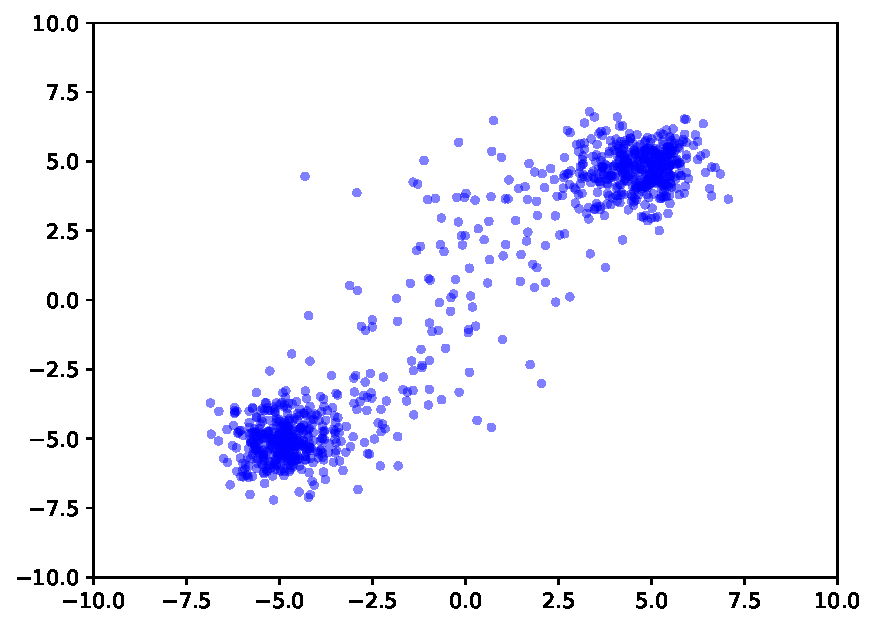
\includegraphics[width=0.19\linewidth]{figures/old/exp_multi_observation_MoG_N_2_npe_samples}
  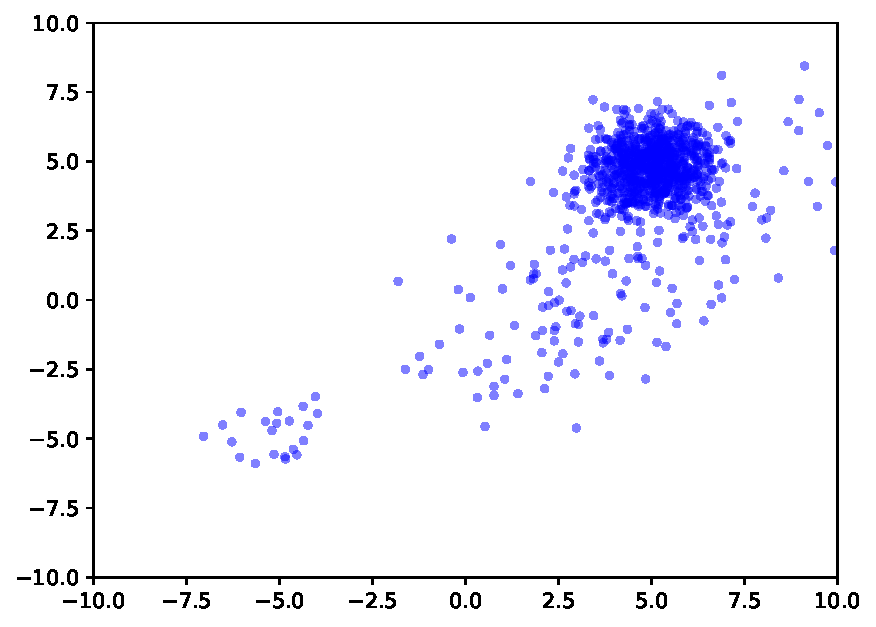
\includegraphics[width=0.19\linewidth]{figures/old/exp_multi_observation_MoG_N_2_nle_samples}
  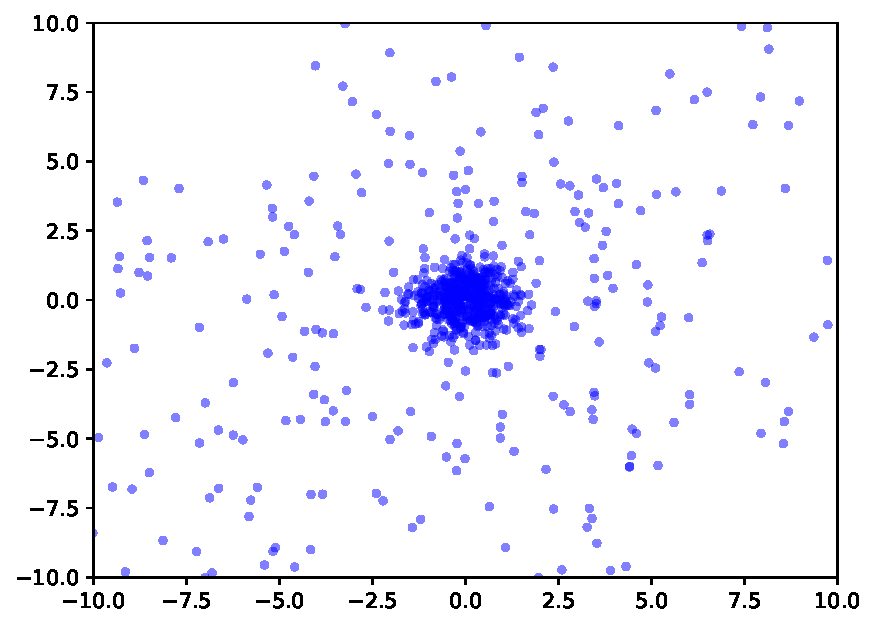
\includegraphics[width=0.19\linewidth]{figures/old/exp_multi_observation_MoG_N_2_romc_samples}
  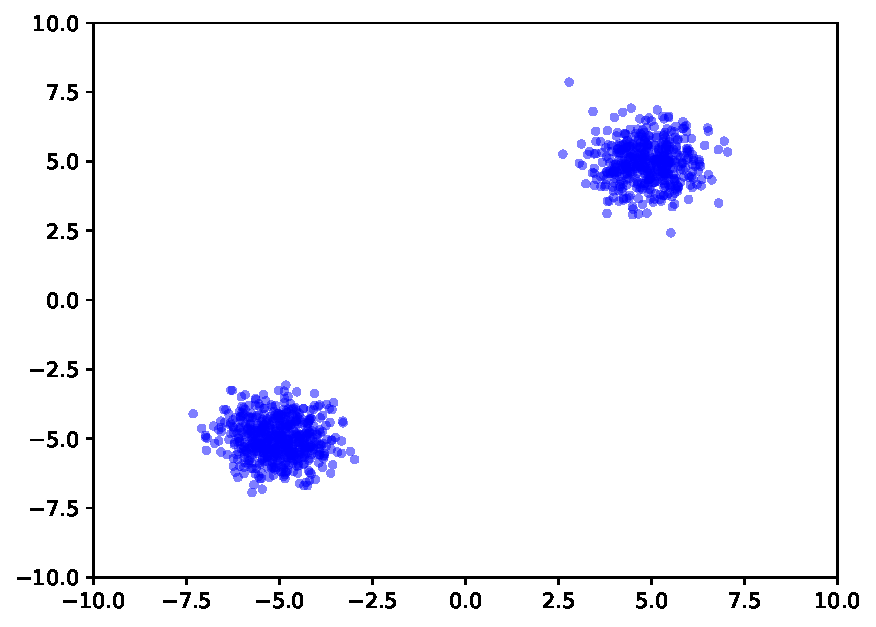
\includegraphics[width=0.19\linewidth]{figures/old/exp_multi_observation_MoG_N_2_r2omc_samples}\\
  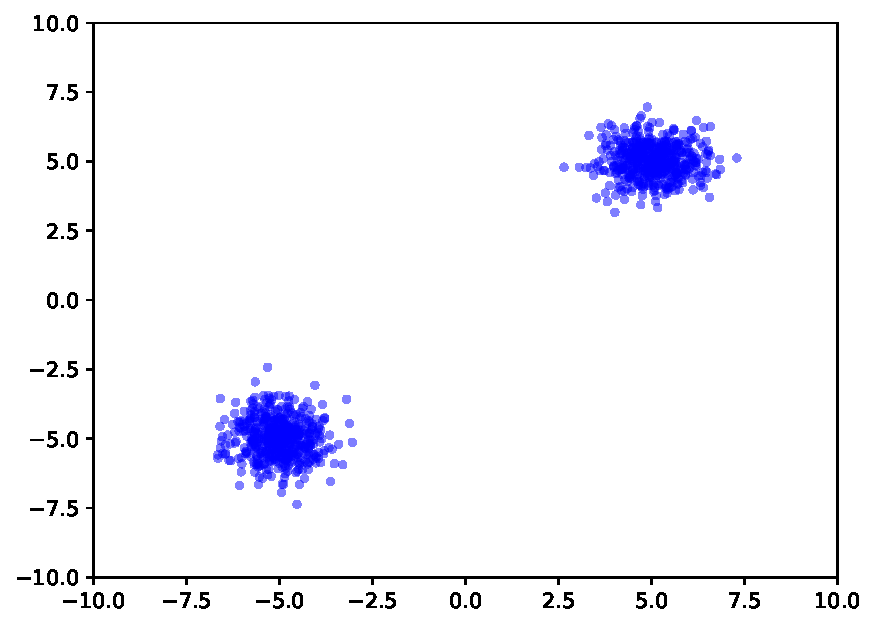
\includegraphics[width=0.19\linewidth]{figures/old/exp_multi_observation_MoG_N_5_gt_samples}
  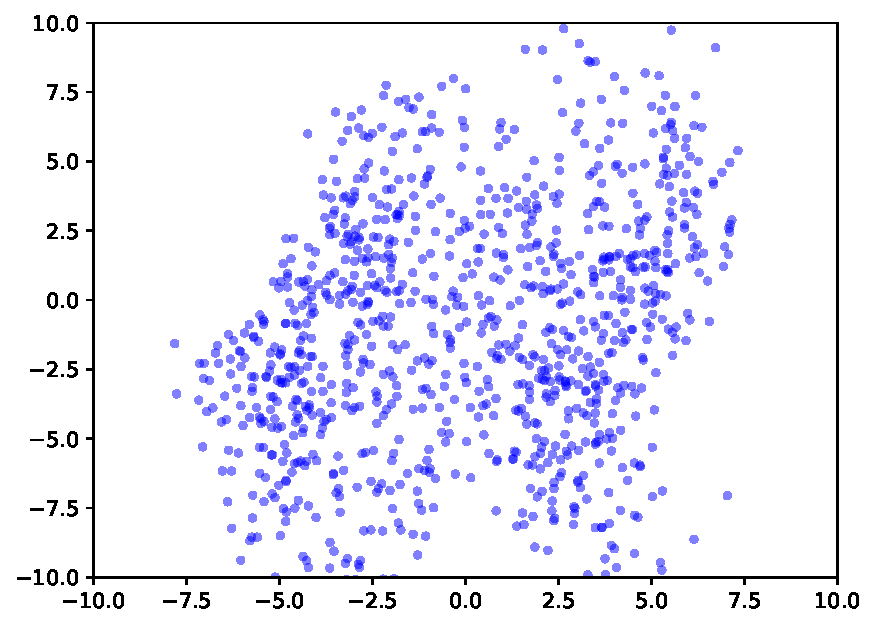
\includegraphics[width=0.19\linewidth]{figures/old/exp_multi_observation_MoG_N_5_npe_samples}
  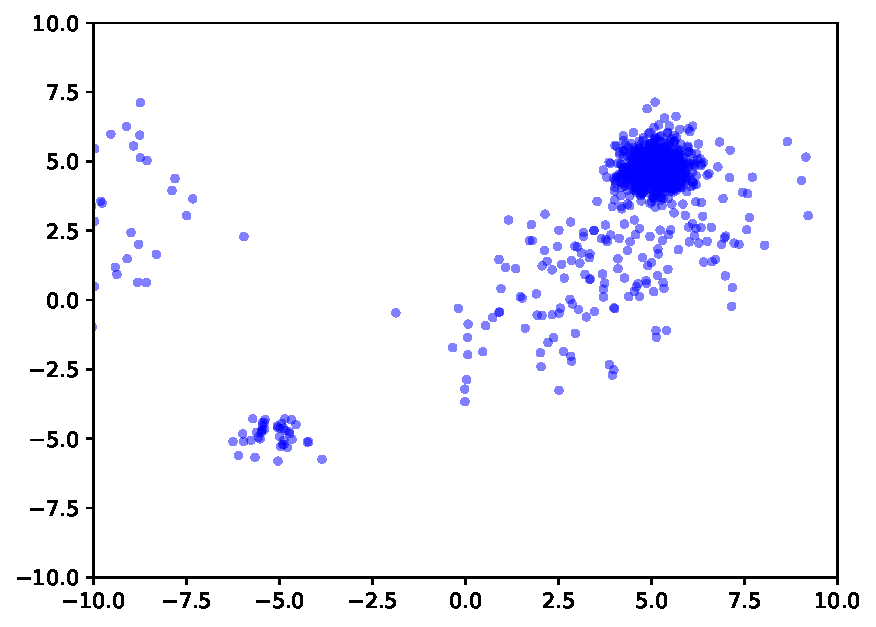
\includegraphics[width=0.19\linewidth]{figures/old/exp_multi_observation_MoG_N_5_nle_samples}
  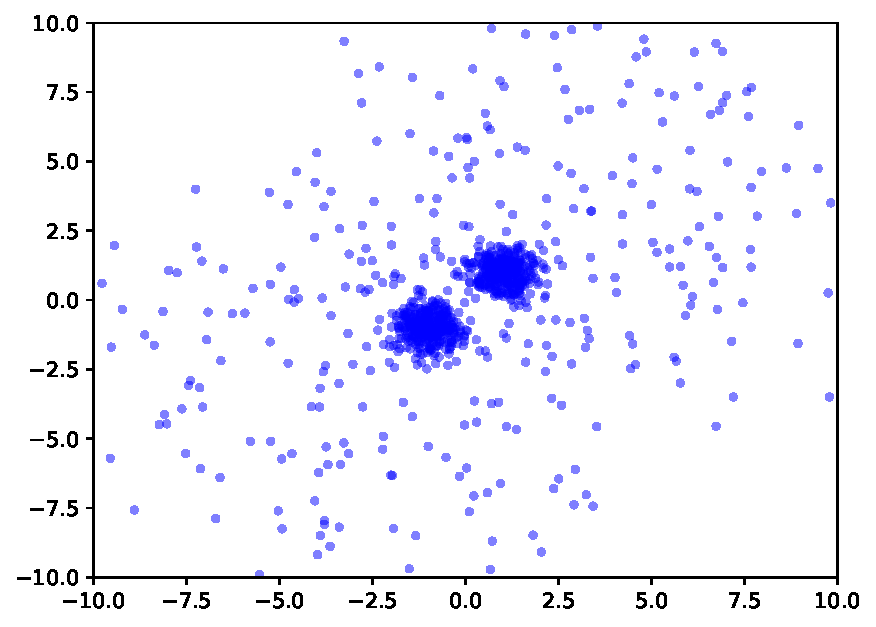
\includegraphics[width=0.19\linewidth]{figures/old/exp_multi_observation_MoG_N_5_romc_samples}
  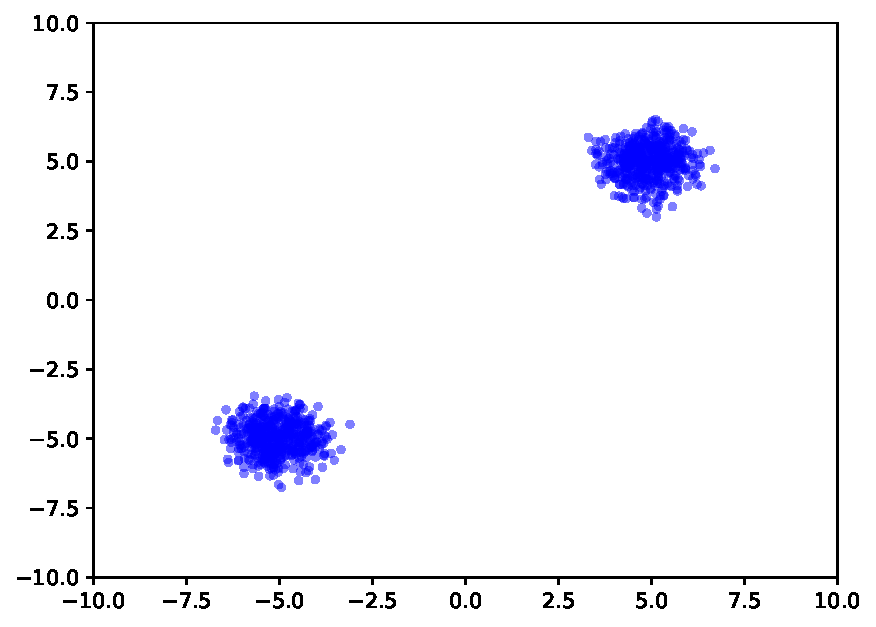
\includegraphics[width=0.19\linewidth]{figures/old/exp_multi_observation_MoG_N_5_r2omc_samples}\\
  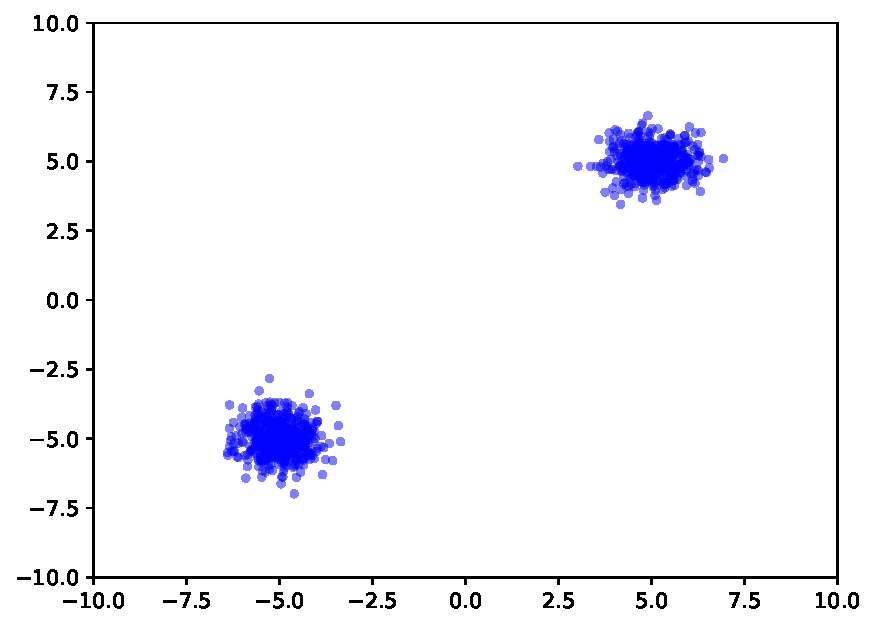
\includegraphics[width=0.19\linewidth]{figures/old/exp_multi_observation_MoG_N_10_gt_samples}
  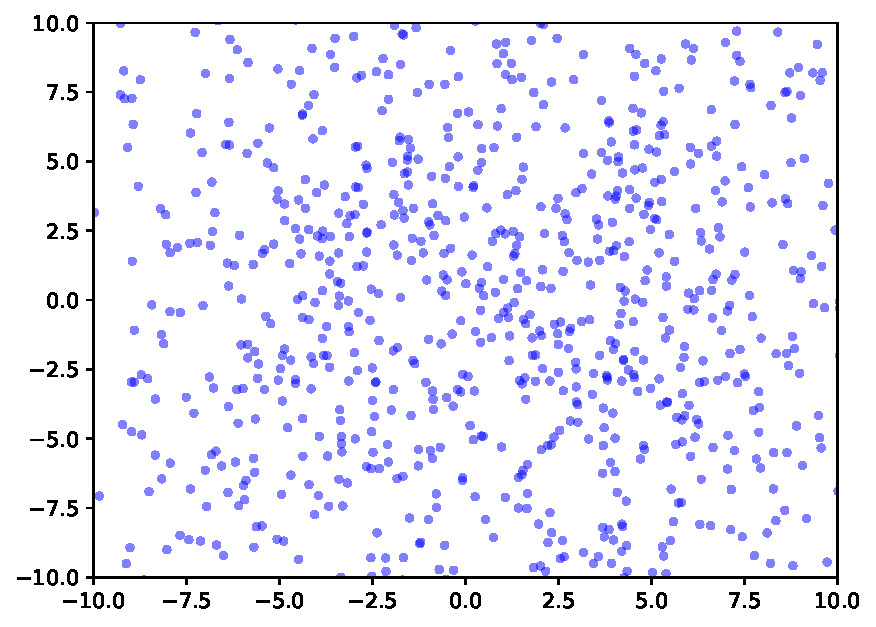
\includegraphics[width=0.19\linewidth]{figures/old/exp_multi_observation_MoG_N_10_npe_samples}
  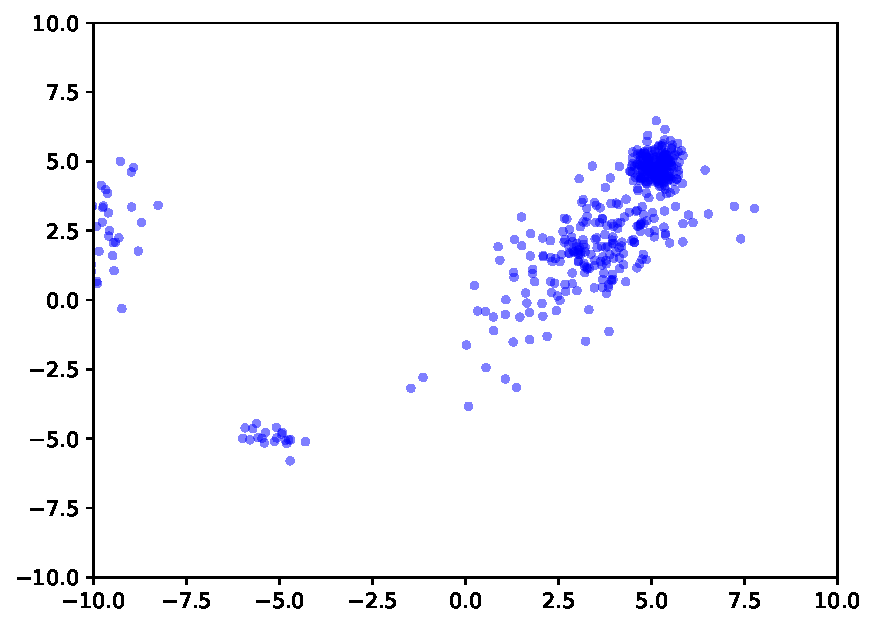
\includegraphics[width=0.19\linewidth]{figures/old/exp_multi_observation_MoG_N_10_nle_samples}
  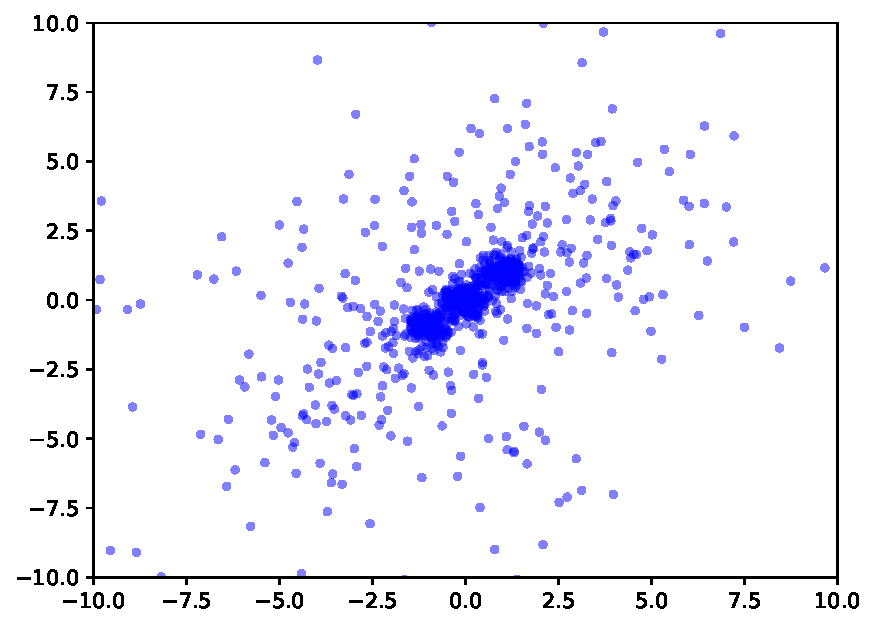
\includegraphics[width=0.19\linewidth]{figures/old/exp_multi_observation_MoG_N_10_romc_samples}
  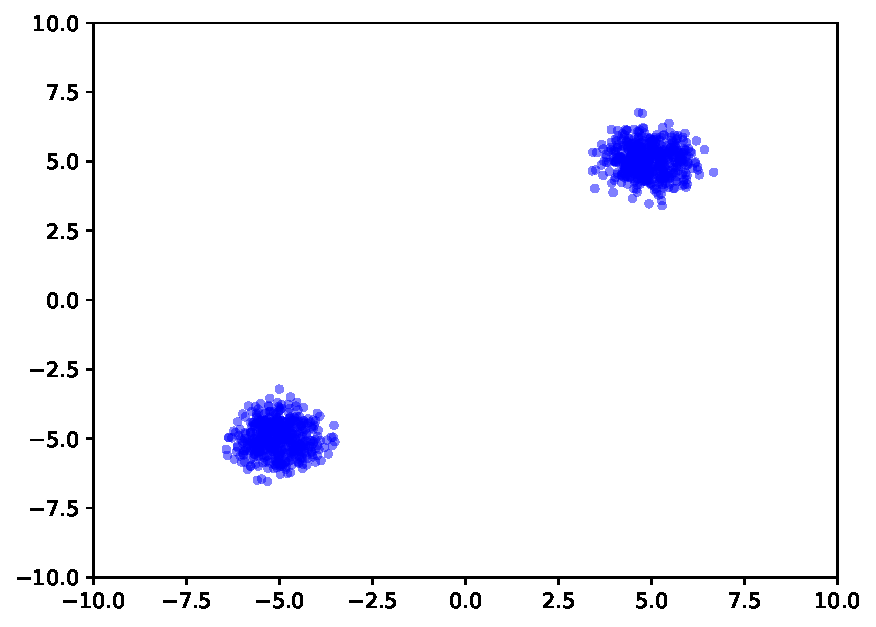
\includegraphics[width=0.19\linewidth]{figures/old/exp_multi_observation_MoG_N_10_r2omc_samples}\\
  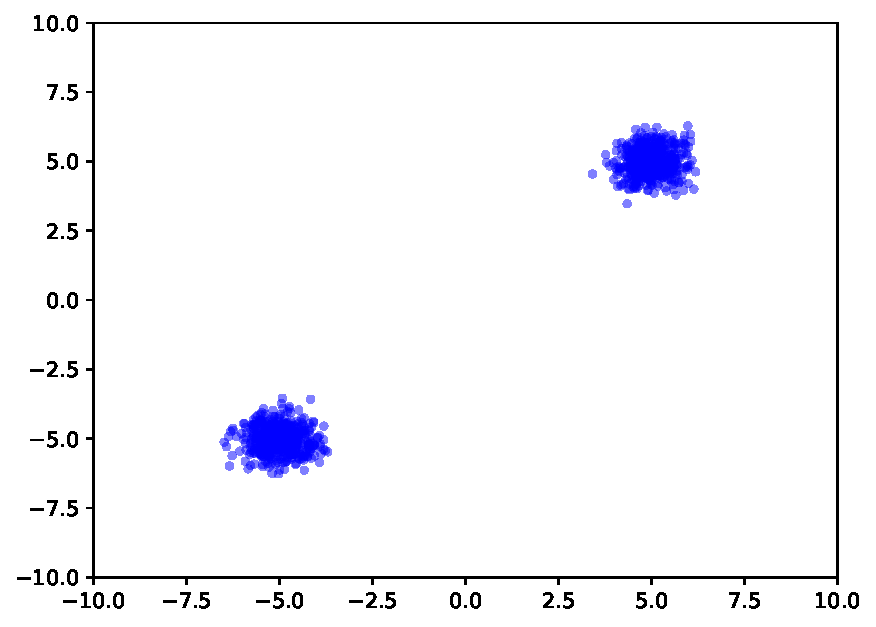
\includegraphics[width=0.19\linewidth]{figures/old/exp_multi_observation_MoG_N_20_gt_samples}
  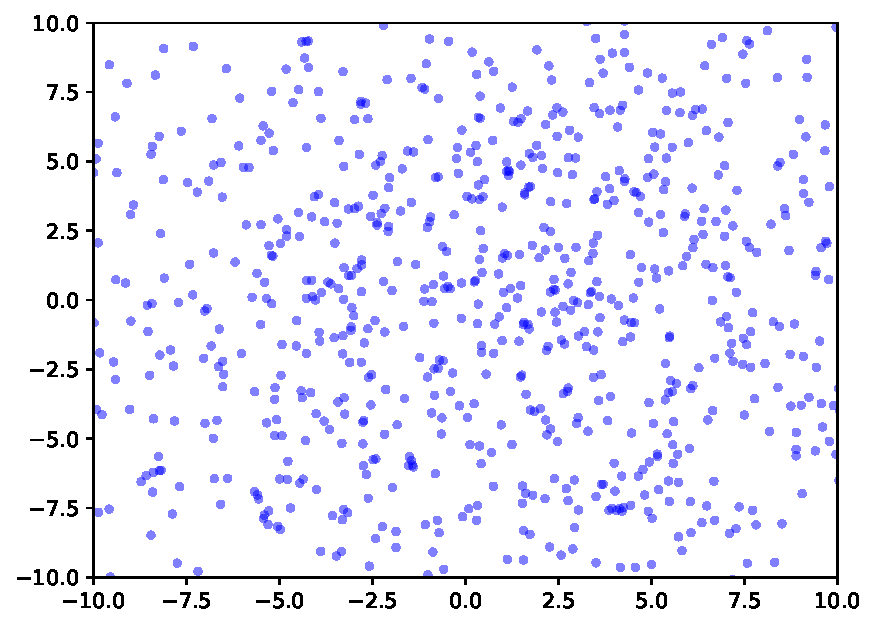
\includegraphics[width=0.19\linewidth]{figures/old/exp_multi_observation_MoG_N_20_npe_samples}
  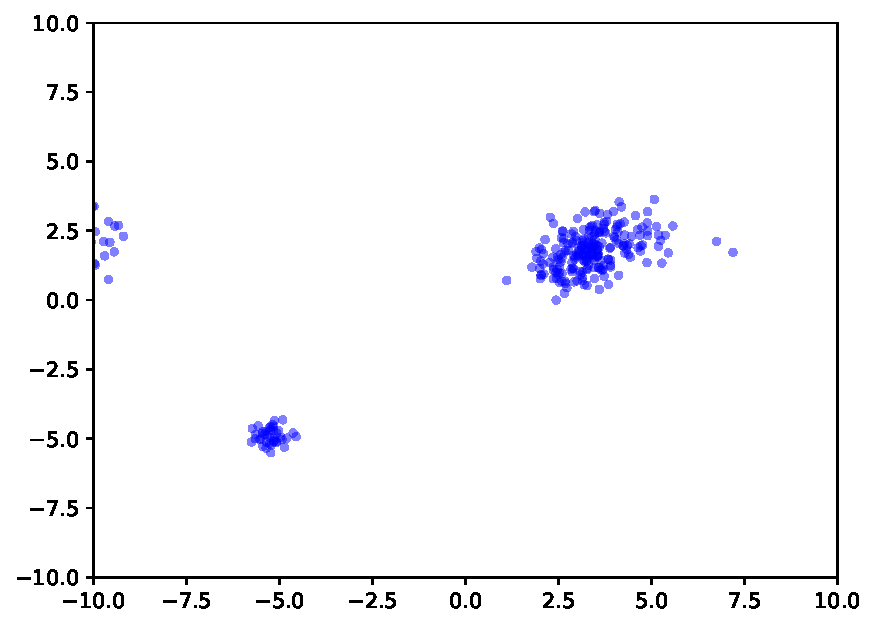
\includegraphics[width=0.19\linewidth]{figures/old/exp_multi_observation_MoG_N_20_nle_samples}
  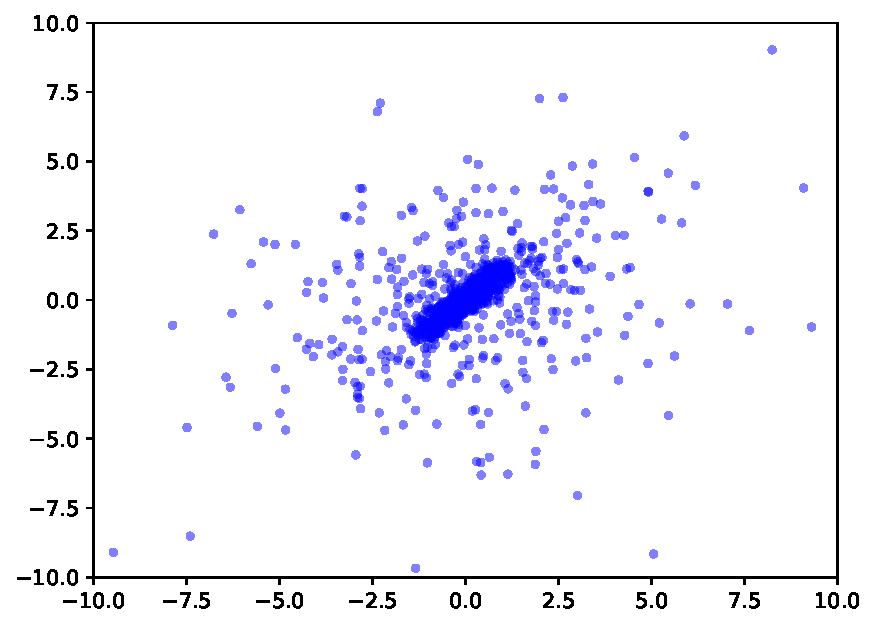
\includegraphics[width=0.19\linewidth]{figures/old/exp_multi_observation_MoG_N_20_romc_samples}
  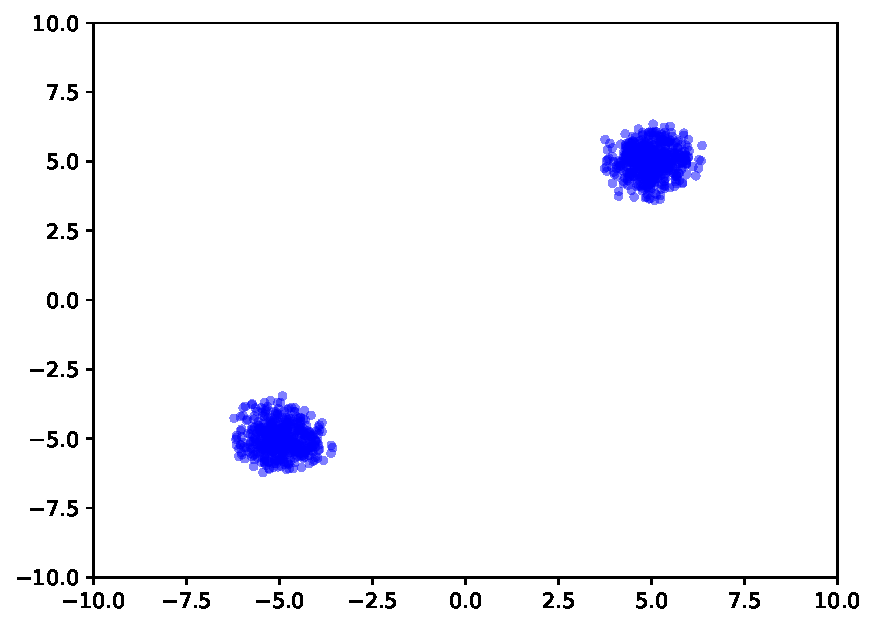
\includegraphics[width=0.19\linewidth]{figures/old/exp_multi_observation_MoG_N_20_r2omc_samples}
  \caption{Multi observations MoG: Left to right: ground truth, NPE, NLE, Naive-ROMC, R2OMC. Top to bottom: $N=3$, $N=5$, $N=10$, $N=10$}
  \label{fig:mog_multi_obs}
\end{figure}

\subsection{SBI - Mixtures of Gaussians (T.7)}

We here provide additional information on example T.7 of the SBI benchmark~\cite{lueckmann2021benchmarking}.
It tests inference of the mean of a mixture of two $2$-D Gaussians, one with much broader covariance than the other

\begin{tabular}{@{}ll@{}}
  \textbf{Prior} & $\thb \sim \mathcal{U}(-\mathbf{10}, \mathbf{10})$ \\ [5pt]
  \textbf{Simulator} & $\yb \sim 0.5 (\mathcal{N}(\thb, \mathbf{I}) + \mathcal{N}(\thb, \sigma^2 \mathbf{I}))$, with $\sigma^2 = 0.01$ \\ [5pt]
  \textbf{Dimensionality} & $\thb \in \mathbb{R}^{2}$, $\yb \in \mathbb{R}^{2}$ \\ [5pt]
\end{tabular}

\paragraph{Results.}

We evaluate \rromc~using a simulation budget of $S=1000$ and $S=10000$ seeds.
The \texttt{C2ST} score is computed by comparing 1000 samples from the true posterior (we randomly select 1000 from the 10000 that are provided by the SBI benchmark)
with 1000 samples generated from the \rromc~approximate posterior.
The results are illustrated in Figure~\ref{fig:exp_sbi_gaussian_mixture}.

\begin{figure}[ht]
  \centering
  \begin{subfigure}[b]{0.32\linewidth}
    \centering
    \includegraphics[width=\linewidth]{figures/old/gaussian_mixture}
    \caption{\texttt{C2ST} score}
  \end{subfigure}
  \hfill
  \begin{subfigure}[b]{0.32\linewidth}
    \centering
    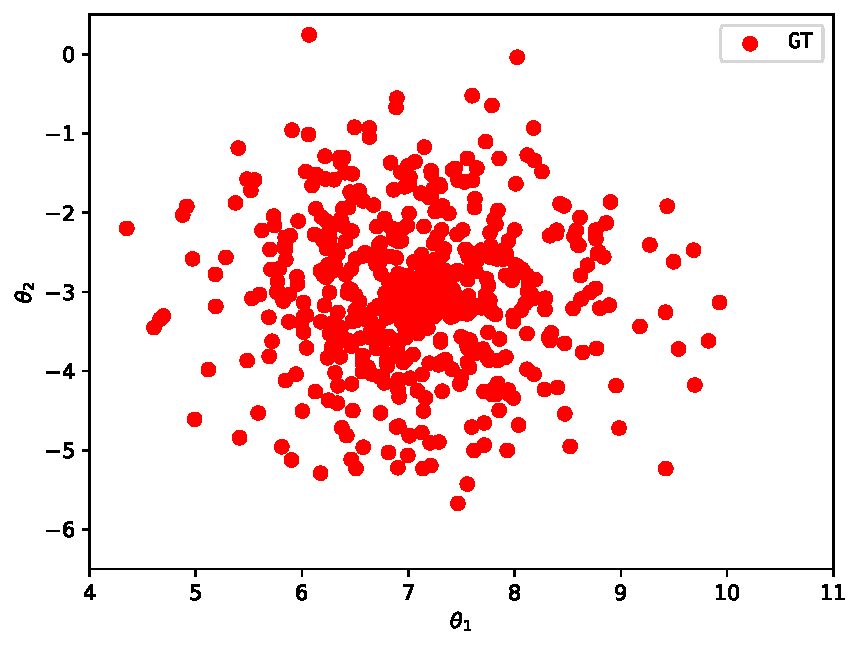
\includegraphics[width=\linewidth]{figures/old/exp_sbi_gaussian_mixture_gt}
    \caption{Ground truth samples}
  \end{subfigure}
  \hfill
  \begin{subfigure}[b]{0.32\linewidth}
    \centering
    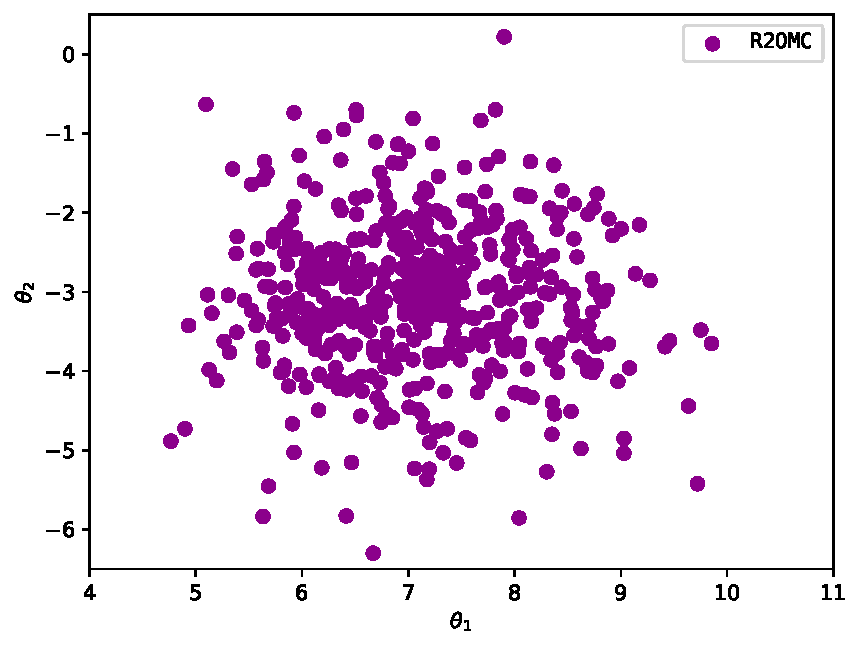
\includegraphics[width=\linewidth]{figures/old/exp_sbi_gaussian_mixture_r2omc}
    \caption{Samples by R2OMC}
  \end{subfigure}
  \caption{T.7: Gaussian Mixture. From left to right: \texttt{C2ST} score, ground truth samples, and samples by R2OMC.}
  \label{fig:exp_sbi_gaussian_mixture}
\end{figure}

\subsection{SBI - Two Moons (T.8)}

We here provide additional information on example T.8 of the SBI benchmark~\cite{lueckmann2021benchmarking}.
It tests inference when the posterior exhibits both global (bimodality) and local (crescent shape) structure to illustrate how algorithms deal with multimodality:

\begin{tabular}{@{}ll@{}}
  \textbf{Prior} & $\thb \sim \mathcal{U}(-\mathbf{1}, \mathbf{1})$ \\ [5pt]
  \textbf{Simulator} & $\yb \sim \begin{bmatrix} 
    r \cos(\alpha) + 0.25 \\ 
    r \sin(\alpha)
  \end{bmatrix} + \begin{bmatrix} 
    |\theta_1 + \theta_2|/\sqrt{2} \\ 
    (-\theta_1 + \theta_2)/\sqrt{2}
  \end{bmatrix}$, where $r \sim \mathcal{N}(0.1, 0.01^2)$ and $\alpha \sim \mathcal{U}(-\pi/2, \pi/2)$ \\ [10pt]
  \textbf{Dimensionality} & $\thb \in \mathbb{R}^{2}$, $\yb \in \mathbb{R}^{2}$ \\ [5pt]
\end{tabular}

\paragraph{Results.}

We evaluate \rromc~using a simulation budget of $S=1000$ and $S=10000$ seeds.
The \texttt{C2ST} score is computed by comparing 1000 samples from the true posterior (we randomly select 1000 from the 10000 that are provided by the SBI benchmark)
with 1000 samples generated from the \rromc~approximate posterior.
The results are illustrated in Figure~\ref{fig:exp_sbi_gaussian_mixture}.
We observe that \rromc~is able to capture the bimodal structure of the posterior, perfectly replicating the ground truth samples.

\begin{figure}[ht]
  \centering
  \begin{subfigure}[b]{0.32\linewidth}
    \centering
    \includegraphics[width=\linewidth]{figures/old/two_moons}
    \caption{\texttt{C2ST} score}
  \end{subfigure}
  \hfill
  \begin{subfigure}[b]{0.32\linewidth}
    \centering
    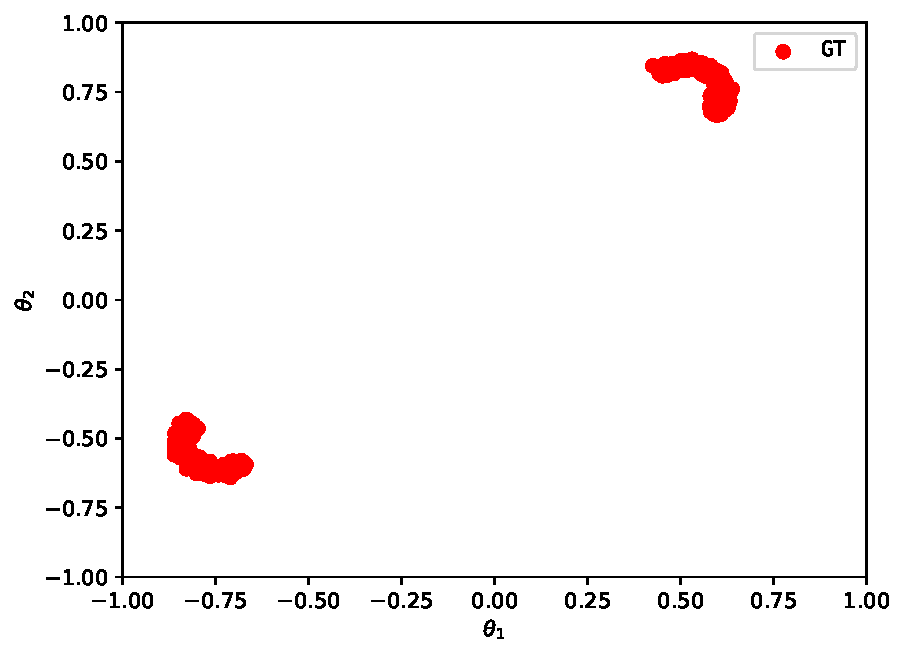
\includegraphics[width=\linewidth]{figures/old/exp_sbi_two_moons_gt}
    \caption{Ground truth samples}
  \end{subfigure}
  \hfill
  \begin{subfigure}[b]{0.32\linewidth}
    \centering
    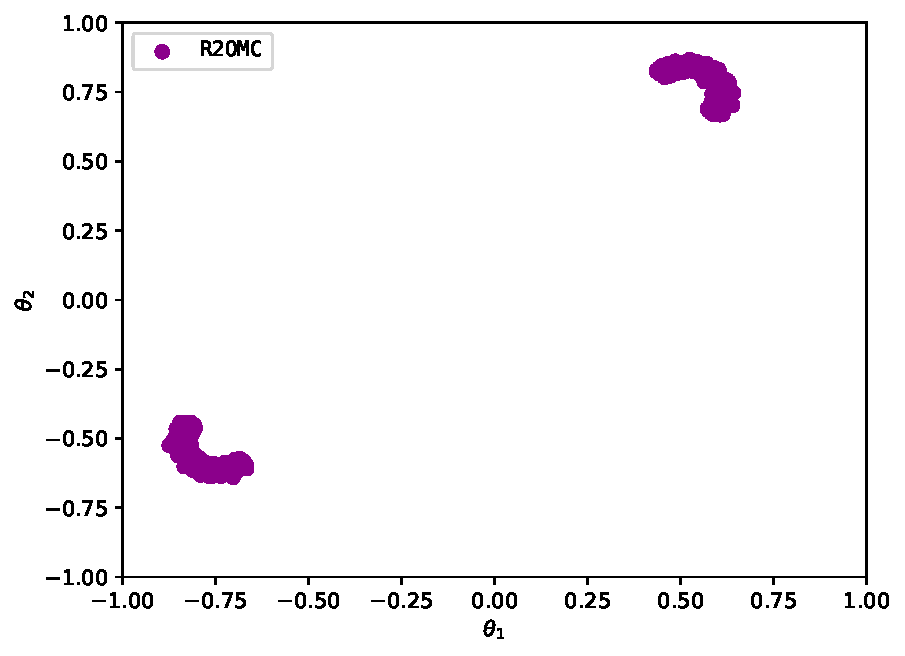
\includegraphics[width=\linewidth]{figures/old/exp_sbi_two_moons_r2omc}
    \caption{Samples by R2OMC}
  \end{subfigure}
  \caption{T.8: Two Moons. From left to right: \texttt{C2ST} score, ground truth samples, and samples by R2OMC.}
  \label{fig:exp_sbi_two_moons}
\end{figure}

\clearpage

\section{Additional results}
\label{sec:additional-experiments}

We here present some additional experiments that were not included in the main text.

% \subsection{SBI - Gaussian Linear Uniform (T.2)}

% This is the T.2 from the SBI benchmark~\cite{lueckmann2021benchmarking}.
% It tests inference of the mean of a $10$-D Gaussian model with fixed covariance.
% The posterior is a truncated Gaussian distribution:

% \begin{tabular}{@{}ll@{}}
%   \textbf{Prior} & $\thb \sim \mathcal{U}(-1, 1)$ \\[5pt]
%   \textbf{Simulator} & $\yb \sim \mathcal{N}(\thb, 0.1 \odot \mathbf{I})$ \\[5pt]
%   \textbf{Dimensionality} & $\thb \in \mathbb{R}^{10}$, $\yb \in \mathbb{R}^{10}$ \\[5pt]
% \end{tabular}

% \paragraph{Results.}

% We evaluate \rromc~using a simulation budget of $S=1000$ and $S=10000$ seeds.
% Running it for $S=100000$ seeds is omitted, as the \texttt{C2ST} score is almost $0.5$ (perfect score), even with just $S=1000$ seeds.
% The \texttt{C2ST} score is computed by comparing 1000 samples from the true posterior (we randomly select 1000 from the 10000 that are provided by the SBI benchmark)
% with 1000 samples generated from the \rromc~approximate posterior.
% The results are illustrated in Figure~\ref{fig:exp_sbi_extra} (Left).

% \subsection{SBI - SLCP (T.3)}

% This is the T.3 from the SBI benchmark~\cite{lueckmann2021benchmarking}.
% It is a challenging inference task designed to have a simple likelihood but a complex posterior.
% The prior is uniform over five parameters $\thb$ and the observations are four two-dimensional points sampled from a Gaussian likelihood
% whose mean and variance are nonlinear functions of $\thb$.

%\begin{tabular}{@{}ll@{}}
%   \textbf{Prior} & $\thb \sim \mathcal{U}(-3, 3)^5$ \\[5pt]
%   \textbf{Simulator} & $\mathbf{y} | \boldsymbol{\theta} \sim \mathcal{N}(\mathbf{m_{\theta}}, \mathbf{S_{\theta}}), \quad
%                        \mathbf{m_{\theta}} = \begin{bmatrix} \theta_1 \\ \theta_2 \end{bmatrix}, \quad
%                        \mathbf{S_{\theta}} = \begin{bmatrix} s_1^2 & \rho s_1 s_2 \\ \rho s_1 s_2 & s_2^2 \end{bmatrix},
%                        s_1 = \theta_3^2, s_2 = \theta_4^2, \rho = \tanh(\theta_5)$ \\[5pt]
%   \textbf{Dimensionality} & $\thb \in \mathbb{R}^{5}$, $\data_n \in \mathbb{R}^{2} \text{ for } n \in \{1, \ldots, 4\}$ \\[5pt] 
% \end{tabular}

% \paragraph{Results.}

% We evaluate \rromc~using a simulation budget of $S= \{1000, 10000, 100000\}$ seeds.
% The \texttt{C2ST} score is computed by comparing 1000 samples from the true posterior (we randomly select 1000 from the 10000 that are provided by the SBI benchmark)
% with 1000 samples generated from the \rromc~approximate posterior.
% The results are illustrated in Figure~\ref{fig:exp_sbi_extra}(Right).

% \begin{figure}[ht]
%   \centering
%   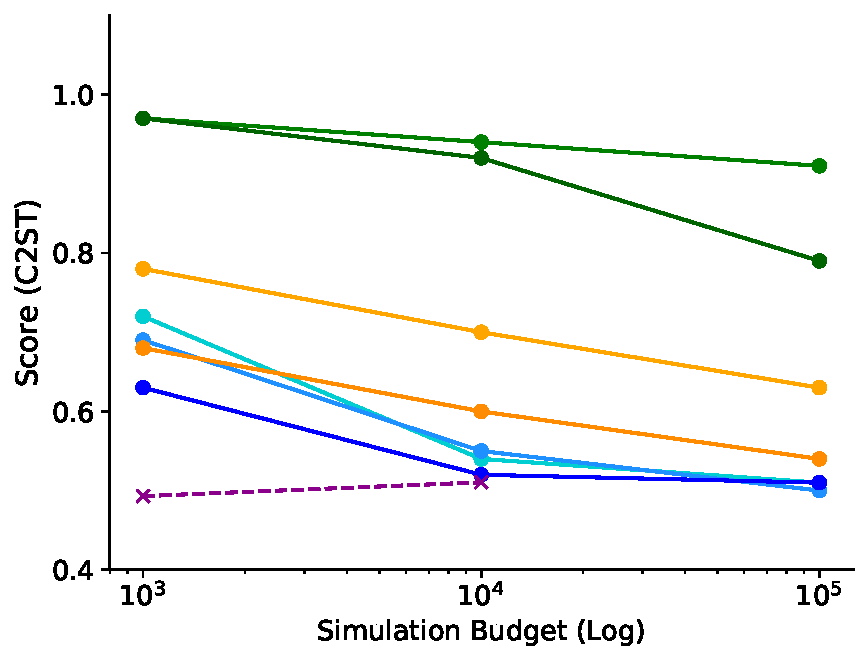
\includegraphics[width=.4\linewidth]{./figures/gaussian_linear_uniform.pdf}
%   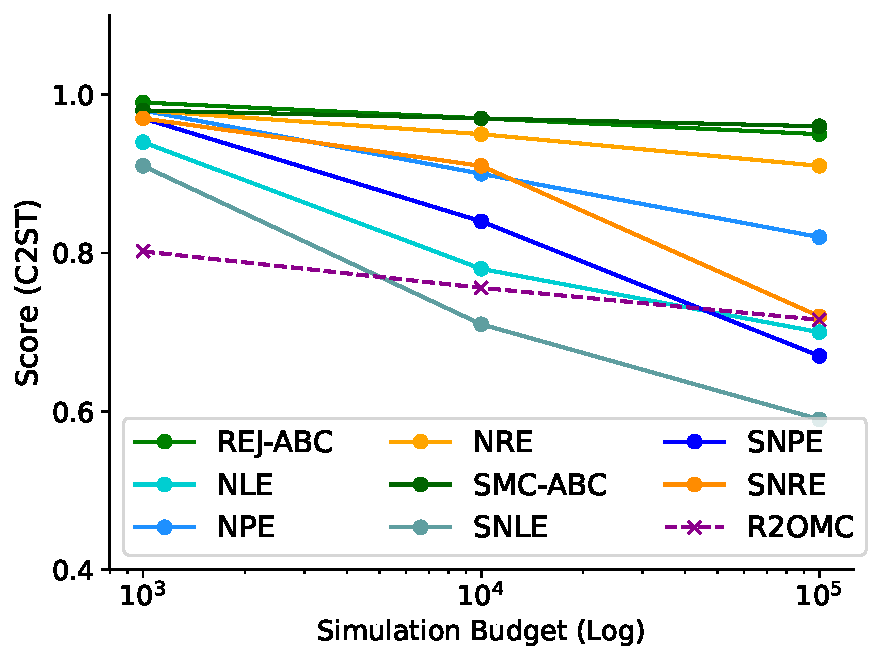
\includegraphics[width=.4\linewidth]{./figures/slcp.pdf}
%   \caption{Left---T.2: Gaussian Linear Uniform. Right---T.3: SLCP.}
%   \label{fig:exp_sbi_extra}
% \end{figure}

\subsection{MoG - Shifted Gaussian}

This additional experiment uses a simulator that samples from a mixture of two Gaussians, whose means are shifted by a constant value.

\begin{tabular}{@{}ll@{}}
  \textbf{Prior} & $\thb \sim \mathcal{U}(-15, 15)^4$ \\[5pt]
  \textbf{Simulator} & $\yb \sim \frac{1}{2} \left ( \mathcal{N}(\thb + \mathbf{5}, \mathbf{I}) + \mathcal{N}(\thb, \mathbf{I}) \right )$ \\[5pt]
  \textbf{Dimensionality} & $\thb \in \mathbb{R}^{4}$, $\yb \in \mathbb{R}^{4}$ \\[5pt]
\end{tabular}

We will use two separate cases: one with $N=4$ similar observations and another with $N=4$ different observations.
In both cases, the posterior is:
%
\begin{align}
  \label{eq:gauss_mult_obs}
  p(\thb|\{\data_n\}) &\propto p(\thb) p(\{\data_n\}|\thb) \\
                      &\propto p(\thb) \prod_{n=1}^{N} p(\data_n|\thb) \label{eq:gauss_mult_obs_1} \\
                      &\propto \mathcal{U}(-\mathbf{15},\mathbf{15}) \prod_{n=1}^{N} \dfrac{1}{2} \left ( \mathcal{N}(\data_n; \thb + \mathbf{5}, \mathbf{I}) + \mathcal{N}(\data_n; \thb, \mathbf{I}) \right ) \\
                      &\propto \mathcal{U}(-\mathbf{15},\mathbf{15}) \prod_{n=1}^{N} \dfrac{1}{2}\left ( \mathcal{N}(\thb; \data_n - \mathbf{5}, \mathbf{I}) + \mathcal{N}( \thb; \data_n, \mathbf{I}) \right ) \label{eq:gauss_mult_obs_3}\\
                      &\appropto \prod_{n=1}^{N} \left ( \mathcal{N}(\thb; \data_n - \mathbf{5}, \mathbf{I}) + \mathcal{N}( \thb; \data_n, \mathbf{I}) \right ) \label{eq:gauss_mult_obs_4}
\end{align}
In~(\ref{eq:gauss_mult_obs_1}), the factorization is due to the $N$ independently and identically distributed (iid) data points.
In~(\ref{eq:gauss_mult_obs_3}), we apply the property: $\mathcal{N}(\yb; \thb + \mub, \Sigma) = \mathcal{N}(\thb; \yb - \mub, \Sigma)$.
In~(\ref{eq:gauss_mult_obs_4}), we use that the data that we will use are sufficiently far from the boundaries so that we may ignore the boundary effects in the truncated distribution.

\paragraph{Case 1:}

In Case 1, we use $N=4$ similar observations: $\data_n \approx (0, \ldots, 0)$ for $n \in \{ 1, \ldots, N \}$. The ground-truth posterior is approximately:
%
\begin{equation}
  p(\thb | \data) \approx \mathcal{N}(\thb; - \mathbf{5}, \frac{1}{N} \mathbf{I}) + \mathcal{N}(\thb; \mathbf{0}, \frac{1}{N} \mathbf{I})
  \label{eq:mog_shifted_gaussian_case_1}
\end{equation}
%
\textbf{Proof.}
%
\begin{align} 
p(\thb|{\data_n}) 
&\appropto \prod_n^{N} \left ( \mathcal{N}(\thb; \data_n - \mathbf{5}, \mathbf{I}) + \mathcal{N}( \thb; \data_n, \mathbf{I}) \right ) \\
&\appropto \left( \mathcal{N}(\thb; - \mathbf{5}, \mathbf{I}) + \mathcal{N}(\thb; \mathbf{0}, \mathbf{I}) \right)^N \\
&\appropto \sum_{n=0}^N \binom{N}{n} (\mathcal{N}(\thb; - \mathbf{5}, \mathbf{I}))^n (\mathcal{N}(\thb; \mathbf{0}, \mathbf{I}))^{N-n} \\
&\appropto \left( \mathcal{N}(\thb; - \mathbf{5}, \mathbf{I}) \right)^N + \left( \mathcal{N}( \thb; \mathbf{0}, \mathbf{I}) \right)^N \label{eq:gauss_mult_obs_case_1_1}  \\
&\appropto \mathcal{N}(\thb; - \mathbf{5}, \frac{1}{N}\mathbf{I}) + \mathcal{N}( \thb; \mathbf{0}, \frac{1}{N}\mathbf{I}) \label{eq:gauss_mult_obs_case_1_2} 
\end{align}
%
In (\ref{eq:gauss_mult_obs_case_1_1}), for $n \in \{1, \ldots, N-1\}$ the terms involve products between 
$\mathcal{N}(\thb; - \mathbf{5}, \mathbf{I})$ and $ \mathcal{N}( \thb; \mathbf{0}, \mathbf{I})$ so they have 
a much smaller magnitude compared to $(\mathcal{N}(\thb; - \mathbf{5}, \mathbf{I}))^N$ ($n=N$) and $\mathcal{N}(( \thb; \mathbf{0}, \mathbf{I}))^N$ ($n=0$).
This allows us to approximate the expression by retaining only these two dominant terms.
In (\ref{eq:gauss_mult_obs_case_1_2}), we use the property that raising a Gaussian distribution to the power \(N\) results in a Gaussian with the same mean and a covariance scaled by \(\frac{1}{N}\). 
% In Figure~\ref{fig:multi_obs_case_1_gt} we show two dimensions, $\thb_i$ and $\thb_j$, of the ground truth posterior for $N=\{1, 4, 10, 20\}$ observations.

\paragraph{Case 2:}

In Case 2, we use an even number of $N$ observations that are split in two categories, 
half around $(0, \ldots, 0)$, i.e., 
$\data_n \approx (0, \ldots, 0)$ for $n \in \{ 1, \ldots, N/2 \}$ and the other half around 
$(5, \ldots, 5)$, i.e., 
$\data_n \approx (5, \ldots, 5)$ for $n \in \{ N/2 + 1, \ldots, N \}$.
The posterior, for values of $\thb$ sufficienty far from the boundary, is:
\begin{equation}
  p(\thb | \data) \approx \mathcal{N}(\thb; \mathbf{0}, \frac{1}{N} \mathbf{I})
  \label{eq:mog_shifted_gaussian_case_2}
\end{equation}

\textbf{Proof.}
\begin{align}
  p(\thb|\{\data_k\}) 
  &\appropto \prod_n^{N} \left ( \mathcal{N}(\thb; \data_n - \mathbf{5}, \mathbf{I}) + \mathcal{N}( \thb; \data_n, \mathbf{I}) \right ) \\
  &\appropto \prod_{n=1}^{N/2} \left ( \mathcal{N}(\thb; - \mathbf{5}, \mathbf{I}) + \mathcal{N}( \thb; \mathbf{0}, \mathbf{I}) \right ) \prod_{n=N/2 + 1}^{N} \left ( \mathcal{N}(\thb; \mathbf{0}, \mathbf{I}) + \mathcal{N}( \thb; \mathbf{5}, \mathbf{I}) \right )  \\
  &\appropto \prod_{n=1}^{N/2} \left ( \mathcal{N}(\thb; - \mathbf{5}, \mathbf{I}) + \mathcal{N}( \thb; \mathbf{0}, \mathbf{I}) \right ) \prod_{n=1}^{N/2} \left ( \mathcal{N}(\thb; \mathbf{0}, \mathbf{I}) + \mathcal{N}( \thb; \mathbf{5}, \mathbf{I}) \right )  \\
  &\appropto \left ( ( \mathcal{N}(\thb; - \mathbf{5}, \mathbf{I}) )^{N/2} + ( \mathcal{N}( \thb; \mathbf{0}, \mathbf{I}) )^{N/2} \right ) \left ( ( \mathcal{N}(\thb; \mathbf{0}, \mathbf{I}) )^{N/2} + ( \mathcal{N}( \thb; \mathbf{5}, \mathbf{I}) )^{N/2} \right ) \label{eq:gauss_mult_obs_case_2_1} \\
  &\appropto \mathcal{N}(\thb; \mathbf{0}, \mathbf{I})^N \label{eq:gauss_mult_obs_case_2_2} \\
  &\appropto \mathcal{N}( \thb; \mathbf{0}, \frac{1}{N}\mathbf{I}) \label{eq:gauss_mult_obs_case_2_3}
\end{align}
%
In (\ref{eq:gauss_mult_obs_case_2_1}), we keep only the dominant terms, as in Case 1.
In (\ref{eq:gauss_mult_obs_case_2_2}), we use that terms that involve combinations of \(\mathcal{N}(\thb; \mathbf{0}, \mathbf{I})^{N/2}\), \(\mathcal{N}(\thb; -\mathbf{5}, \mathbf{I})^{N/2}\) and \(\mathcal{N}(\thb; \mathbf{5}, \mathbf{I})^{N/2}\) have significantly smaller magnitudes compared to the dominant ones; \(\mathcal{N}(\thb; \mathbf{0}, \mathbf{I})^{N/2} \mathcal{N}(\thb; \mathbf{0}, \mathbf{I})^{N/2}\).
In (\ref{eq:gauss_mult_obs_case_2_3}), we use the property that raising a Gaussian distribution to the power \(N\) results in a Gaussian with the same mean and a covariance scaled by \(\frac{1}{N}\).
% In Figure~\ref{fig:multi_obs_case_2_gt} we show two dimensions, $\thb_i$ and $\thb_j$, of the ground truth posterior for $N=\{1, 4, 10, 20\}$ observations.

\paragraph{Results.}

Figure~\ref{fig:multi_obs} demonstrates that \rromc~aligns closely with the ground truth posterior, correctly capturing the two modes in Case 1 and the single mode in Case 2.
% Due to the approximation error introduced by $\epsilon$, \rromc~exhibits a slightly higher variance compared to the ground truth.
In contrast, both \romc~struggles with multiple observations, resulting in their samples being distributed along the \(45^{\circ}\) line.

\begin{figure}
    \centering
    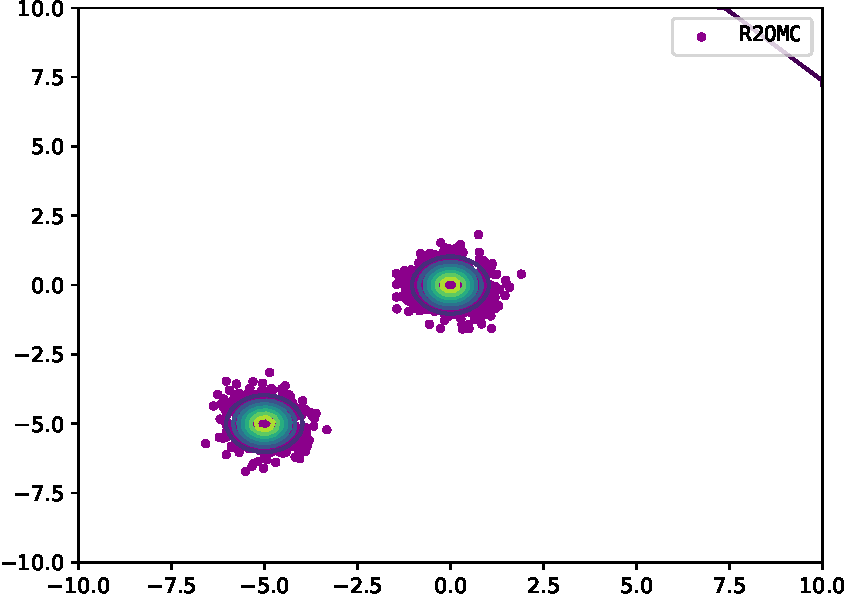
\includegraphics[width=0.23\linewidth]{figures/old/multi_obs_case_1_iterative_romc}
    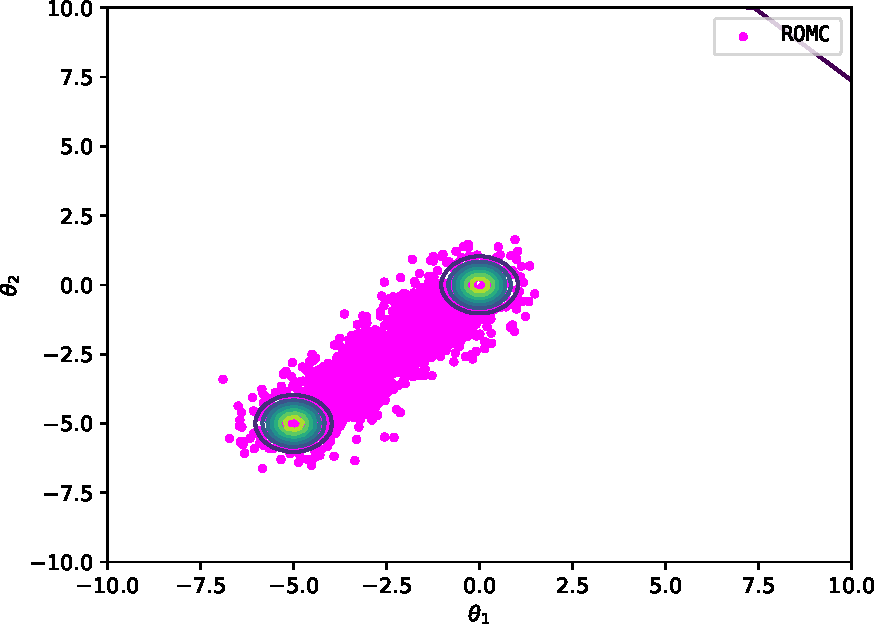
\includegraphics[width=0.23\linewidth]{figures/old/multi_obs_case_1_romc}
    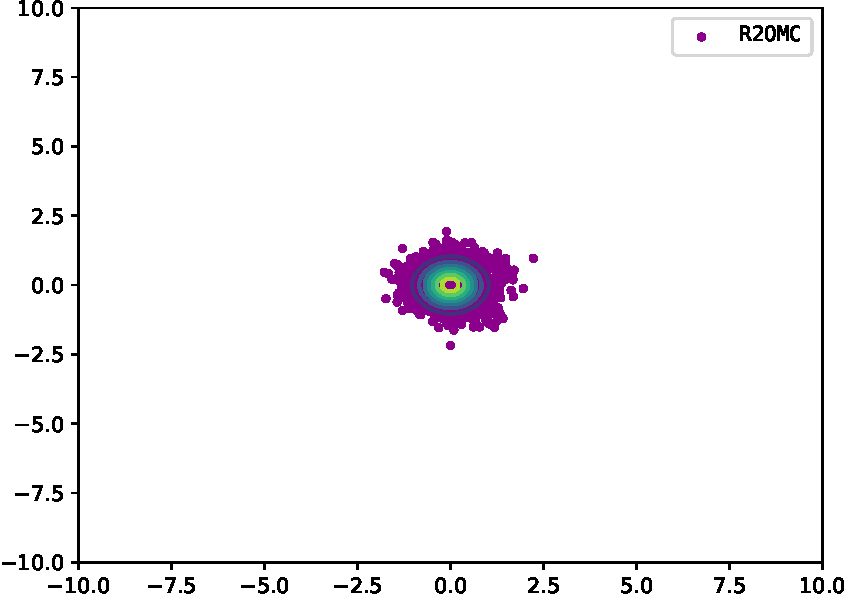
\includegraphics[width=0.23\linewidth]{figures/old/multi_obs_case_2_iterative_romc}
    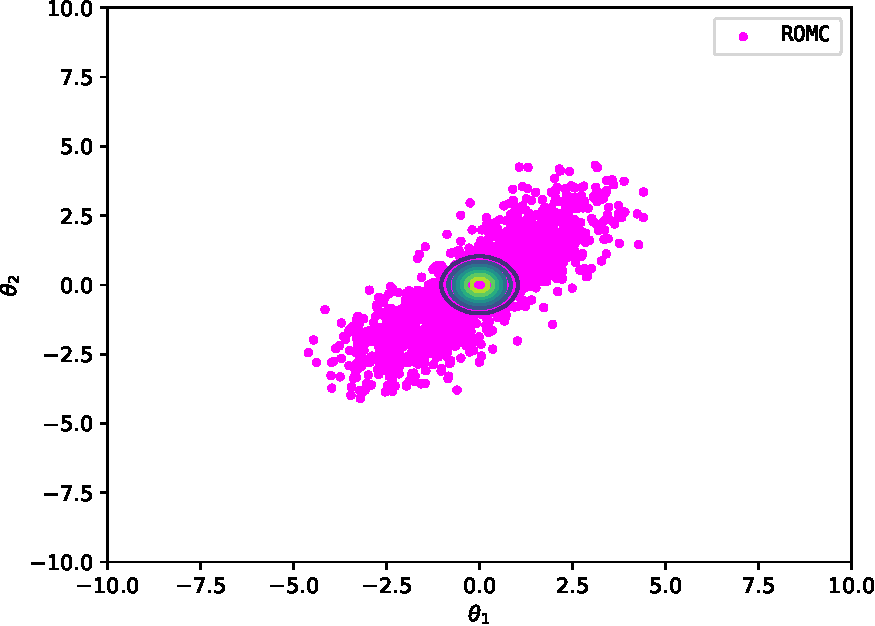
\includegraphics[width=0.23\linewidth]{figures/old/multi_obs_case_2_romc}
    \caption{From left to right: R2OMC on Case 1, Naive-ROMC on Case 1, R2OMC on Case 2, and Naive-ROMC on Case 2.}
    \label{fig:multi_obs}
\end{figure}


\end{document}
